% Options for packages loaded elsewhere
\PassOptionsToPackage{unicode}{hyperref}
\PassOptionsToPackage{hyphens}{url}
%
\documentclass[
  letterpaper,
]{book}

\usepackage{amsmath,amssymb}
\usepackage{iftex}
\ifPDFTeX
  \usepackage[T1]{fontenc}
  \usepackage[utf8]{inputenc}
  \usepackage{textcomp} % provide euro and other symbols
\else % if luatex or xetex
  \usepackage{unicode-math}
  \defaultfontfeatures{Scale=MatchLowercase}
  \defaultfontfeatures[\rmfamily]{Ligatures=TeX,Scale=1}
\fi
\usepackage{lmodern}
\ifPDFTeX\else  
    % xetex/luatex font selection
\fi
% Use upquote if available, for straight quotes in verbatim environments
\IfFileExists{upquote.sty}{\usepackage{upquote}}{}
\IfFileExists{microtype.sty}{% use microtype if available
  \usepackage[]{microtype}
  \UseMicrotypeSet[protrusion]{basicmath} % disable protrusion for tt fonts
}{}
\makeatletter
\@ifundefined{KOMAClassName}{% if non-KOMA class
  \IfFileExists{parskip.sty}{%
    \usepackage{parskip}
  }{% else
    \setlength{\parindent}{0pt}
    \setlength{\parskip}{6pt plus 2pt minus 1pt}}
}{% if KOMA class
  \KOMAoptions{parskip=half}}
\makeatother
\usepackage{xcolor}
\setlength{\emergencystretch}{3em} % prevent overfull lines
\setcounter{secnumdepth}{5}
% Make \paragraph and \subparagraph free-standing
\makeatletter
\ifx\paragraph\undefined\else
  \let\oldparagraph\paragraph
  \renewcommand{\paragraph}{
    \@ifstar
      \xxxParagraphStar
      \xxxParagraphNoStar
  }
  \newcommand{\xxxParagraphStar}[1]{\oldparagraph*{#1}\mbox{}}
  \newcommand{\xxxParagraphNoStar}[1]{\oldparagraph{#1}\mbox{}}
\fi
\ifx\subparagraph\undefined\else
  \let\oldsubparagraph\subparagraph
  \renewcommand{\subparagraph}{
    \@ifstar
      \xxxSubParagraphStar
      \xxxSubParagraphNoStar
  }
  \newcommand{\xxxSubParagraphStar}[1]{\oldsubparagraph*{#1}\mbox{}}
  \newcommand{\xxxSubParagraphNoStar}[1]{\oldsubparagraph{#1}\mbox{}}
\fi
\makeatother


\providecommand{\tightlist}{%
  \setlength{\itemsep}{0pt}\setlength{\parskip}{0pt}}\usepackage{longtable,booktabs,array}
\usepackage{calc} % for calculating minipage widths
% Correct order of tables after \paragraph or \subparagraph
\usepackage{etoolbox}
\makeatletter
\patchcmd\longtable{\par}{\if@noskipsec\mbox{}\fi\par}{}{}
\makeatother
% Allow footnotes in longtable head/foot
\IfFileExists{footnotehyper.sty}{\usepackage{footnotehyper}}{\usepackage{footnote}}
\makesavenoteenv{longtable}
\usepackage{graphicx}
\makeatletter
\def\maxwidth{\ifdim\Gin@nat@width>\linewidth\linewidth\else\Gin@nat@width\fi}
\def\maxheight{\ifdim\Gin@nat@height>\textheight\textheight\else\Gin@nat@height\fi}
\makeatother
% Scale images if necessary, so that they will not overflow the page
% margins by default, and it is still possible to overwrite the defaults
% using explicit options in \includegraphics[width, height, ...]{}
\setkeys{Gin}{width=\maxwidth,height=\maxheight,keepaspectratio}
% Set default figure placement to htbp
\makeatletter
\def\fps@figure{htbp}
\makeatother

\makeatletter
\@ifpackageloaded{bookmark}{}{\usepackage{bookmark}}
\makeatother
\makeatletter
\@ifpackageloaded{caption}{}{\usepackage{caption}}
\AtBeginDocument{%
\ifdefined\contentsname
  \renewcommand*\contentsname{Table of contents}
\else
  \newcommand\contentsname{Table of contents}
\fi
\ifdefined\listfigurename
  \renewcommand*\listfigurename{List of Figures}
\else
  \newcommand\listfigurename{List of Figures}
\fi
\ifdefined\listtablename
  \renewcommand*\listtablename{List of Tables}
\else
  \newcommand\listtablename{List of Tables}
\fi
\ifdefined\figurename
  \renewcommand*\figurename{Figure}
\else
  \newcommand\figurename{Figure}
\fi
\ifdefined\tablename
  \renewcommand*\tablename{Table}
\else
  \newcommand\tablename{Table}
\fi
}
\@ifpackageloaded{float}{}{\usepackage{float}}
\floatstyle{ruled}
\@ifundefined{c@chapter}{\newfloat{codelisting}{h}{lop}}{\newfloat{codelisting}{h}{lop}[chapter]}
\floatname{codelisting}{Listing}
\newcommand*\listoflistings{\listof{codelisting}{List of Listings}}
\makeatother
\makeatletter
\makeatother
\makeatletter
\@ifpackageloaded{caption}{}{\usepackage{caption}}
\@ifpackageloaded{subcaption}{}{\usepackage{subcaption}}
\makeatother

\ifLuaTeX
  \usepackage{selnolig}  % disable illegal ligatures
\fi
\usepackage{bookmark}

\IfFileExists{xurl.sty}{\usepackage{xurl}}{} % add URL line breaks if available
\urlstyle{same} % disable monospaced font for URLs
\hypersetup{
  pdftitle={Weikersheim, Residenzschloss},
  pdfauthor={Team Redaktion},
  hidelinks,
  pdfcreator={LaTeX via pandoc}}


\title{Weikersheim, Residenzschloss}
\author{Team Redaktion}
\date{2024-03-22}

\begin{document}
\frontmatter
\maketitle

\renewcommand*\contentsname{Table of contents}
{
\setcounter{tocdepth}{2}
\tableofcontents
}

\mainmatter
\bookmarksetup{startatroot}

\chapter{Katalog zur Ausstellung: Der Große Saal
(Rittersaal)}\label{katalog-zur-ausstellung-der-grouxdfe-saal-rittersaal}

Ein Katalog mit Kunstwerken aus der CbDD-Sammlung. Textteil:
\href{https://www.deckenmalerei.eu/42d06165-58e7-4653-bfe4-3d5f7091fc33\#6e73f774-4b7f-4e37-937b-e11cc35c5bc8}{6e73f774-4b7f-4e37-937b-e11cc35c5bc8}

Großer Saal (Rittersaal) {[}Raum{]} Name: Großer Saal (Rittersaal) ID:
15685f4a-3727-4110-8967-1d8287431997 Typ: Raum Länge (m): 36.4 Breite
(m): 11.7 Höhe (m): 8.25 Funktion {[}Raum{]}: Saal -\textgreater{}
Hauptsaal Datierung {[}Raum{]}: 1601-1605 hat Auftraggeber: Wolfgang
II., Hohenlohe-Weikersheim, Graf {[}Person{]} hat Auftraggeber: Carl
Ludwig, Hohenlohe-Weikersheim, Graf {[}Person{]} hat Teil: Malerei des
Barock {[}Malerei{]} hat Teil: Malerei der Renaissance {[}Malerei{]} hat
Stuckateur: Schmidt, Gerhard {[}Person{]} hat Stuckateur: Limmerich,
Christoph {[}Person{]} hat Bildhauer: Juncker, Michael {[}Person{]} ist
dokumentiert in: Der Große Saal (Rittersaal) {[}Textteil{]} ist Teil
von: Erschließungsraumfolgen {[}Raumfolge{]} Erstellung des Datensatzes:
2020-05-19, 11:18 letzte Bearbeitung: 2023-10-16, 14:28

This work is licensed under a Creative Commons
Attribution-NonCommercial-NoDerivs 4.0 International License.

\bookmarksetup{startatroot}

\chapter{Impressum}\label{impressum}

Veröffentlichungsmetadaten, die aus dem Thoth.pub GraphQL API.
\url{https://api.thoth.pub/graphiql}

Katalog zur Ausstellung: Der Große Saal (Rittersaal) Weikersheim,
Residenzschloss

Open Science Lab - TIB Hannover

First published 2024-04-16

Copyright © The authors 2024 Licensed as
https://creativecommons.org/licenses/by-nc-nd/4.0/

DOI: https://doi.org/10.5281/zenodo.10977822

\bookmarksetup{startatroot}

\chapter{Essay}\label{essay}

Get data of text items from wikibase

Wikibase link:
\url{https://computational-publishing-service.wikibase.cloud/entity/Q209}

Kurator: Seeger, Ulrike

\bookmarksetup{startatroot}

\chapter{Bau-, Ausstattungs- und
Funktionsgeschichte}\label{bau--ausstattungs--und-funktionsgeschichte}

Die hervorragend erhaltene wandfeste Ausstattung des Großen Saals, der
1639 als „großer Saahl`` {[}1{]} geführt wurde und seinen heute
geläufigen Namen Rittersaal erst im Nachhinein erhielt, datiert aus den
Jahren 1601 bis 1605. Am Beginn stand den Quellen zufolge der
monumentale Saalkamin. Der Vertrag mit dem Bildhauer Michael Juncker aus
Miltenberg datiert vom 7. September 1601.{[}2{]} Im November 1601 wurden
mit Balthasar Katzenberger die Deckengemälde verdingt, der die Arbeiten
13 Monate später Anno 1602 abschloss.{[}3{]} 1603 signierte und datierte
der Kalkschneider Gerhard Schmidt das Portal an der inneren
Ostseite.{[}4{]} Die Jahreszahl 1605 zusammen mit den Initialen CL für
den Kalkschneider Christoph Limmerich über der Tür zum Altan markieren
den Abschluss der Arbeiten.{[}5{]}

Seit 1710/11 wurde der Saal unter Graf Carl Ludwig behutsam dem barocken
Zeitgeschmack angepasst und inhaltlich vom Jagd- zum gräflichen
Rittersaal umgedeutet. Christian Thalwitzer hatte Balthasar
Katzenbergers Deckengemälde „im großen Saal {[}zu{]} übermahlen, genau
durch{[}zu{]}gehen und wo es Schaden genommen, mit allem Fleyß``
auszubessern.{[}6{]} Bei dieser Gelegenheit versah er die Gemälderahmen
und die dazwischenliegenden Stuckrippen mit der bis heute gültigen roten
Marmorierung.{[}7{]} An den Wänden wurden die Roll- und
Beschlagwerkkartuschen der Schmuckzone ebenfalls rot marmoriert und an
Kamin und Innenportal die rot marmorierten Schattenrahmen hinzugefügt.

In einem zweiten Schritt wurde der Sockel ringsum mit rot marmorierten
Lambris versehen, die Christian Thalwitzer im Rechnungsjahr 1715/16 mit
51 Schloss- und Gartenveduten im Querformat{[}8{]} und 27 Orangenbäumen
und anderen exotischen Kübelpflanzen im Hochformat bemalte. Die 12
ganzfigurigen Porträts männlicher Vorfahren zum Teil in Ritterrüstung,
die dem Rittersaal seinen heutigen Namen gaben, schuf bereits 1710 Peter
Franz Tassaert aus Rothenburg.{[}9{]}

\section{\texorpdfstring{\textbf{Beschreibung des
Raumes}}{Beschreibung des Raumes}}\label{beschreibung-des-raumes}

Der 36,4 Meter lange, 11,7 Meter breite und 8,25 Meter hohe Saal{[}10{]}
wird durch hohe segmentbogenförmige Fensternischen gegliedert, deren
Achsen von großen Okuli weitergeführt werden. Im Gegenzug zu dieser
Vertikalen beschränkt sich der reiche Stuckdekor friesartig auf die
obere Wandzone, die oberhalb eines Gesimses auf der Höhe des oberen
Drittels der Fenster beginnt. Dadurch, dass sich die Stuckdekoration in
das obere Drittel der Fensterlaibungen hineinzieht, erwecken sie den
Eindruck hoheitsvoll gestelzter Bögen.{[}11{]}

An der Westwand, neben der im ersten Joch der Hofseite der Saal über die
Wendeltreppe betreten wird, erhebt sich ein monumentaler Kamin. Mit
Kaminöffnung, Attikafeld und rundbogigem Auszug umfasst er drei Zonen,
von denen Attika und Auszug in der Höhe der stuckierten Wandzone des
Saals entsprechen. An der Ostwand, wo man den Saal Richtung Tafelstube
verlässt, befindet sich ein prächtiges, 1603 datiertes stuckiertes
Innenportal des Kalkschneiders Gerhard Schmidt.{[}12{]} Darüber
verläuft, teilweise hinter dem Attikarelief, eine Empore beispielsweise
für Musiker.

Den Kamin flankieren stuckierte Darstellungen des Grafenpaars Wolfgang
II. von Hohenlohe und Magdalena, geborene Prinzessin von
Nassau-Katzenelnbogen mit ihrer jeweiligen Ahnenprobe.{[}13{]} Dem Graf
wurde die zeremoniell höherrangige Seite heraldisch rechts des Kamins,
der Gräfin die Seite heraldisch links des Kamins zugeteilt. Graf und
Gräfin liegen jeweils auf der Seite einander abgewandt und blicken mit
aufgestütztem Kopf in den Saal. Aus ihnen heraus wächst in der Art einer
Wurzel Jesse die über fünf Generationen geführte Ahnenprobe. Der Graf
trägt eine Rüstung mit Waffenrock und stützt seinen Ellenbogen auf einen
Helm. Die Gräfin hat zwei Kinder im Arm, von denen das vordere ein Junge
ist.

An den beiden Längsseiten nimmt die stuckierte Schmuckzone weit
vorkragende, gleichfalls stuckierte Wandskulpturen wilder Tiere auf. Sie
beziehen sich einerseits auf das Programm der Decke, das der höfischen
Jagd in all ihren Ausformungen gewidmet ist. Andererseits sind sie auf
die Kaminwand ausgerichtet, die mit ihren nachstehend zu erläuternden
Bildthemen als Stellvertreter des Grafen, seiner konfessionellen
Einstellung und seiner dynastischen Herkunft konzipiert ist. Zusammen
mit einer gemalten Darstellung des lyraspielenden Orpheus an der Decke
erlauben die Tiere in ihrer Ausrichtung auf den Kamin die Identifikation
des Grafen mit Orpheus als Sinnbild des guten Herrschers. Diese hier
erstmals entwickelte Deutung wird unten im Abschnitt „Programm und
Synthese der Saalausstattung der Renaissance`` vorgetagen.

\section{Kamin und Innenportal}\label{kamin-und-innenportal}

Der Kamin aus Andernacher Tuffstein von Michael Juncker und seinen
Söhnen Hans und Zacharias aus Miltenberg präsentiert im Hauptrelief als
zentrales Motiv die persönliche Devise des Grafen Wolfgang. Die
Entschlüsselung der im Vertrag vom September 1601 vereinbarten „ihrer
gnaden Diviso``{[}14{]} gelang erst vor wenigen Jahren Jürgen
Kniep.{[}15{]} Dargestellt ist ein antikisch gekleideter Krieger,
umgeben von den Symbolen der Kardinal- und theologischen Tugenden. Die
Devise „Gott gibt Glück`` lässt den reformatorischen Glauben des Grafen
Wolfgang ebenso erkennen wie die Betonung der Liebe (Herz in der linken
Hand des Kriegers) und des Buches, aus dem die Schlange ihre Weisheit
bezieht. Im Sinne der protestantischen Rechtfertigungslehre oblag es
nicht dem Klerus, sondern allein Gott, dem Menschen Gnade angedeihen zu
lassen.

Als räumliches Gegenstück zum skulptierten Kamin entstand 1603 in einem
Paragone der Techniken und Materialien das monumentale, aus Stuck
gefertigte Innenportal an der Ostseite. Sein Aufbau ist wie der Kamin
dreizonig mit rundbogiger Öffnung, Attikarelief und Auszug. Der
Kalkschneider Gerhard Schmidt, der das Portal selbstbewusst mit seinen
Initialen signiert hat, hat in der Türkenschlacht des Hauptreliefs mit
extrem hinterschnittenen Pferde- und Soldatenleibern den moderater
skulptierten Steinkamin an Kunstfertigkeit übertroffen. Einen Höhepunkt
der Stuckateurskunst der Zeit bildet der vollplastisch gearbeitete
heilige Georg auf seinem zum Sprung über den Drachen ansetzenden Pferd.

Das Portal ist inhaltlich auf den ältesten Sohn des Grafen Wolfgang,
Georg Friedrich, zu beziehen, der im Rang eines Obristen des Fränkischen
Reichskreises und auch der kaiserlichen Armee im Langen Türkenkrieg
(1593--1606) kämpfte.{[}16{]} Als einer seiner größten Erfolge gilt die
versuchte Einnahme der Festung Gran (Eszergom) im Jahr 1594, an der er
als kaiserlicher Obrist beteiligt war.{[}17{]} Die Festung, vor der sich
auf dem Relief das Schlachtengetümmel abspielt, stellt in der Tat
Eszergom da, was an der Höhenlage und der Zweiturmfassade der Kathedrale
zu erkennen ist.{[}18{]} Der das Portal bekrönende heilige Georg als
Drachentöter mit Lanze und zugleich Namenspatron des Erbprinzen sowie
Patron der Stadtkirche wäre im Sinne des Protestantismus als
tugendhafter Bezwinger des Bösen zu deuten.{[}19{]} Mit der Thematik des
Langen Türkenkriegs bereitete das Portal auf die dahinterliegende
Tafelstube vor, für deren Decke Balthasar Katzenberger 12 große
Belagerungsszenen auf Leinwand malte.

Das Portal von 1603 war aber nicht nur heroisch gestimmt. In den
Zwickeln lagern Putti, die als Mahnung an die Endlichkeit des Lebens dem
Betrachter ein Stundenglas, eine Sense und einen Schlüssel -- vielleicht
ins Himmelreich -- vor Augen halten.

\section{Das Mobiliar}\label{das-mobiliar}

Die renaissancezeitliche Ausstattung des Saals mit Mobilien geht aus
einem 1625--1627 aufgenommenen Inventar hervor.{[}20{]} Die als erstes
genannten „Ein und zwanzig Stuck goldt uf Leder tappezerey`` dürften als
goldgeprägte Ledertapeten die Trumeaus zwischen den Fenstern geziert
haben. Ledertapeten waren kostbar, was sich in ihrer erstplatzierten
Nennung niederschlug.{[}21{]} An Stellmöbeln beinhaltete der Saal „Zwo
lange Tafel`` und „Ein und dreissig von goldt uff Lederne Sessel``. Die
Wände schmückten zusätzlich zu den Ledertapeten „Sechzehn gemahlte
Tafeln``, also im Sujet nicht näher charakterisierte Gemälde. Die
Beleuchtung erfolgte über „Acht große hülzerne Lichter, gemahlt``.

Vier Gemälde wurden zusätzlich zu den sechzehn aufgeführt, da sie
vermutlich im Vorgängerinventar des Grafen Wolfgang, das dem Inventar
als Vorlage diente, noch nicht enthalten waren. Sie stellten „Kaiser
Matthie und der Kayserin / Item Meines Gnd. Herrn und gnl. Frawen
Abcontrafehung`` dar. Kaiser Matthias regierte in den Jahren 1612--1619,
seine Gemahlin Anna von Österreich-Tirol starb 1618. Die Gemälde
stammten demnach aus der Zeit des Grafen Georg Friedrich von
Hohenlohe-Weikersheim, der mit Eva von Waldstein verheiratet war.

{[}1{]} HZAN La 130 Bü 152, Schadensinventar von 1639. Die Kenntnis und
die Transkription dieser Archivalie verdankt die Autorin Frieder
Leipold.

{[}2{]} Der erhaltene Vertrag (HZAN We 50 D6) in Transkription bei
Freeden, Kamin, 1950, S. 144--145. Bezahlt wurde Juncker im Oktober
1602.

{[}3{]} Poser, Deckenbilder, 1980, S. 160--161.

{[}4{]} Merten, Weikersheim, o. J., S. 44. Drös, Inschriften
Mergentheim, 2002, S. 244. Zum Oeuvre und Lebensweg des Kalkschneiders
Gerhard Schmidt: Kreder, Hellenstein, 2005/2006; Rinn-Kupka, Stuck,
2018, S. 126--129; Lange, ‚welsche Kamin`, 2019.

{[}5{]} Merten, Weikersheim, o. J., S. 44. Drös, Inschriften
Mergentheim, 2002, S. 254.

{[}6{]} Fandrey, Weikersheim, 2010, S. 55.

{[}7{]} Dieser Befund kam bei der Restaurierung der Jahre 1995--1997
zutage. Für zahlreiche Informationen und die Übermittlung des
Abschlussberichts vom 05.03.1998 dankt die Autorin Herrn Dipl.-Ing. Erik
Reinhold, Staatliches Hochbauamt Heilbronn.

{[}8{]} Die Vedute des Carlsberg bei Weikersheim kam erst 1747 im
Zusammenhang mit der damals aufgestellten Kunstuhr hinzu, doch dürfte
sie eine ältere Vedute am Fensterpfeiler hinter der Uhr ersetzt haben.

{[}9{]} Valentin, Malerische Lebensläufe, 2019, Anm. 11. Zu Tassaert
liegt ein Lebenslauf mit Werkverzeichnis vor: Schnurrer, Tassaert, 2014.

{[}10{]} Die genauen Maße gibt Walther-Gerd Fleck (Weyer, Georg Stegle,
2017, S. 52).

{[}11{]} Vgl. dagegen Gebeßler, Saal Süddeutschland, 1957, S. 49, der
die Fensternischen aufgrund ihrer Dekoration als Anräume empfindet.

{[}12{]} Das Portal wird in der Literatur zu Unrecht als Eingangsportal
in den Saal beschrieben (Poser, Deckenbilder, 1980, S. 160; Kniep,
Glück, 2005, S. 52 und 59; Käpplinger, Jagd, 2011, S. 73). Es ist jedoch
nach innen gerichtet, führt also von innen nach außen. Außerdem folgt in
der Wegeführung eines Renaissanceschlosses die Tafelstube auf den
Rittersaal. Auch der Betrachterstandpunkt der Deckengemälde ist mit dem
Rücken zum Kamin so ausgerichtet, dass man die Bilder vom Kamin kommend,
Richtung Tafelstube gehend bewundert.

{[}13{]} Zu den Ahnenproben: Drös, Inschriften Mergentheim, 2002, S.
255--261. Außerdem Kniep, Glück, 2005, S. 48--52.

{[}14{]} Freeden, Kamin, 1950, S. 144.

{[}15{]} Kniep, Glück, 2005, S. 57--74. Weiterführende Gedanken und
Literatur zur Bildhauerfamilie Juncker liefert: Lange, ‚welsche Kamin`,
2019.

{[}16{]} Kniep, Glück, 2005, S. 52--57. Außerdem Findbuch HZAN La 130 Bü
102 (Bestallung zum Obristen des Fränkischen Reichskreises, 1598) und La
130 Bü 108 (Teilnahme als kaiserlicher Obrist am Feldzug gegen die
Türken 1603).

{[}17{]} Trentin-Meyer, Georg Friedrich von Hohenlohe, 2019, S. 90. Vgl.
Niederkorn, Langer Türkenkrieg, 1993, S. 11.

{[}18{]} Außerdem als Beleg die Darstellung in: Ortelius, Chronologia,
1602, Tf. „Wahre Contrafactur der Belagerung Gran, sampt der Schlacht so
dabei geschehen, den 3. Augusti. Anno 1595``. Ortelius wählte für seine
Illustration die erfolgreiche Belagerung und Schlacht von 1595. Die
Belagerung von 1594 war für die Kaiserlichen noch nicht erfolgreich.

{[}19{]} Kniep, Glück, 2005, S. 56.

{[}20{]} Auszüge des Inventars stellte freundlicherweise Dinah
Rottschäfer der Autorin zur Verfügung.

{[}21{]} Bei dem von Käpplinger, Auf's Schönste, 2019, S. 189 mit Anm. 3
genannten Inventar von 1634 handelt es sich um einen Schadensbericht, in
dem die Ledertapeten verkürzt als „tappezereien von gold`` bezeichnet
wurden, was Käpplinger in Unkenntnis des Vorgängerinventars als textile
Wandbespannungen deutete.

Wikibase link:
\url{https://computational-publishing-service.wikibase.cloud/entity/Q219}

Kurator: Seeger, Ulrike

\bookmarksetup{startatroot}

\chapter{Schlossanlage Weikersheim}\label{schlossanlage-weikersheim}

Lorem ipsum dolor sit amet, consectetur adipiscing elit. Integer ut
vehicula purus, vitae viverra ante. Vivamus faucibus sem ac libero
blandit, ut auctor risus porta. Cras non dapibus magna. Curabitur
dignissim est sed porttitor pretium. Fusce ex nunc, dignissim non
bibendum vitae, ultrices non nisl. Sed eget tincidunt enim. Duis
eleifend sapien ac lectus vestibulum rhoncus.

Wikibase link:
\url{https://computational-publishing-service.wikibase.cloud/entity/Q223}

Kurator: Seeger, Ulrike

\bookmarksetup{startatroot}

\chapter{Schlossanlage Weikersheim}\label{schlossanlage-weikersheim-1}

Lorem ipsum dolor sit amet, consectetur adipiscing elit. Integer ut
vehicula purus, vitae viverra ante. Vivamus faucibus sem ac libero
blandit, ut auctor risus porta. Cras non dapibus magna. Curabitur
dignissim est sed porttitor pretium. Fusce ex nunc, dignissim non
bibendum vitae, ultrices non nisl. Sed eget tincidunt enim. Duis
eleifend sapien ac lectus vestibulum rhoncus.

Wikibase link:
\url{https://computational-publishing-service.wikibase.cloud/entity/Q229}

Kurator: Seeger, Ulrike

\bookmarksetup{startatroot}

\chapter{Die Saaldecke der Renaissance von Balthasar
Katzenberger}\label{die-saaldecke-der-renaissance-von-balthasar-katzenberger}

\subparagraph{Vertragsbedingungen}\label{vertragsbedingungen}

Der Vertrag zu den 69 Deckengemälden des Großen Saals zwischen Graf
Wolfgang und Balthasar Katzenberger hat sich erhalten.{[}1{]} Darin
wurde am 22. September 1601 festgelegt, dass der Maler Balthasar
Katzenberger aus Würzburg „Ihren gnaden {[}Graf Wolfgang{]} die deckh im
Neuen Saal mit Wasserfarb auff Tuech von allerlej Jagden, Waydtwerkh und
andern was Ire g. Ime jedesmals fürgeben und beuehlen laßen, aufs
schönst Säuberst, Künstlichstelichen und frech aussehendt mallen soll,
alle Simbs der gannzen Deckh sowoll auch neben herrumb das Simbs alles
mit brauner nus oder sonsten ein Dunckhel holz färb, wie es Iren gnaden
gefellig anstreichen``.{[}2{]}

Graf Wolfgang scheint sowohl das Thema der Jagd vorgegeben als auch die
zugehörigen druckgraphischen Vorlagen zur Verfügung gestellt zu haben.
Den Passus „allerlej Jagden, Waydtwerkh und andern was Ire g. Ime
jedesmals fürgeben und beuehlen laßen`` hat man wahrscheinlich
dahingehend zu deuten, dass der Auftraggeber in absehbarer Zeit noch
weitere Vorlagen liefern könnte. Die zur Anwendung gelangte Technik „mit
Wasserfarb auff Tuech`` scheint nur die zweite Wahl gewesen zu sein. In
den Vertrag wurde der Zusatz aufgenommen, dass, sollte Graf Wolfgang
sich doch noch für Ölfarben entscheiden, er anstatt der vereinbarten 195
Gulden 260 Gulden zu zahlen habe, jeweils zuzüglich der täglichen
Verpflegung:

„Da {[}= Falls{]} es aber Ihren Gnaden gefellig wer solche deckh mit öll
färb zuverferttigen soll Ihme für seine belohnung gegeben werden, Zway
hundert und Sechzig gülden. Die Cost und Suppen wie gemelt``.{[}3{]}

Laut Restaurierungsbericht malte Katzenberger in Leimfarben auf grober,
hellgelb grundierter Leinwand.{[}4{]} Erst Christian Thalwitzer, der die
Gemälde 1710/11 überarbeitete, verstärkte ihre Leuchtkraft mit einer
roten Grundierung und Ölfarben, was ebenfalls die Restaurierung der
Jahre 1982--1989 erbrachte. Eines der quadratischen Gemälde (Q1)
überliefert auf der Rückseite die originale Maltechnik. Katzenberger
hatte das Gemälde angelegt und in der rechten Bildhälfte nahezu
fertiggestellt, als sich für die in der linken Bildhälfte angelegte
Figur eine Änderung ergab. Da Leimfarben schlecht decken, verzichtete er
auf eine Übermalung und drehte die Leinwand kurzerhand um.{[}5{]}

Die Gemälde entstanden in der Werkstatt, wobei für die achteckigen
Gemälde mit einer Höhe von 3,65 Metern ein Gerüst gezimmert werden
musste. Da der Vertrag zu Beginn der dunklen Jahreszeit Ende September
abgeschlossen wurde, legte Graf Wolfgang vorsorglich fest, dass
Katzenberger nur bei Tageslicht malen dürfe: „In Summa solche Deckh wie
gemelt {[}= wie oben vereinbart{]} er selbsten alles bej tag und nit bej
nacht aufs Künstlichst und schönst machen und verferttigen``. Der
Auftraggeber stellte die Leinwand, die Farben, Gold und Steinöl für die
Gesimse. Gemalt hat Katzenberger die Bilder unter Aufsicht des Grafen in
Weikersheim, da sein Lohn neben den 195 Gulden aus morgendlicher und
abendlicher Verpflegung mit Brot und Suppe ohne Fleisch bestand.

Katzenberger benötigte für die Arbeit, die er ganz allein, also ohne
Kompagnon, nur mit Malergehilfen leistete, dreizehn Monate. Die
Fertigstellung quittierte er am 22. November 1602.{[}6{]} In die
zahlreichen Künstlersignaturen von Graf Wolfgangs Renaissanceausstattung
reihte er sich auf dem Achteck-Gemälde Nr. 13 ein, das sich knapp
östlich der Mitte der Decke befindet. Sinnfällig nutzte er das Thema der
Wildkatzenjagd für ein Selbstporträt mit Pinsel, Malstock und Palette.
Rechts unten notierte er in schwarzer Schrift: „Balthasar Katzenberger
vo{[}n{]} Wurtzburg maler hat diese gantze Decken in ⋅ 13 ⋅ monat
alleins gemalet 1602``.{[}7{]} Rechnet man sechs Arbeitstage pro Woche,
so entfallen fünf Tage auf ein Bild, wobei freilich die 12 Blumenbilder
deutlich weniger Zeit in Anspruch nahmen als die 19 großen
Achteckbilder.

Balthasar Katzenberger schuf für Schloss Weikersheim seine
umfangreichsten erhaltenen Werke. Über weitere Anhaltspunkte zu seinem
Oeuvre und seinem Lebensweg unterrichtet der Eintrag im Allgemeinen
Künstlerlexikon.{[}8{]}

Wikibase link:
\url{https://computational-publishing-service.wikibase.cloud/entity/Q232}

Kurator: Seeger, Ulrike

\section{Beschreibung}\label{beschreibung}

Östlich an den Rittersaal schließt ein großer, 1837 unterteilter Raum
an, bei dem es sich um die einstige Tafelstube handelt.{[}1{]} Als
Eckraum mit vier Doppelfenstern zur Gartenseite und weiteren drei
Doppelfenstern zur Grabenseite erhielt die Tafelstube viel Licht. Auch
konnte der Fürst von dort aus auf die Stadt und den Lustgarten blicken,
der in der Renaissance dem Schloss südöstlich vorgelagert war.{[}2{]}
Gemessen an der Größe des Raumes war die Tafelstube nicht sehr hoch. Die
Decke mit kräftigen Unterzügen ruhte ursprünglich auf vier Stützen,
deren Position einem Plan des 19. Jahrhunderts zu entnehmen ist. Die
Fensternischen waren in Fortsetzung der Saaldekoration mit Roll- und
Beschlagwerk stuckiert, wofür Christoph Limmerich in Frage kommt, der
auch im Saal gearbeitet hat.

Logistisch gehören zur Tafelstube zwei Service-Kabinetten beiderseits
des Durchgangs zwischen Saal und Tafelstube. Sie haben eine geringe
Raumhöhe, da über ihnen und dem Durchgang die Empore an der Ostseite des
Saals verläuft. Das Kabinett der Gartenseite war von der Tafelstube und
vom Durchgang aus zugänglich, das Kabinett der Hofseite außer von der
Tafelstube vom Altan aus. Der Altan entlang der Hofseite des Saalbaus
verband das hofseitige Kabinett mit der Küche im Erdgeschoss des
Küchenbaus, sodass bevorzugt dieses Kabinett dem Anrichten der Speisen
gedient haben dürfte. Dank der Verbindung zu dem ja erst in einem
zweiten Bauabschnitt errichteten Altan, blieb der Rittersaal vom
Transport der Speisen verschont.

Der repräsentative Zugang zur Tafelstube erfolgte vom Saal aus, wo der
Besucher das imposante Portal mit der Belagerung von Gran (Eszergom) im
Hintergrund einer wilden Türkenschlacht, bekrönt von der Skulptur des
heiligen Georg zu durchschreiten hatte. Ein zweiter Zugang bestand oder
ließ sich zumindest einrichten von der geradeläufigen Treppe im späteren
Langenburger Bau.

\section{Die ursprüngliche Bezeichnung des Raumes und seine
Ausstattung}\label{die-urspruxfcngliche-bezeichnung-des-raumes-und-seine-ausstattung}

Im Inventar von 1625--27 wurde der Raum im Anschluss an den Saal als
„Saalstube`` bezeichnet.{[}3{]} Die Wände waren mit 14 Ledertapeten
beschlagen. Im Raum standen zwei längsrechtecke Tische, ein
quadratischer Tisch und eine „große Landtafel`` sowie 31 Sessel mit
Lederbezügen und goldenem Dekor.{[}4{]} Im Schadensinventar von 1639
wurde der Raum sodann als „Große Tafelstube`` geführt.{[}5{]}

{[}1{]} Die Jahreszahl der Unterteilung: Merten, Weikersheim, o. J., S.
40; Fandrey, Weikersheim, 2010, S. 51.

{[}2{]} Münzenmayer/Elfgang, Schlossgarten, 1999, Abb. S. 5.

{[}3{]} Die Kenntnis dieses Inventars verdankt die Autorin Dinah
Rottschäfer.

{[}4{]} Ebd.

{[}5{]} HZAN La 130 Bü 152, Schadensinventar von 1639. Die Kenntnis und
die Transkription dieser Archivalie verdankt die Autorin Frieder
Leipold. Zur Herausbildung der Tafelstube im deutschen Schlossbau der
Renaissance: Hoppe, Tafelstube, 2007
(https://adw-goe.de/fileadmin/forschungsprojekte/resikom/dokumente/pdfs/HBII/S\_97.pdf)

Wikibase link:
\url{https://computational-publishing-service.wikibase.cloud/entity/Q235}

Kurator: Seeger, Ulrike

\paragraph{Die barocken
Ahnenporträts}\label{die-barocken-ahnenportruxe4ts}

\subparagraph{Entstehungs-und
Erhaltungsgeschichte}\label{entstehungs-und-erhaltungsgeschichte}

Im Barock wurde der Weikersheimer Große Saal zum Rittersaal umgedeutet.
Hierzu ließ Carl Ludwig für die Fensterpfeiler zunächst 11 ganzfigurige
Porträts seiner männlichen Vorfahren in Ritterrüstung malen.{[}1{]}
Verdingt wurden die Bilder 1710 an Peter Franz Tassaert aus Rothenburg,
der hierfür Porträts in Öhringen kopierte.{[}2{]} Tassaert wurde
seinerzeit 11 Gemälden beauftragt.{[}3{]} Erst später kam als Nachzügler
als zwölftes Porträt das von Carl Ludwig hinzu. Es zeigt ihn mit seinen
Orden, die er laut Inschrift in den Jahren 1726 (württembergischer
Jagdorden), 1738 (dänischer Elefantenorden) und 1739 (dänischer
Fidelitas-Orden) erhalten hat. Ein Datum post quem für die Entstehung
des Porträts stellt die Aufnahme in den Elefantenorden dar, da der Graf
diesen höchstrangigen seiner Orden auf dem Porträt deutlich sichtbar mit
Elefanten-Kleinod, blauer Schärpe und Bruststern am Leib trägt. Der
Maler Peter Franz Tassaert starb 1735, sodass dieses zwölfte Bild nicht
von ihm sein kann.

\subparagraph{\texorpdfstring{\textbf{Beschreibung und
Ikonographie}}{Beschreibung und Ikonographie}}\label{beschreibung-und-ikonographie}

Dadurch, dass die Porträts an den Trumeaus nicht wandfest montiert,
sondern mobil als Tafelbilder hängen, lassen sie keine Rückschlüsse auf
die ursprüngliche Anordnung zu. Die von Graf Carl Ludwig getroffene
Auswahl der 12 Porträts in Ritterrüstung setzt sich wie folgt zusammen.

Dargestellt ist zunächst die direkte genealogische Verbindung zwischen
Graf Wolfgang, der das Weikersheimer Renaissanceschloss gebaut hat, und
dem damaligen Auftraggeber Carl Ludwig. Graf Wolfgang war Carl Ludwigs
Urgroßvater, sodass zwischen diesen beiden Regenten der Vater von Carl
Ludwig, Johann Friedrich I. von Hohenlohe-Neuenstein (1617--1702) und
der Großvater von Carl Ludwig, Kraft von Hohenlohe-Neuenstein-Öhringen
(1582--1641) standen. Letzterer war ein Sohn Graf Wolfgangs. Sie werden
im folgenden als Porträt 1--4 beschrieben.

Da im Haus Hohenlohe nicht zwangsläufig an den ältesten Sohn vererbt
wurde, sondern die Herrschaft unter den Söhnen geteilt und die Zuweisung
der einzelnen Herrschaften über das Los entschieden wurde, hat Carl
Ludwig zusätzlich zu seinem Vater, seinem Großvater und sich selbst auch
die jeweiligen Brüder mit in das Programm aufgenommen. Damit kam er auf
12 Porträts. Die Porträts der Brüder werden als Porträt 5--12 in
chronologischer Reihenfolge besprochen.

Es handelt sich durchgehend um ganzfigurige Porträts, bei denen der
Dargestellte meist vor einem Vorhang mit etwas Landschaftsausblick
steht. Bis auf eine Ausnahme blicken alle Ahnen nach rechts. Der
danebenstehende Tisch mit abgelegtem Helm befindet sich dabei entweder
rechts oder links des Dargestellten. Bei einigen Bildern standen
Tassaert ganzfigurige Vorlagen zur Verfügung, was die individuelle
historische Kleidung vermuten lässt. Bei anderen scheint er auf
Brustbilder angewiesen gewesen zu sein, die er zu ergänzen hatte. Einige
Porträts tragen ausführliche Inschriften mit Lebensdaten und Angaben zur
genealogischen Verortung des Dargestellten.

{[}1{]} Die Namen der dargestellten Ritter bei Merten, Weikersheim, o.
J., S. 46--47.

{[}2{]} Hierzu hat sich eine Quelle erhalten (HZAN We 115 Bü 778, Nr.
1001), die Valentin, Malerische Lebensläufe, 2019, Anm. 11 anführt.
Außerdem zu dem Vorgang: Schnurrer, Tassaert, 2014, S. 43 und 54, der
allerdings alle 12 Gemälde Tassaert zuschreibt.

{[}3{]} Valentin, Malerische Lebensläufe, 2019, Anm. 11.

Wikibase link:
\url{https://computational-publishing-service.wikibase.cloud/entity/Q228}

Kurator: Seeger, Ulrike

Das Weikersheimer Schloss umfasst mehrere Bauteile. Der älteste heute
noch bestehende Bauteil ist der 1595 begonnene Saalbau, vor dessen
Südseite sich der barocke Lustgarten erstreckt. Er birgt im ersten
Obergeschoss den über zwei Geschosse reichenden Saal mit den
Deckengemälden von Balthasar Katzenberger. Der Saal wird im Westen von
der Tafelstube, im Osten von der Schlosskapelle flankiert, über denen im
zweiten Obergeschoss je ein Appartement liegt. Am westlichen Ende des
Saalbaus beginnt als kurzer Flügel der Küchenbau mit den Appartements
des Grafen Wolfgang und seiner Gemahlin Magdalena Gräfin von
Nassau-Katzenelnbogen im ersten und zweiten Obergeschoss. Am östlichen
Ende des Saalbaus setzt der Ende des 17. Jahrhunderts errichtete
Langenburger Bau an, der im ersten und zweiten Obergeschoss je zwei
barocke Appartements enthält.

Wikibase link:
\url{https://computational-publishing-service.wikibase.cloud/entity/Q236}

Kurator: Seeger, Ulrike

Das Gärtnerhaus wurde 1708--1709 am östlichen Ende des Grabens zwischen
Saalbau und dem im Barock mit einer neuen Symmetrieachse versehenen
Garten errichtet. Sein symmetrisches Pendant an der Westseite folgte in
den Jahren 1717--1719. Es handelt sich um einen freistehenden
zweigeschossigen Walmdachbau, der sich mit sieben Achsen dem Garten, mit
vier seitlichen Achsen dem ehemaligen Wassergraben zuwendet. An der dem
ehemaligen Wassergraben zugewandten, dreigeschossig ausgebildeten
Rückseite erhielt der Keller einen eigenen Eingang. Der Keller und das
erste Geschoss wurden in Stein errichtet, das Obergeschoss in
Eichenfachwerk mit Natursteinausfachungen. Die Gliederung des Außenbaus
beschränkt sich auf einfache Rechteckrahmen der Fenster, eine
Eckquaderung und ein Stockwerksgesims, die sich in grauem Sandstein vom
ansonsten hellgelb verputzten Grund abheben.

Wikibase link:
\url{https://computational-publishing-service.wikibase.cloud/entity/Q250}

Kurator: Seeger, Ulrike

\subsection{Bau-, Ausstattungs- und
Funktionsgeschichte:}\label{bau--ausstattungs--und-funktionsgeschichte-1}

Graf Wolfgang ging unmittelbar nachdem ihm Weikersheim durch Erbteilung
als Residenz zugefallen war, 1586 an die zeitgemäße Erneuerung der noch
mittelalterlichen Wasserburg. Er wandte sich hierfür an den sehr
gefragten kurmainzischen Baumeister niederländischer Herkunft Georg
Robin (gest. 1592). Robin hatte schon 1575 im Auftrag des Grafen
Wolfgang Pläne und ein Modell für das Hohenloheschloss in Langenburg
geliefert. Obwohl es sich 1586 noch schwieriger gestaltete, den
vielbeschäftigten Meister Robin nach Weikersheim zu bekommen, scheint
Robin das Vorhandene in diesem Jahr besichtigt zu haben.{[}1{]}
Vermutlich nach seinen damals gezeichneten Plänen wurde im März 1587 der
Stuttgarter Georg Stegle mit einem Modell aus Holz und Gips
beauftragt.{[}2{]}

Zum Baubeginn kam es in Weikersheim jedoch erst 1595. Die
verantwortungsvolle Aufgabe, das Terrain abzustecken und das Erstellen
der Fundamente zu überwachen, übernahm der Würzburger Baumeister Wolf
Beringer. Von ihm stammen auch die Werkpläne für die Fenster.{[}3{]} Ein
Hauptanliegen des Grafen war der Große Saal mit freitragender Decke, da
er ihn in der zugehörigen Korrespondenz mehrmals erwähnte.{[}4{]} Für
den weit gespannten Dachstuhl, der die freitragende Decke erst
ermöglichte, gewann er den Zimmermann Elias Gunzenhäuser, der zuvor in
Stuttgart den mehr als 20 Meter überspannenden, als technisches Wunder
geltenden Dachstuhl über dem Neuen Lusthaus konstruiert hatte.{[}5{]}
Der immerhin 12 Meter überspannende Dachstuhl über dem Weikersheimer
Saalbau konnte dendrochronologisch auf die Jahre 1594--1598 datiert
werden.{[}6{]} Mit dem Innenausbau des Saalbaus wurde erst 1601
begonnen, da offenbar der Treppenturm von 1598, die ebenfalls 1598
fertiggestellten Appartements im Küchenbau und die Kapelle von 1600
Vorrang hatten.{[}7{]}

Gleichzeitig mit dem Saalbau wurde im Winkel zum Küchenbau der
polygonale Treppenturm errichtet. Das Allianzwappen Hohenlohe-Nassau an
seiner Decke trägt die Jahreszahl 1598.{[}8{]} Der Treppenturm erschloss
den Großen Saal von innen zusammen mit der Kapelle und den Appartements
im Küchenbau. Über den Treppenturm gelangte man auch auf den Altan, der
dem Saalbau vor 1605 in einem zweiten Bauschritt an der Hofseite
vorgelegt wurde.{[}9{]} Vom Altan, der außerdem vom Treppenhaus des
Langenburger Baus aus zugänglich war,{[}10{]} führt ein weiteres Portal
in den Saal etwa in der Mitte seiner Langseite. Dieses ebenfalls
nachträglich hinzugekommene weitere Saalportal ist durch eine Inschrift
in der Stuckdekoration im Inneren 1605 datiert. Außerdem gelangte man
vom Altan in das hofseitige Service-Kabinett der Tafelstube.

\subsection{Beschreibung}\label{beschreibung-1}

Bei dem Saalbau handelt es sich um einen dreigeschossigen Bau von an der
Gartenseite sechzehn, an der Hofseite, wo als Seitenflügel der Küchenbau
und der Langenburger Bau sowie im Winkel zum Küchenbau die Wendeltreppe
anschließen, nur acht Achsen Breite. In der Tiefe umfasst er drei
Achsen, wobei jede Achse des Saalbaus als Doppelfenster ausgebildet ist.
Die Doppelfenster mit ihren Sandsteinrahmungen tragen wesentlich zur
Gliederung des ansonsten glatt belassenen, aus sichtbarem
Bruchsteinmauerwerk errichteten Außenbaus bei.

An der Gartenseite kommen als Gliederungselemente die besonders hohen
Saalfenster und ihre vierpassförmigen Oberlichter über acht der sechzehn
Achsen hinzu. Der Saal liegt dabei nicht genau in der Mitte, sondern
wird im Westen von drei, im Osten von fünf regulären Fensterachsen
flankiert. Symmetrisch auf die Mittelachse sind hingegen die drei
mächtigen Schmuckgiebel der Gartenseite bezogen, die oberhalb des
Traufgesimses beginnen. Der mittlere der dreigeschossig mit ionischen
Pilastern und Okulus in der Spitze instrumentierten Giebel erhebt sich
etwa über der Mitte. Die beiden seitlichen schließen sich mit
entsprechenden Giebeln über den Seitenfronten zu monumentalen
Eckakzenten zusammen. Ornamentiert sind die im Unterschied zum
darunterliegenden Mauerwerk glatt verputzten Giebel mit Roll- und
Beschlagwerk. Es lässt an einigen Stellen Ansätze zum Schweifwerk
erkennen, welches um 1600 einsetzt.

Der an der Hofseite dem Saalbau in einem zweiten Bauabschnitt vorgelegte
Altan besteht aus niedrigen Rundbogenarkaden mit kräftiger Quaderung,
die in römischer Manier aus der Mauer gleichsam herausgeschnitten
wurden. Den Mauerabschnitten sind dorische Pilaster vorgelegt, um die
sich eine weitere, der Mauerquaderung aufgelegte Quaderung verkröpft.
Sie tragen ein in seinem Umfang auf eine einzige Steinlage reduziertes
Gebälk. Darüber erhebt sich eine Steinbalustrade, deren Zwischenstützen
die Achsen der Pilaster und der Bogenscheitel weiterführen. Die
mittlere, besonders breite Achse tritt als Risalit aus der Flucht
heraus. Sie bildet das Fundament für das gleichzeitig hinzugekommene
Portal in den Rittersaal im ersten Obergeschoss. Im Erdgeschoss nimmt
diese Achse den Durchgang zum Garten auf, der jedoch erst im 18.
Jahrhundert entstand.

In seinem Inneren birgt der Saalbau im Erdgeschoss unter anderem eine
große gewölbte Hofstube, die im 18. Jahrhundert durch den Durchgang vom
Hof in den Garten unterbrochen wurde. Sie war über einen Flur mit der
Küche im Küchenbau verbunden. Im ersten Obergeschoss flankiert den
Rittersaal an der Westseite die Kapelle, an der Ostseite die Tafelstube.
Über Kapelle und Tafelstube befinden sich im zweiten Obergeschoss
jeweils Appartements. Der Rittersaal reicht über zwei Geschosse, sodass
zwischen diesen beiden Appartements sein Luftraum liegt.

{[}1{]} Die Quellen hierzu und insgesamt zum Oeuvre von Georg Robin bei
Freeden, Georg Robin, 1943/44. Speziell zu Weikersheim im Jahr 1586:
ebd., S. 38. Die aktuellen Signaturen der von Freeden herangezogenen
Archivalien bei Weyer, Georg Stegle, 2017.

{[}2{]} Freeden, Georg Robin, 1943/44, S. 38. Hingegen bewertet Weyer,
Georg Stegle, 2017, S. 50 den Anteil Stegles deutlich höher als Freeden.
Zudem schreibt er Stegle Walther-Gerd Flecks zwischenzeitlich kritisch
bewertete Rekonstruktion einer regelmäßigen Dreiflügelanlage in
Weikersheim zu. Zur Kritik an Flecks Idealrekonstruktion (Fleck,
Weikersheim, 1954): Großmann, Beobachtungen, 2019 und Ziegler,
Idealplan, 2019. Zur weiteren Erforschung der Planungs- und
Baugeschichte des Weikersheimer Renaissanceschlosses außerdem:
https://www.hofkulturblog.de/das-dreiecksschloss-des-grafen-wolfgang-in-weikersheim-revision-einer-alten-kunsthistorischen-hypothese-mit-hilfe-digitaler-methoden/
sowie ausführlich mit zahlreichen Visualisierungen der Beitrag von Jan
Lutteroth und Frieder Leipold:
\url{https://books.ub.uni-heidelberg.de/arthistoricum/reader/download/774/774-17-91786-1-10-20201211.pdf}

{[}3{]} Freeden, Georg Robin, 1943/44, S. 39. Ausführlich zur
Baugeschichte und ihren Quellen jetzt: Ziegler, Idealplan, 2019.

{[}4{]} Freeden, Georg Robin, 1943/44, S. 38. Ziegler, Idealplan, 2019,
S. 144.

{[}5{]} Maße des Saals im Stuttgarter Neuen Lusthaus: 57,58 m Länge x
20,34 m Breite x 15,61 m Höhe (Ziegler, Lusthaus, 2016, S. 396).

{[}6{]} Ziegler, Idealplan, 2019, S. 140.

{[}7{]} Merten, Weikersheim, o. J., S. 48 und 52.

{[}8{]} Drös, Inschriften Mergentheim, 2002, S. 217.

{[}9{]} Fleck, Weikersheim, 1954, S. 10 datierte den nachträglich
angefügten Altan 1602. Ihm folgt Weyer, Georg Stegle, 2017, S. 56. Die
nachträgliche Anfügung auch bei Großmann, Beobachtungen 2019, S. 128,
doch ohne Datierung. Der Altan wird er in einer Güterbeschreibung von
1670 erwähnt (HZAN We 100 Bd. 17: „Ein Grosser Schöner Saal. Ein Gallerj
darvor``, Kenntnis und Transkription dieser Quelle verdankt die Autorin
Frieder Leipold). In Anbetracht der stilistischen Unterschiede zu den
Schmuckgiebeln des Saalbaus könnte mit einer Erneuerung des Altans um
1680 zu rechnen sein (Ziegler, Idealplan, 2019, S. 154--155).

{[}10{]} Der Raum des Treppenhauses gehört zumindest in seinem äußeren
Mauerwerk der Renaissancezeit an, wenngleich der Langenburger Bau in
seinen aufgehenden Geschossen erst um 1680 hinzukam (Ziegler, Idealplan,
2019, S. 140--142).

Wikibase link:
\url{https://computational-publishing-service.wikibase.cloud/entity/Q252}

Kurator: Seeger, Ulrike

\subsection{Belagerung I: „Vestung Tottis, wie die von den Christen bei
der Nacht erobert worden,
1590``}\label{belagerung-i-vestung-tottis-wie-die-von-den-christen-bei-der-nacht-erobert-worden-1590}

Breites Format. Vorne rechts ins Bild hineinreitende Reiter mit großen
Fahnen. Im Hintergrund die ungarische Festung Totis (Tata) nach dem
Vorbild von Sibmachers Kupferstich, der allerdings eine Eroberung durch
die Christen aus dem Jahr 1597 wiedergibt. Die sehr dunkle Szenerie wird
von zwei Laternen spärlich erleuchtet. Da Totis nicht 1590, sondern 1597
und 1598 durch die Christen erobert wurde, und zudem zu den zeitlich als
nächste dargestellten Belagerungen eine Zeitspanne von vier Jahren
liegt, kann es gut sein, dass der Jahreszahl 1590 ein Versehen zugrunde
liegt.

Wikibase link:
\url{https://computational-publishing-service.wikibase.cloud/entity/Q253}

Kurator: Seeger, Ulrike

\subsection{Belagerung II: „Vestung Gran wie die von Christen belegert
gewesen.
1594``}\label{belagerung-ii-vestung-gran-wie-die-von-christen-belegert-gewesen.-1594}

Schmales Format. Vorne links ein Hellebardier mit einem Knecht, der mit
schwarzen Kugeln als Munition hantiert. Von rechts kommt dynamisch ein
Reiter mit rotem Mantel, schwarzem Zylinder und möglicherweise einer
Trompete im Arm ins Bild geritten. Da an der versuchten Einnahme von
Gran (Eszergom) im Jahr 1594 Graf Georg Friedrich, der älteste Sohn von
Graf Wolfgang II., als kaiserlicher Obrist beteiligt war,{[}1{]} darf
man den Reiter im roten Mantel vermutlich mit diesem identifizieren.
Sein Gesicht folgt mit hellem Teint, roten Bäckchen, hoher Stirn,
Schnauzbart und fein geschwungenen Augenbrauen dem des Grafen Wolfgang
auf den Deckengemälden des Rittersaals mit dem Unterschied, dass es von
dunkelbraunem Haar gerahmt wird.

Im Mittelgrund blickt man auf das Feldlager der kaiserlichen Armee. Von
einer Verschanzung in den Donauauen wird am gegenüberliegenden Ufer die
Wasserstadt von Gran beschossen. Darüber liegt die Festung Gran mit der
Doppelturmfassade der Kathedrale. Mehrere Minarette deuten die türkische
Herrschaft an. Die Ansicht folgt nicht dem Kupferstich von Sibmacher,
der Gran von einem anderen Blickwinkel und zudem summarischer zeigt.
Ohnehin hat Sibmacher nicht die Belagerung des Jahres 1594, sondern die
des Jahres 1595 dargestellt. Da Georg Friedrich an dem Ereignis 1594
beteiligt war, dürfte die Weikersheimer Darstellung auf Flugblätter oder
bebilderte Zeitungsberichte zurückgehen, die es mannigfach zu den
Ereignissen des Langen Türkenkriegs gab. Der von links mit einer Drehung
ins Bild hineinreitende Reiter hat sein Vorbild in einem Stich von
Stradanus zur Wolfsjagd (Nachdruck Olms, Tf. 20).

{[}1{]} Trentin-Meyer, Georg Friedrich von Hohenlohe, 2019, S. 90.

Wikibase link:
\url{https://computational-publishing-service.wikibase.cloud/entity/Q254}

Kurator: Seeger, Ulrike

\subsection{Belagerung III: „Vestung Raab, wie die vom Türcken belegert
gewesen. A{[}nn{]}o
1594''}\label{belagerung-iii-vestung-raab-wie-die-vom-tuxfcrcken-belegert-gewesen.-anno-1594}

Breites Format. Von rechts kommen türkische Reiter ins Bild. Im
Mittelgrund ist am gegenüberliegenden Ufer der Donau die quadratische
Festung Raab (Győr) zu erkennen. Ihre Eckbastionen und die Bastion an
einer links zusätzlich stumpfwinkelig vorstoßenden Ecke sind mit Kanonen
besetzt. Die vom Feldlager der Türken umzingelte Festung wird heftig
beschossen. Im Vordergrund spielt sich am linken unteren Bildrand ein
Nahkampf zwischen Christen und Türken ab, der sich neben zwei
Transportkutschen entzündet hat. Die Darstellung der Festung und der
Kampfhandlungen folgt getreu der Vorlage bei Ortelius.

Wikibase link:
\url{https://computational-publishing-service.wikibase.cloud/entity/Q255}

Kurator: Seeger, Ulrike

\subsection{Belagerung IV: „Vestung Comorna wie die vom Türckn belegert
gewe{[}sen{]}
1594``}\label{belagerung-iv-vestung-comorna-wie-die-vom-tuxfcrckn-belegert-gewesen-1594}

Breites Format. Von links kommen türkische Reiter ins Bild, von denen
ein blau gekleideter Frontmann eine lange Lanze mit blauer Fahne
dynamisch diagonal ins Bild stößt. Rechts unten knien vor türkischen
Zelten zwei Dromedare. Den Höcker des vorderen Dromedars bedeckt ein
blaues Tuch mit aufgesticktem Sonnensymbol. Der Mittelgrund ist durch
den Verlauf der Donau zweigeteilt. Am Ufer im Vordergrund formiert sich
ein türkisches Heer. Auf der gegenüberliegenden Seite liegt die von den
Christen gehaltene Festung von Komorn (Komárom). Sie überstand die
Belagerung unversehrt, während die hinter der Festung anschließende
Stadt in Flammen steht.

Die Festung Komorn besetzte eine Landspitze an der Mündung der Waag in
die Donau. Sie wurde von dem kaiserlichen Festungsbaumeister Pietro
Ferrabosco unterstützt durch Daniel Specklin auf einem dreieckigen
Grundriss angelegt. Die türkische Belagerung 1594 überstand sie
unversehrt. In der Folgezeit wurde sie verstärkt und weiterhin nicht
eingenommen. Mit der Darstellung der Festung und der brennenden Stadt
Komorn folgte Katzenberger treu dem Vorbild Sibmachers. Die Anregung zu
den beiden Dromedaren im Vordergrund erhielt er ebenfalls von Sibmacher,
der die Dromedare als Reittiere der Osmanen im Vordergrund allerdings
nur klein darstellte.

Wikibase link:
\url{https://computational-publishing-service.wikibase.cloud/entity/Q256}

Kurator: Seeger, Ulrike

\subsection{Belagerung V: „Vestung Gran wie die von den Christen wider
erobert worden. A{[}nn{]}o
1595.``}\label{belagerung-v-vestung-gran-wie-die-von-den-christen-wider-erobert-worden.-anno-1595.}

Breites Format. Im Vordergrund links beugt sich eine Rückenfigur nach
vorne, sodass sie dem Betrachter den Hintern zeigt. Am rechten unteren
Bildrand steht die Halbfigur eines Höflings mit Flinte und braunem
Pferd. Dem Gesicht nach zu urteilen, handelt es sich um einen der Söhne
von Graf Wolfgang. Im Mittelgrund ist eine Schlacht mit türkischen
Reitern mit langen Lanzen zu sehen. Den Hintergrund bildet eine im
Dunkeln liegende Hügellandschaft, in der auf einem Berg die Festung Gran
(Győr), am Ufer der Donau die zugehörige Wasserstadt und vor allem die
ebenfalls befestigte Ratzenstadt (Rácvázószöveg) gut zu erkennen sind.
Die Landschaft folgt treu der Vorlage bei Ortelius.

Die Fahnen lassen den Stand der Eroberung erkennen, was sich dem
heutigen Betrachter nur noch mithilfe der Erläuterungen auf dem
Kupferstich bei Ortelius erschließt. Über der Festung Gran, die laut
Ortelius am 3. August eingenommen wurde, weht klein noch die türkische
Fahne mit einer gelben Sonne auf rotem Grund. Über der Ratzenstadt, die
im Juli als erstes erobert wurde, weht groß die Fahne der Kaiserlichen
mit gewelltem weißem Andreaskreuz auf rotem Grund. Die Wasserstadt, über
der bei Katzenberger die kaiserliche Fahne mit dem Reichsadler auf
goldenem Grund steht, wurde laut Ortelius Ende August erobert, sodass
mit Ende August der zur Darstellung gelangte Zeitpunkt getroffen sein
dürfte.

Wikibase link:
\url{https://computational-publishing-service.wikibase.cloud/entity/Q257}

Kurator: Seeger, Ulrike

\subsection{Belagerung VI: ``Vestung Vizzegrad wie die von Christen
belegert gewesen Anno
1595``}\label{belagerung-vi-vestung-vizzegrad-wie-die-von-christen-belegert-gewesen-anno-1595}

Breites Format. Im Vordergrund stehen in der linken Bildhälfte zwei
prächtig gekleidete Offiziere, einer als Rückenfigur mit Rüstung und
Federbusch, einer mit grau schimmerndem Gewand und auffälligem Helm.
Derjenige im grauen Gewand wendet den Blick dem Betrachter zu. Da an der
Belagerung der Neffe von Papst Clemens VIII., Giovanni Francesco
Aldobrandini, beteiligt war, könnte es sich um diesen und einen
Begleiter handeln. Rechts vorne machen sich Männer an Kanonen zu
schaffen. Im Hintergrund erhebt sich charakteristisch auf einem
kegelförmigen Berg am Ufer der Donau die Zitadelle von Visegrád. Sie
beherrscht einen großen natürlichen Hafen mit zahlreichen
Transportschiffen. Das Gemälde lebt stimmungsvoll von silbrigen
Grautönen, aus denen vereinzelt rote Fahnen und andere Details rot
herausleuchten.

Wikibase link:
\url{https://computational-publishing-service.wikibase.cloud/entity/Q258}

Kurator: Seeger, Ulrike

\subsection{Belagerung VII: „Statt Waitzen wie die von vom Türcken
belegert gewesen
1597``}\label{belagerung-vii-statt-waitzen-wie-die-von-vom-tuxfcrcken-belegert-gewesen-1597}

Schmales Format. Rechts im Vordergrund reitet ein Türke mit Turban und
Streitkolben frontal auf den Betrachter zu. Links unter ihm steht ein
türkisches Zelt. Im Hintergrund liegt an der Donau Waitzen (Vác), das
sich aus einer befestigten Stadt und einem befestigten Kloster
zusammensetzt. In der Stadt, an deren Rand sich eine Moschee befindet,
brennen mehrere Häuser. Verglichen mit dem Kupferstich bei Ortelius sind
Stadt und Kloster seitenverkehrt dargestellt.

Wikibase link:
\url{https://computational-publishing-service.wikibase.cloud/entity/Q259}

Kurator: Seeger, Ulrike

\subsection{Belagerung VIII: „Vestung Raab, die Christen beÿ der Nacht
wider erobert. A{[}nn{]}o
1598''}\label{belagerung-viii-vestung-raab-die-christen-beuxff-der-nacht-wider-erobert.-anno-1598}

Schmales Format. Katzenberger hat die Belagerung effektvoll als
Nachtbild vergegenwärtigt. Vorne rechts stehen zwei Wachsoldaten, deren
Rüstungen und Gewänder im Schein der Laternen aufleuchten. Im
Hintergrund liegt die Festung Raab (Győr), an deren Bastionen sich an
zwei Stellen große Explosionen ereignen. Katzenberger hat sie mitsamt
den Feuerherden exakt von Sibmacher übernommen.

Wikibase link:
\url{https://computational-publishing-service.wikibase.cloud/entity/Q260}

Kurator: Seeger, Ulrike

\subsection{Belagerung IX: „Hauptstatt Offen. wie die von Christen
belegert gewesen.
1598.``}\label{belagerung-ix-hauptstatt-offen.-wie-die-von-christen-belegert-gewesen.-1598.}

Breites Format. Im Vordergrund steht eine große Kanone, die von Pferden
nach links aus dem Bild gezogen wird. Auf der Kanone sitzt der Kutscher
mit Pelzmütze, mongolisch anmutendem Bart und rotem Mantel. Er schwingt
eine lange Peitsche. Am rechten Bildrand steht ein junger, ebenfalls
mongolisch aussehender Mann in einem hellen Wams. Hinter der fahrenden
Kanone rennt ein Jagdhund her.

Im Hintergrund erstreckt sich Ofen (Óbuda, heute Buda als Stadtteil von
Budapest) als prächtige Stadt mit hoher Stadtmauer, einem Schloss,
zahlreichen Kirchen und Minaretten sowie außerhalb der Mauern einem
Lustgarten mit Pavillon. Der Lustgarten ist dem Schloss, auf dem bei
Ortelius eine türkische Fahne weht, unmittelbar vorgelagert. Im
Mittelgrund liegt ebenfalls außerhalb der Stadtmauern ein türkischer
Friedhof mit zahlreichen Grabsteinen und einem runden gedrungenen Turm
in der Mitte. Katzenberger hat die Stadtansicht mitsamt der Schilderung
des Lustgartens und des Friedhofs von Sibmacher übernommen.

Wikibase link:
\url{https://computational-publishing-service.wikibase.cloud/entity/Q261}

Kurator: Seeger, Ulrike

\subsection{Belagerung X: „Hauptstatt Offen, wie die von Christen
belegert gewesen. Anno
1603``}\label{belagerung-x-hauptstatt-offen-wie-die-von-christen-belegert-gewesen.-anno-1603}

Breites Format. Vorne rechts reitet auf einem grauen Pferd ein
gerüsteter kaiserlicher Heerführer mit weißem Federbusch ins Bild.
Seinem Gesichtsschnitt und dem blonden Bart zufolge handelt es sich um
einen Sohn von Graf Wolfgang. Vor ihm läuft ein Knappe mit prächtigem
roten Mantel, rotem Federbusch und einem Gewehr über der Schulter. Er
weist ihm den Weg zum Feldlager. Hinter dem Feldlager stehen auf der
anderen Seite eines Donauzuflusses Truppen in Aufstellung. An einer
Verschanzung werden Kanonen gezündet. Der Geländezipfel zwischen Donau
und Zufluss ist mit einer dreieckigen Festung besetzt, zu der sich eine
Schiffbrücke spannt. Die in der vorangegangenen Belagerung von Ofen aus
dem Jahr 1598 prächtig geschilderte Stadt Ofen (Óbuda, heute Buda als
Stadtteil von Budapest) befindet sich auf dem Gemälde angeschnitten am
linken Bildrand. Sie ist an den vorgelagerten Donauinseln zu erkennen,
auf die weitere Schiffbrücken führen.

Katzenberger konnte für die Belagerung von 1703 nicht mehr auf Ortelius
zurückgreifen, dessen Werk 1702 erschien. Vermutlich orientierte er sich
an Schilderungen des Sohnes und übernahm die Flussmündung mit der
dreieckigen Festung aus der Darstellung einer anderen Belagerung, da sie
sich auf Karten der Donau bei Buda nicht finden lässt.

Wikibase link:
\url{https://computational-publishing-service.wikibase.cloud/entity/Q262}

Kurator: Seeger, Ulrike

\subsection{Belagerung XI: „Hauptstatt Offen, wie die von Christn
belegert gewesen, ein Schärmützell. darbei geschehen.
1603``}\label{belagerung-xi-hauptstatt-offen-wie-die-von-christn-belegert-gewesen-ein-schuxe4rmuxfctzell.-darbei-geschehen.-1603}

Schmales Format. Im Vordergrund stehen zwei von hinten gezeigte Pferde,
die mit Kanonenrohren, Wagenrädern und Pauken beladen sind. Neben ihnen
geht rechts ein schwarz gekleideter Mann mit grauem Schlapphut. Im
Hintergrund zieht sich in starker Aufsicht wie auf einer Landkarte die
Donau bei Ofen (Óbuda) und Pest mit den Donauinseln hin. Hinter dem
Fluss hat Katzenberger klein das Scharmützel dargestellt. Es spielt sich
auf offenem Terrain ab vor einem Zeltlager und einem Hügel, von dem aus
Kanonen gezündet werden. Links oben im Bild ist die breit gelagerte
befestigte Stadt Ofen zu sehen.

Die Belagerung von 1603 war nicht mehr in der 1602 erschienenen Chronik
von Ortelius enthalten. Vermutlich wurde sie in den Zyklus aufgenommen,
weil ein Sohn Graf Wolfgangs daran beteiligt war. Das Gemälde stammt dem
Aufbau und der Malweise zufolge von Katzenberger. In Ermangelung einer
Vorlage behalf er sich für den Verlauf der Donau einer Landkarte. Die
Festungen im Mittel- und Hintergrund konnte er aus den vorangegangenen
Belagerungen entwickeln.

Wikibase link:
\url{https://computational-publishing-service.wikibase.cloud/entity/Q263}

Kurator: Seeger, Ulrike

\subsection{Belagerung XII: „Vestung Gran wie die vom Türcken belegert
gewesen A{[}nn{]}o
1604``}\label{belagerung-xii-vestung-gran-wie-die-vom-tuxfcrcken-belegert-gewesen-anno-1604}

Breites Format. Im Vordergrund ein ausnahmsweise mit seiner Breitseite
vorgestelltes braunes Pferd, dessen Reiter sich dem Betrachter frontal
zuwendet. Der Reiter trägt keine Rüstung, sondern ein wollweißes Wams,
einen rotsamtenen Rock mit Goldbesatz und über der Brust eine voluminöse
rote Schärpe. Die Schärpe wird von einem auffälligen Schmuckring
zusammengehalten, ihr loses Ende flattert im Wind zusammen mit dem
Schweif des Pferdes. Der Reiter trägt einen breitkrempigen schwarzen Hut
mit Goldrand und rotem Federbusch. Bei dem Dargestellten handelt es sich
um Graf Ludwig Kasimir, der jüngste Sohn von Graf Wolfgang, der bei der
Belagerung von Gran (Eszergom) im Jahr 1604 sein Leben ließ. Sein
ernstes hochovales Gesicht mit blonden Haaren und schwachem Bartwuchs
folgt dem Gesichtstyp, der auf den Deckengemälden des Rittersaals
mehrfach Graf Wolfgang zuzuordnen war.

Am unteren Bildrand ist deutlich kleiner und einer anderen
Realitätsebene angehörend eine höfisch gekleidete Frau zu sehen, der von
einem Soldaten der Weg gewiesen wird. Es könnte sich hierbei um die
Mutter des kinderlos verstorbenen Sohns, Magdalena von
Nassau-Katzenelnbogen handeln. Sie hält in der rechten Hand einen
Stieglitz, der wegen seines blutroten Kopfgefieders und goldener
Flugfedern als Symbol des Opfertods Christi galt.{[}1{]} Der schwarze
Salamander auf ihrer linken Brust war ein geläufiges Sinnbild der
Auferstehung Christi und brachte die Hoffnung auf ein Leben nach dem Tod
zum Ausdruck. Auf ihrer Schulter sitzt ein Äffchen, das an die Eitelkeit
des Menschen gemahnen könnte. Hinter dem Paar geht ein Knecht mit
traurigem Gesichtsausdruck.

Im Hintergrund verläuft als großzügig geschwungener Bogen die Donau, an
deren Ufer eine ringförmig mehrfach befestigte Zitadelle und mehrere
befestigte Höhenzüge zu sehen sind. Der Blickwinkel auf den Fluss ist
zwar sehr exponiert, doch ist er -- im Unterschied zur Belagerung von
Ofen 1603 -- nicht minutiös einer Landkarte entnommen. Der Duktus der
Landschaft, des Himmels und des Laubs des Repoussoir-Baums am rechten
Bildrand ist nicht der von Balthasar Katzenberger. Die Wolken haben
weiße Ränder, einige Blätter sind hell gezeichnet als ob würden sie von
der Sonne beschienen.

{[}1{]} http://www.rdklabor.de/wiki/Fink, allerdings ohne dass dies
durch Quellen nachgewiesen werden könnte.

Wikibase link:
\url{https://computational-publishing-service.wikibase.cloud/entity/Q264}

Kurator: Seeger, Ulrike

\section{Programm und Synthese der einstigen
Tafelstube}\label{programm-und-synthese-der-einstigen-tafelstube}

Tafelstube und Saal hängen konzeptionell eng zusammen. Während der Saal
mit der guten Herrschaft des Grafen Wolfgang einen regionalen Radius
beschreibt, weitet sich in der Tafelstube der Horizont auf den Beitrag
der Grafschaft Hohenlohe zur Rettung der Christenheit vor osmanischer
Herrschaft. Räumlich verknüpft sind die beiden Bildprogramme durch das
Relief des Innenportals mit der Belagerung von Gran (Eszergom) 1594 und
die Deckenmalerei des Durchgangs, die mit der Beweinung des toten Adonis
durch Venus und Amor auf den tragischen Tod des jüngsten Sohnes bei der
Belagerung von Gran (Eszergom) 1604 vorausweist. Adonis als
passionierter Jäger wiederum verband die Tafelstube mit dem Jagdzyklus
an der Decke des Saals.

Wikibase link:
\url{https://computational-publishing-service.wikibase.cloud/entity/Q226}

Kurator: Seeger, Ulrike

Das Weikersheimer Schloss umfasst mehrere Bauteile. Der älteste heute
noch bestehende Bauteil ist der 1595 begonnene Saalbau, vor dessen
Südseite sich der barocke Lustgarten erstreckt. Er birgt im ersten
Obergeschoss den über zwei Geschosse reichenden Saal mit den
Deckengemälden von Balthasar Katzenberger. Der Saal wird im Westen von
der Tafelstube, im Osten von der Schlosskapelle flankiert, über denen im
zweiten Obergeschoss je ein Appartement liegt. Am westlichen Ende des
Saalbaus beginnt als kurzer Flügel der Küchenbau mit den Appartements
des Grafen Wolfgang und seiner Gemahlin Magdalena Gräfin von
Nassau-Katzenelnbogen im ersten und zweiten Obergeschoss. Am östlichen
Ende des Saalbaus setzt der Ende des 17. Jahrhunderts errichtete
Langenburger Bau an, der im ersten und zweiten Obergeschoss je zwei
barocke Appartements enthält.

Wikibase link:
\url{https://computational-publishing-service.wikibase.cloud/entity/Q278}

Kurator: Seeger, Ulrike

\section{Belagerungsszenen des Langen Türkenkriegs an der
Decke}\label{belagerungsszenen-des-langen-tuxfcrkenkriegs-an-der-decke}

\subsection{Zuweisung der Gemälde in die einstige
Tafelstube}\label{zuweisung-der-gemuxe4lde-in-die-einstige-tafelstube}

Die einstige Deckenzier der Tafelstube ist den Inventaren, die ja
lediglich die mobilen Einrichtungsgegenstände aufführen, nicht zu
entnehmen. Einer Haustradition von Schloss Weikersheim zufolge waren an
der Decke ursprünglich jene 12 großformatigen Belagerungsszenen
angebracht, die sich heute in musealer Aufstellung teilweise im Flur vor
dem einstigen Appartement Graf Wolfgangs im Küchenbau befinden.{[}1{]}
Bei der Unterteilung des Raumes 1837 wurden sie abgenommen und tauchten
im Schloss 1946 wieder auf.{[}2{]} Ihre Anzahl, ihre Aufteilung in vier
schmale und acht breite Bilder sowie wie die exakten Maße{[}3{]} passen
sehr gut zu den Gefachen der Balkendecke. Es besteht also kein Anlass,
an dieser Haustradition zu zweifeln.

\subsection{Urheberschaft und Datierung der
Gemälde}\label{urheberschaft-und-datierung-der-gemuxe4lde}

Nahezu alle Gemälde sind stilistisch Balthasar Katzenberger
zuzuschreiben. Ein Vertrag wie der zu den Deckengemälden des Rittersaals
hat sich nicht erhalten, sodass sie nicht genau datiert sind. Sie
entstanden jedoch vermutlich sofort im Anschluss an die im November 1602
quittierten Deckengemälde des Saals, also von 1603 bis 1604. Bei der
spätesten dargestellten Belagerung von 1604 handelt es sich um einen
Nachzügler. Ihr Duktus ist nicht der von Katzenberger, was sich
insbesondere an den Wolkenformationen zeigt, die entgegen Katzenbergers
Gepflogenheit weiß konturiert sind. Möglicherweise ersetzte das Gemälde
ein anderes Bild und wurde zu einem Zeitpunkt gewünscht, als
Katzenberger nicht zur Verfügung stand. Der Anlass für die nachträgliche
Bestellung war der Tod von Graf Ludwig Kasimir bei der dargestellten
Belagerung von Gran im Jahr 1604, an die das Gemälde erinnert.

\subsection{Komposition und Darstellungsmodus der
Gemälde}\label{komposition-und-darstellungsmodus-der-gemuxe4lde}

Die hochrechteckigen Belagerungsszenen folgen im Aufbau prinzipiell den
achteckigen Jagdgemälden im Saal. Im Vordergrund hat Katzenberger ein
Getümmel inszeniert, das sich am unteren Bildrand abspielt und dessen
Protagonisten von beiden Seiten ins Bild reiten oder treten. Seitlich
wird das Geschehen von hohen Repoussoir-Bäume gerahmt, die sich am
oberen Bildrand durch die Beschriftung der Gemälde mit dunklen
Buchstaben vor blauem Himmel zu einer ovalen Rahmung zusammenschließen.
Im Mittel- und Hintergrund schilderte Katzenberger in weitläufiger
Landschaft die Belagerung einer Festung. Rings um die Festung stehen die
Zelte der Belagerer, entzünden sich Scharmützel und hin und wieder auch
kleinere Schlachten.

\subsection{Thema, Vorlagen, Auswahl und Konzeption des
Zyklus}\label{thema-vorlagen-auswahl-und-konzeption-des-zyklus}

Die Gemälde zeigen Belagerungen ungarischer Festungen, die sich während
des Langen Türkenkriegs ergaben. Der Lange Türkenkrieg begann 1593
zwischen dem Osmanischen Reich und den Habsburgern nachdem es schon
vorher auf beiden Seiten zu Grenzverletzungen gekommen war.{[}4{]} Es
handelte sich um einen Festungskrieg, bei dem die im Anschluss an die
osmanische Belagerung Wiens im Jahr 1529 auf beiden Seiten ausgebauten
Festungen wechselseitig belagert wurden. Beendet wurde der Krieg erst
1606 mit dem Frieden von Zsitvatorok. Die in Weikersheim dargestellten
Belagerungen beginnen angeblich schon 1590, spätestens jedoch 1594 und
reichen bis in das Jahr 1604.

Der Lange Türkenkrieg mit seinen vielen Belagerungen bestimmte bereits
das das Programm des inneren Ostportals des Rittersaals. Dieses Portal
führte nach Ansicht der Autorin nicht von der Tafelstube in den Saal,
sondern vom Saal in die Tafelstube. Es bereitete den Besucher des Saals
thematisch auf das Bildprogramm der Tafelstube vor, zumal das Portal und
die Deckengemälde der Tafelstube zur gleichen Zeit entstanden. Der
Stuckateur Gerhard Schmidt schuf sein 1603 signiertes und datiertes
Portal im Saal, während Katzenberger seine Gemälde in der Werkstatt
malte.

Als Vorlagen für die Belagerungsszenen im Hintergrund dienten
Kupferstiche, die einer ausführlichen, 1602 in Nürnberg erschienenen
Chronik über den Türkenkrieg beigebunden waren.{[}5{]} Verfasser des
Werkes „Chronologia oder Historische Beschreibung aller Kriegsemporungen
und Belägerungen der Stätt und Vestungen, auch Scharmützeln und
Schlachten, so in Ober- und Under-Ungarn, auch Sibenbürgen, mit dem
Türcken von A. 1395 biß auff gegenwertige Zeit gedenckhwürdig geschehen
\ldots``{[}6{]} war Hieronymus Oertl (Ortelius), der in Wien als
kaiserlicher Notar wegen seiner protestantischen Gesinnung 1580 in
Ungnade gefallen war und sich danach in Nürnberg niederließ.{[}7{]} Die
Anregung zu dem Werk ging von seinem Schwager, dem Nürnberger
Kupferstecher und Verleger Johann Sibmacher aus. Sibmacher zeichnete die
Belagerungsszenen nach Ortelius Vorgaben und stach sie in Kupfer.{[}8{]}

Die insgesamt 28 Kupfer wurden in der deutschsprachigen Legende in ihrem
Sujet genau benannt und mit dem Jahr der Belagerung versehen.
Katzenberger übernahm diese Beischriften buchstabengetreu für seine
Deckengemälde. Aufgrund der sehr genauen Übernahmen in Wort und Bild
kann man davon ausgehen, dass Ortelius` Chronik Graf Wolfgang im Jahr
ihres Erscheinens 1602 vorlag. Ausgewählt aus den 28 Kupfern wurden
Belagerungsaktionen sowohl der Kaiserlichen als auch der Osmanen. Harald
Drös, der sich bislang am ausführlichsten mit den Weikersheimer
Belagerungsszenen auseinandergesetzt hat und dem wertvolle Hinweise zu
verdanken sind,{[}9{]} vermutete deshalb sicher zurecht, dass die
Auswahl der Szenen davon bestimmt war, dass Mitglieder des Hauses
Hohenlohe beteiligt waren. Die folgende Beschreibung der Bilder
bestätigt diese Vermutung. Die späteste dargestellte Belagerung von Gran
(Eszergom), bei der der Sohn Ludwig Kasimir zu Tode kam,{[}10{]} bezieht
sich als ein Art Memorialbild auf dessen Tod. Auch dieses tragische
Ereignis wurde dem Besucher schon angekündigt, indem im Durchgang
zwischen Saal und Tafelstube die Beweinung des toten Adonis durch Venus
und Amor dargestellt wurde.

Drei der in Weikersheim dargestellten Belagerungen lagen später als das
Erscheinungsjahr der Chronik. Sie wurden hinzuerfunden und weisen
deutliche Schwächen in der Schilderung des Hintergrunds auf. Die drei
jeweils an der Donau stattgefundenen Aktionen wurden aus Landkarten und
Belagerungen Sibmachers versatzstückhaft kompiliert. Da die Gemälde
keinerlei Anhaltspunkte zu ihrer ursprünglichen Anordnung preisgeben,
folgt ihre nachfolgende Nummerierung der Chronologie der dargestellten
Belagerungen. Sie findet sich in der gleichen Reihenfolge zusammen mit
den genauen Maßen bei Harald Drös im Band der Inschriften des ehemaligen
Landkreises Mergentheim.{[}11{]}

\subsection{Rekonstruktion der einstigen
Anordnung}\label{rekonstruktion-der-einstigen-anordnung}

Bei der Rekonstruktion der Decke, die Jan Lutteroth miterarbeitet und
graphisch umgesetzt hat, wurde die Reihenfolge der durch keinerlei Bild-
oder Schriftquellen überlieferten Anbringung ebenfalls gemäß der
Chronologie gewählt. Die Geschichte beginnt in angenommener Leserichtung
von links nach rechts für den Eintretenden links oben mit dem
geheimnisvollen Nachtbild der Belagerung von Totis im Jahr 1590
(Belagerung I). Bei der Rekonstruktion der in vier Register
übereinanderliegenden Szenen musste lediglich im dritten Register einmal
die Chronologie verlassen werden, da die Belagerung der Stadt Waitzen im
Jahr 1597 (Belagerung VII) als schmales Bildformat nicht links außen,
sondern erst in der Mitte platziert werden konnte. Sie wird nun von den
Belagerungen von Raab 1598, wiederum einem effektvollen Nachtbild
(Belagerung VIII), und der Belagerung von Ofen ebenfalls im Jahr 1598
(Belagerung IX) flankiert.

Die drei Belagerungen, an denen Söhne teilgenommen hatten (Belagerung X,
XI, XII) stehen bei der gewählten Anordnung am Ende der Tafelstube. Die
drei darunterliegenden Fenster eröffnen den Blick auf die Stadt südlich
des Marktplatzes. Das besonders wichtige Gemälde mit dem bei der
Belagerung von Gran (Eszergom) 1604 getöteten Ludwig Kasimir (Belagerung
XII) kommt als letztes der Reihe rechts oben so zu stehen, dass Ludwig
Kasimir mit seinem Pferd Richtung Kirche reitet, wo er beigesetzt wurde.
Der trauernden Gräfin würde auf dem Gemälde ebenfalls der Weg zur Kirche
gewiesen.

{[}1{]} Merten, Weikersheim, o. J., S. 40. Trentin-Meyer, Georg
Friedrich von Hohenlohe, 2019, S. 90 spricht versehentlich von 13
Gemälden.

{[}2{]} Freeden, Kamin, 1950, S. 142.

{[}3{]} Die Maße bei Drös, Inschriften Mergentheim, 2002, S. 248. Ebd.,
S. 249 die bislang ausführlichste Auseinandersetzung mit den Gemälden.

{[}4{]} Zum Langen Türkenkrieg: Niederkorn, Langer Türkenkrieg, 1993.

{[}5{]} Diese wichtige Vorlage bereits bei Fandrey, Weikersheim, 2010,
S. 60.

{[}6{]} Ortelius, Chronologia, 1602.

{[}7{]} Mummenhoff, Ernst, ``Oertl, Hieronymus'' in: Allgemeine Deutsche
Biographie 24 (1887), S. 445-446 {[}Online-Version{]}; URL:
https://www.deutsche-biographie.de/pnd128534958.html\#adbcontent.

{[}8{]} Ebd. Außerdem Ortelius, Chronologia, 1602, „Ad Lectorem``.

{[}9{]} Drös, Inschriften Mergentheim, 2002, S. 248--249.

{[}10{]} Drös, Inschriften Mergentheim, 2002, S. 248--250.

{[}11{]} Drös, Inschriften Mergentheim, 2002, Nr. 366.

Wikibase link:
\url{https://computational-publishing-service.wikibase.cloud/entity/Q282}

Kurator: Seeger, Ulrike

\bookmarksetup{startatroot}

\chapter{Die barocken Schloss- und
Gartenveduten}\label{die-barocken-schloss--und-gartenveduten}

\section{Entstehungs- und
Erhaltungsgeschichte}\label{entstehungs--und-erhaltungsgeschichte}

Eine weitere Bereicherung erfuhr die Saalausstattung des Barock im
Rechnungsjahr 1715/16 durch die ringsumlaufenden Lambris von Christian
Thalwitzer.{[}1{]} 51 längsrechteckige Felder wurden mit Gemälden nach
zeitgenössischen Schloss- und Gartenveduten versehen. In den
Fensterlaibungen nahmen 27 hochrechteckige Felder Abbildungen von
Orangenbäumen und anderen exotischen Kübelpflanzen auf. Die Ansicht des
Carlsbergs bei Weikersheim, die erst 1747 im Zusammenhang mit der damals
aufgestellten Kunstuhr hinzukam, dürfte eine ältere Vedute ersetzt
haben, die sich am Fensterpfeiler hinter der Uhr noch befinden könnte.

\textbf{Beschreibung und Ikonographie}

Die Veduten, deren Vorlagen durchgehend zu benennen sind, wurden am
oberen Rahmen mit einem Spruchband beschriftet. Sie lassen sich also
leicht zuordnen.{[}2{]} Indem die erläuternden Beischriften direkt von
den graphischen Vorlagen übernommen wurden, führten sie die Tradition
der Deckengemälde Balthasar Katzenbergers aus der Renaissance weiter.
Der Schwerpunkt der Veduten lag auf Frankreich, von wo 30 Ansichten
vornehmlich nach Pérelle übernommen wurden. Außer Gebäuden und Gärten in
Paris und Versailles waren die Landschlösser Richelieu, Liancourt,
St.~Cloud, St.-Germain-en-Laye, Chantilly, Clagny und Vaux-le-Vicomte
vertreten sowie von Paris die Stadttore Porte St.~Antoine, Porte
St.~Denis und Arc de triomphe. Die Ansicht des Marktplatzes von Naxos
gehörte insofern zu den französischen Veduten, als sie das in Paris von
Aveline gestochene Bühnenbild Giacomo Torellis einer in Venedig
aufgeführten Oper wiedergab.{[}3{]}

Lediglich sechs Veduten bezogen sich auf reichsfürstliche Anlagen.
Salzdahlum des Herzogs Anton Ulrich von Braunschweig-Wolfenbüttel war
mit Hof- und Gartenseite zu sehen. Schloss Philippsruhe bei
Hanau-Kesselstadt am Main wurde nach der 1705 erschienenen Ansicht
abgebildet.{[}4{]}Drei Vogelschauen von Schloss Ludwigsburg Herzog
Eberhard Ludwigs von Württemberg entstammen dem 1711 erschienenen
Stichwerk von Johann Friedrich Nette.{[}5{]} Hinzu kamen eine Ansicht
von Weikersheim mit Lustgarten und des nahegelegenen Lustgartens in
Schäftersheim. Beide Anlagen lagen nicht als Stiche vor, wurden aber
dennoch in dieser Art abgebildet. Holländische Stiche wurden in den
Zyklus nicht einbezogen.

Thalwitzer steigerte die Lesbarkeit der Veduten, indem er sie in Farbe
malte und in ihrem Formenreichtum vereinfachte. Außerdem reduzierte er
das bei Pérelle und seinen Nachfolgern stets große Aufgebot an
Staffagefiguren. Größeren Wert als Pérelle legte er hingegen auf
Stadtsilhouetten oder auch Berge im Hintergrund. Vereinheitlichend
wirkte sein gleichmäßiges Himmelsblau mit waagrecht bildparallel
dahinziehenden Wolken. Es fand sich in der gleichen Art, jedoch über
tiefliegendem Horizont auf den Veduten der exotischen Kübelgewächse.

\textbf{Anordnung}

Eine gewisse Ordnung lässt sich lediglich an der Westwand erkennen, wo
die Veduten zu beiden Seiten des Kamins symmetrisch beginnen. Flankiert
wird der Kamin von zwei Gartenansichten von Versailles, an die sich je
eine Ansicht von Paris und als erste Vedute der Längsseite die Ansicht
eines Landschlosses (Salzdahlum und Liancourt) anschließen. Ansonsten
regiert das Prinzip der Vielfalt, indem beispielsweise die Serie der
Pariser Stadttore über die gesamten Lambris verteilt ist.

\section{\texorpdfstring{\textbf{Erhaltungszustand}}{Erhaltungszustand}}\label{erhaltungszustand}

Wie alle Lambrisgemälde Christian Thalwitzers wurden auch die Schloss-
und Gartenveduten des Rittersaals nach 1945 von Prinz Constantin
restaurierend übermalt.{[}6{]}

{[}1{]} Die Datierung verdankt die Autorin einer Mitteilung von Dinah
Rottschäfer.

{[}2{]} Die Sujets aufgeführt bei Merten, Weikersheim, o. J., S. 45--46.
Eine der als „ungeklärt`` bezeichneten Veduten stellt Schloss Richelieu
dar.

{[}3{]} Die Legende des Stichs von Aveline nach Torelli lautet: „ La
Grande place de la Ville de Naxos, qui est une decoration du second Acte
de l'Opera de VENUS IALOUSE {[}= Venere Gelosa{]} representé à Venise.
Inventé par Jacques Torellj de Fano en Italie et Gravé par Aveline a
Paris ».

{[}4{]} https://www.lagis-hessen.de/de/subjects/idrec/sn/oa/id/1708
„Ansicht von Schloss Philippsruhe, 1705``, in: Historische Ortsansichten
\textless https://www.lagis-hessen.de/de/subjects/idrec/sn/oa/id/1708\textgreater{}
(Stand: 23.1.2017)

{[}5{]}
http://digital.wlb-stuttgart.de/sammlungen/sammlungsliste/werksansicht/?no\_cache=1\&tx\_dlf\%5Bid\%5D=2885\&tx\_dlf\%5Bpage\%5D=1

{[}6{]} Wiese, Fürstensitz, 2019, S. 424.

Wikibase link:
\url{https://computational-publishing-service.wikibase.cloud/entity/Q284}

Kurator: Seeger, Ulrike

CPS-Demo/text/orpheus.html at main · shionkim/CPS-Demo · GitHub

\hyperref[start-of-content]{Skip to content}

\section{Navigation Menu}\label{navigation-menu}

Toggle navigation

\href{./login?return_to=https\%3A\%2F\%2Fgithub.com\%2Fshionkim\%2FCPS-Demo\%2Fblob\%2Fmain\%2Ftext\%2Forpheus.html}{Sign
in}

\begin{itemize}
\item
  Product

  \begin{itemize}
  \tightlist
  \item
    \href{https://github.com/features/actions}{Actions Automate any
    workflow}
  \item
    \href{https://github.com/features/packages}{Packages Host and manage
    packages}
  \item
    \href{https://github.com/features/security}{Security Find and fix
    vulnerabilities}
  \item
    \href{https://github.com/features/codespaces}{Codespaces Instant dev
    environments}
  \item
    \href{https://github.com/features/copilot}{GitHub Copilot Write
    better code with AI}
  \item
    \href{https://github.com/features/code-review}{Code review Manage
    code changes}
  \item
    \href{https://github.com/features/issues}{Issues Plan and track
    work}
  \item
    \href{https://github.com/features/discussions}{Discussions
    Collaborate outside of code}
  \end{itemize}
\end{itemize}

Explore

\begin{verbatim}
+ [All features](https://github.com/features)
+ [Documentation](https://docs.github.com)
+ [GitHub Skills](https://skills.github.com)
+ [Blog](https://github.blog)
\end{verbatim}

\begin{itemize}
\tightlist
\item
  Solutions
\end{itemize}

By size

\begin{verbatim}
+ [Enterprise](https://github.com/enterprise)
+ [Teams](https://github.com/team)
+ [Startups](https://github.com/enterprise/startups)
\end{verbatim}

By industry

\begin{verbatim}
+ [Healthcare](https://github.com/solutions/industries/healthcare)
+ [Financial services](https://github.com/solutions/industries/financial-services)
+ [Manufacturing](https://github.com/solutions/industries/manufacturing)
\end{verbatim}

By use case

\begin{verbatim}
+ [CI/CD \& Automation](https://github.com/solutions/ci-cd)
+ [DevOps](https://github.com/solutions/devops)
+ [DevSecOps](https://github.com/solutions/devsecops)
\end{verbatim}

\begin{itemize}
\tightlist
\item
  Resources
\end{itemize}

Topics

\begin{verbatim}
+ [AI](/resources/articles/ai)
+ [DevOps](/resources/articles/devops)
+ [Security](/resources/articles/security)
+ [Software Development](/resources/articles/software-development)
\end{verbatim}

Explore

\begin{verbatim}
+ [Learning Pathways](https://resources.github.com/learn/pathways)
+ [White papers, Ebooks, Webinars](https://resources.github.com)
+ [Customer Stories](https://github.com/customer-stories)
+ [Partners](https://partner.github.com)
\end{verbatim}

\begin{itemize}
\item
  Open Source

  \begin{itemize}
  \item
    \href{./sponsors}{GitHub Sponsors Fund open source developers}
  \item
    \href{https://github.com/readme}{The ReadME Project GitHub community
    articles}
  \end{itemize}
\end{itemize}

Repositories

\begin{verbatim}
+ [Topics](https://github.com/topics)
+ [Trending](https://github.com/trending)
+ [Collections](https://github.com/collections)
\end{verbatim}

\begin{itemize}
\item
  Enterprise

  \begin{itemize}
  \tightlist
  \item
    \href{./enterprise}{Enterprise platform AI-powered developer
    platform}
  \end{itemize}
\end{itemize}

Available add-ons

\begin{verbatim}
+ [Advanced Security
 Enterprise\-grade security features](https://github.com/enterprise/advanced-security)
+ [GitHub Copilot
 Enterprise\-grade AI features](/features/copilot#enterprise)
+ [Premium Support
 Enterprise\-grade 24/7 support](/premium-support)
\end{verbatim}

\begin{itemize}
\tightlist
\item
  \href{https://github.com/pricing}{Pricing}
\end{itemize}

Search or jump to\ldots{}

\bookmarksetup{startatroot}

\chapter{Search code, repositories, users, issues, pull
requests\ldots{}}\label{search-code-repositories-users-issues-pull-requests}

Search

Clear

\href{https://docs.github.com/search-github/github-code-search/understanding-github-code-search-syntax}{Search
syntax tips}

\bookmarksetup{startatroot}

\chapter{Provide feedback}\label{provide-feedback}

We read every piece of feedback, and take your input very seriously.

Include my email address so I can be contacted

Cancel

Submit feedback

\bookmarksetup{startatroot}

\chapter{Saved searches}\label{saved-searches}

\section{Use saved searches to filter your results more
quickly}\label{use-saved-searches-to-filter-your-results-more-quickly}

Name

Query

To see all available qualifiers, see our
\href{https://docs.github.com/search-github/github-code-search/understanding-github-code-search-syntax}{documentation}.

Cancel

Create saved search

\href{./login?return_to=https\%3A\%2F\%2Fgithub.com\%2Fshionkim\%2FCPS-Demo\%2Fblob\%2Fmain\%2Ftext\%2Forpheus.html}{Sign
in}

\href{./signup?ref_cta=Sign+up&ref_loc=header+logged+out&ref_page=\%2F\%3Cuser-name\%3E\%2F\%3Crepo-name\%3E\%2Fblob\%2Fshow&source=header-repo&source_repo=shionkim\%2FCPS-Demo}{Sign
up}

You signed in with another tab or window. Reload to refresh your
session. You signed out in another tab or window. Reload to refresh your
session. You switched accounts on another tab or window. Reload to
refresh your session.

Dismiss alert

\{\{ message \}\}

\href{./shionkim}{shionkim} /
\textbf{\href{./shionkim/CPS-Demo}{CPS-Demo}} Public

forked from \href{./NFDI4Culture/CPS-Demo}{NFDI4Culture/CPS-Demo}

\begin{itemize}
\item
  \href{./login?return_to=\%2Fshionkim\%2FCPS-Demo}{Notifications} You
  must be signed in to change notification settings
\item
  \href{./login?return_to=\%2Fshionkim\%2FCPS-Demo}{Fork 0}
\item
  \href{./login?return_to=\%2Fshionkim\%2FCPS-Demo}{Star 0}
\item
  \href{./shionkim/CPS-Demo}{Code}
\item
  \href{./shionkim/CPS-Demo/pulls}{Pull requests 0}
\item
  \href{./shionkim/CPS-Demo/actions}{Actions}
\item
  \href{./shionkim/CPS-Demo/projects}{Projects 0}
\item
  \href{./shionkim/CPS-Demo/security}{Security}
\item
  \href{./shionkim/CPS-Demo/pulse}{Insights}
\end{itemize}

Additional navigation options

\begin{itemize}
\tightlist
\item
  \href{./shionkim/CPS-Demo}{Code}
\item
  \href{./shionkim/CPS-Demo/pulls}{Pull requests}
\item
  \href{./shionkim/CPS-Demo/actions}{Actions}
\item
  \href{./shionkim/CPS-Demo/projects}{Projects}
\item
  \href{./shionkim/CPS-Demo/security}{Security}
\item
  \href{./shionkim/CPS-Demo/pulse}{Insights}
\end{itemize}

\section{Footer}\label{footer}

© 2024 GitHub,~Inc.

\subsection{Footer navigation}\label{footer-navigation}

\begin{itemize}
\tightlist
\item
  \href{https://docs.github.com/site-policy/github-terms/github-terms-of-service}{Terms}
\item
  \href{https://docs.github.com/site-policy/privacy-policies/github-privacy-statement}{Privacy}
\item
  \href{https://github.com/security}{Security}
\item
  \href{https://www.githubstatus.com/}{Status}
\item
  \href{https://docs.github.com/}{Docs}
\item
  \href{https://support.github.com?tags=dotcom-footer}{Contact}
\item
  Manage cookies
\item
  Do not share my personal information
\end{itemize}

You can't perform that action at this time.

Wikibase link:
\url{https://computational-publishing-service.wikibase.cloud/entity/Q285}

Kurator: Seeger, Ulrike

CPS-Demo/text/wildkatzenjagd.html at main · shionkim/CPS-Demo · GitHub

\hyperref[start-of-content]{Skip to content}

\section{Navigation Menu}\label{navigation-menu-1}

Toggle navigation

\href{./login?return_to=https\%3A\%2F\%2Fgithub.com\%2Fshionkim\%2FCPS-Demo\%2Fblob\%2Fmain\%2Ftext\%2Fwildkatzenjagd.html}{Sign
in}

\begin{itemize}
\item
  Product

  \begin{itemize}
  \tightlist
  \item
    \href{https://github.com/features/actions}{Actions Automate any
    workflow}
  \item
    \href{https://github.com/features/packages}{Packages Host and manage
    packages}
  \item
    \href{https://github.com/features/security}{Security Find and fix
    vulnerabilities}
  \item
    \href{https://github.com/features/codespaces}{Codespaces Instant dev
    environments}
  \item
    \href{https://github.com/features/copilot}{GitHub Copilot Write
    better code with AI}
  \item
    \href{https://github.com/features/code-review}{Code review Manage
    code changes}
  \item
    \href{https://github.com/features/issues}{Issues Plan and track
    work}
  \item
    \href{https://github.com/features/discussions}{Discussions
    Collaborate outside of code}
  \end{itemize}
\end{itemize}

Explore

\begin{verbatim}
+ [All features](https://github.com/features)
+ [Documentation](https://docs.github.com)
+ [GitHub Skills](https://skills.github.com)
+ [Blog](https://github.blog)
\end{verbatim}

\begin{itemize}
\tightlist
\item
  Solutions
\end{itemize}

By size

\begin{verbatim}
+ [Enterprise](https://github.com/enterprise)
+ [Teams](https://github.com/team)
+ [Startups](https://github.com/enterprise/startups)
\end{verbatim}

By industry

\begin{verbatim}
+ [Healthcare](https://github.com/solutions/industries/healthcare)
+ [Financial services](https://github.com/solutions/industries/financial-services)
+ [Manufacturing](https://github.com/solutions/industries/manufacturing)
\end{verbatim}

By use case

\begin{verbatim}
+ [CI/CD \& Automation](https://github.com/solutions/ci-cd)
+ [DevOps](https://github.com/solutions/devops)
+ [DevSecOps](https://github.com/solutions/devsecops)
\end{verbatim}

\begin{itemize}
\tightlist
\item
  Resources
\end{itemize}

Topics

\begin{verbatim}
+ [AI](/resources/articles/ai)
+ [DevOps](/resources/articles/devops)
+ [Security](/resources/articles/security)
+ [Software Development](/resources/articles/software-development)
\end{verbatim}

Explore

\begin{verbatim}
+ [Learning Pathways](https://resources.github.com/learn/pathways)
+ [White papers, Ebooks, Webinars](https://resources.github.com)
+ [Customer Stories](https://github.com/customer-stories)
+ [Partners](https://partner.github.com)
\end{verbatim}

\begin{itemize}
\item
  Open Source

  \begin{itemize}
  \item
    \href{./sponsors}{GitHub Sponsors Fund open source developers}
  \item
    \href{https://github.com/readme}{The ReadME Project GitHub community
    articles}
  \end{itemize}
\end{itemize}

Repositories

\begin{verbatim}
+ [Topics](https://github.com/topics)
+ [Trending](https://github.com/trending)
+ [Collections](https://github.com/collections)
\end{verbatim}

\begin{itemize}
\item
  Enterprise

  \begin{itemize}
  \tightlist
  \item
    \href{./enterprise}{Enterprise platform AI-powered developer
    platform}
  \end{itemize}
\end{itemize}

Available add-ons

\begin{verbatim}
+ [Advanced Security
 Enterprise\-grade security features](https://github.com/enterprise/advanced-security)
+ [GitHub Copilot
 Enterprise\-grade AI features](/features/copilot#enterprise)
+ [Premium Support
 Enterprise\-grade 24/7 support](/premium-support)
\end{verbatim}

\begin{itemize}
\tightlist
\item
  \href{https://github.com/pricing}{Pricing}
\end{itemize}

Search or jump to\ldots{}

\bookmarksetup{startatroot}

\chapter{Search code, repositories, users, issues, pull
requests\ldots{}}\label{search-code-repositories-users-issues-pull-requests-1}

Search

Clear

\href{https://docs.github.com/search-github/github-code-search/understanding-github-code-search-syntax}{Search
syntax tips}

\bookmarksetup{startatroot}

\chapter{Provide feedback}\label{provide-feedback-1}

We read every piece of feedback, and take your input very seriously.

Include my email address so I can be contacted

Cancel

Submit feedback

\bookmarksetup{startatroot}

\chapter{Saved searches}\label{saved-searches-1}

\section{Use saved searches to filter your results more
quickly}\label{use-saved-searches-to-filter-your-results-more-quickly-1}

Name

Query

To see all available qualifiers, see our
\href{https://docs.github.com/search-github/github-code-search/understanding-github-code-search-syntax}{documentation}.

Cancel

Create saved search

\href{./login?return_to=https\%3A\%2F\%2Fgithub.com\%2Fshionkim\%2FCPS-Demo\%2Fblob\%2Fmain\%2Ftext\%2Fwildkatzenjagd.html}{Sign
in}

\href{./signup?ref_cta=Sign+up&ref_loc=header+logged+out&ref_page=\%2F\%3Cuser-name\%3E\%2F\%3Crepo-name\%3E\%2Fblob\%2Fshow&source=header-repo&source_repo=shionkim\%2FCPS-Demo}{Sign
up}

You signed in with another tab or window. Reload to refresh your
session. You signed out in another tab or window. Reload to refresh your
session. You switched accounts on another tab or window. Reload to
refresh your session.

Dismiss alert

\{\{ message \}\}

\href{./shionkim}{shionkim} /
\textbf{\href{./shionkim/CPS-Demo}{CPS-Demo}} Public

forked from \href{./NFDI4Culture/CPS-Demo}{NFDI4Culture/CPS-Demo}

\begin{itemize}
\item
  \href{./login?return_to=\%2Fshionkim\%2FCPS-Demo}{Notifications} You
  must be signed in to change notification settings
\item
  \href{./login?return_to=\%2Fshionkim\%2FCPS-Demo}{Fork 0}
\item
  \href{./login?return_to=\%2Fshionkim\%2FCPS-Demo}{Star 0}
\item
  \href{./shionkim/CPS-Demo}{Code}
\item
  \href{./shionkim/CPS-Demo/pulls}{Pull requests 0}
\item
  \href{./shionkim/CPS-Demo/actions}{Actions}
\item
  \href{./shionkim/CPS-Demo/projects}{Projects 0}
\item
  \href{./shionkim/CPS-Demo/security}{Security}
\item
  \href{./shionkim/CPS-Demo/pulse}{Insights}
\end{itemize}

Additional navigation options

\begin{itemize}
\item
  \href{./shionkim/CPS-Demo}{Code}
\item
  \href{./shionkim/CPS-Demo/pulls}{Pull requests}
\item
  \href{./shionkim/CPS-Demo/actions}{Actions}
\item
  \href{./shionkim/CPS-Demo/projects}{Projects}
\item
  \href{./shionkim/CPS-Demo/security}{Security}
\item
  \href{./shionkim/CPS-Demo/pulse}{Insights}

  \section{Files}\label{files}
\end{itemize}

\section{~mainBreadcrumbs}\label{mainbreadcrumbs}

\begin{enumerate}
\def\labelenumi{\arabic{enumi}.}
\tightlist
\item
  \href{./shionkim/CPS-Demo/tree/main}{CPS-Demo}
\item
  /\href{./shionkim/CPS-Demo/tree/main/text}{text} /wildkatzenjagd.html
  ===================
\end{enumerate}

\section{Blame Blame Latest commit}\label{blame-blame-latest-commit}

\section{~History}\label{history}

\section{\texorpdfstring{\href{./shionkim/CPS-Demo/commits/main/text/wildkatzenjagd.html}{History}22
lines (16 loc) · 1.95
KB~mainBreadcrumbs}{History22 lines (16 loc) · 1.95 KB~mainBreadcrumbs}}\label{history22-lines-16-loc-1.95-kb-mainbreadcrumbs}

\begin{enumerate}
\def\labelenumi{\arabic{enumi}.}
\tightlist
\item
  \href{./shionkim/CPS-Demo/tree/main}{CPS-Demo}
\item
  /\href{./shionkim/CPS-Demo/tree/main/text}{text} /wildkatzenjagd.html
  ===================
\end{enumerate}

\section{TopFile metadata and
controls}\label{topfile-metadata-and-controls}

\begin{itemize}
\tightlist
\item
  Code
\item
  Blame
\end{itemize}

22 lines (16 loc) · 1.95
KB\href{https://github.com/shionkim/CPS-Demo/raw/main/text/wildkatzenjagd.html}{Raw}12345678910111213141516171819202122\textless!DOCTYPE
html\textgreater\textless head\textgreater{} \textless meta
charset=``utf-8''\textgreater{} \textless meta
content=``text''\textgreater{} \textless meta name=``viewport''
content=``width=device-width,
initial-scale=1.0''\textgreater\textless/head\textgreater\textless html
xmlns=``http://www.w3.org/1999/xhtml'' lang=``de''
xml:lang=``de''\textgreater\textless body\textgreater{}
\textless h1\textgreater Bau-, Ausstattungs- und
Funktionsgeschichte\textless/h1\textgreater{}
\textless p\textgreater Einen kunsthistorischen Höhepunkt stellt das
Gemälde mit der Jagd auf Wildkatzen dar. Hier hat sich Katzenberger
selbst in Anspielung auf seinen Nachnamen prominent mit in Szene
gesetzt. Er teilte das Bildfeld durch einen Baum in zwei Hälften. In der
linken Hälfte versuchen bäuerlich gekleidete Jäger die auf den Bäumen
sitzenden Katzen mit langen Lanzen zu Fall zu bringen. In der rechten
Bildhälfte steht der Maler Katzenberger mit gelber Hose, schwarzem
Mantel, weißem Kragen und schwarzem Hut. In seiner Rechten hält er als
Ausweis seiner Profession Pinsel und Farbpalette, in seiner Linken
hinter dem Rücken einen Malstock.{[}1{]} Am rechten unteren Bildrand hat
er die Signatur platziert „Balthasar Katzenberger vo{[}n{]} Wurtzburg
maler hat diese gantze Decken in ∙ 13 ∙ monat alleins gemalet
1602``.\textless/p\textgreater{} \textless p\textgreater Über dem Maler
fliegt im Himmel ein Vogel mit langem brennenden Schweif. Es könnte sich
um einen Paradiesvogel handeln. Der Legende nach hatte er keine Füße und
hielt sich deshalb immer in der Luft, also im übertragenen Sinn immer in
den höheren Sphären der Kunst auf.\textless/p\textgreater{}
\textless p\textgreater Im Vordergrund liefern sich Hunde und Katzen
einen respektvollen Nahkampf. Gleichzeitig versucht eine Katze den Baum
zu erklimmen, um so den rasenden Hunden zu
entfliehen.\textless/p\textgreater{} \textless p\textgreater Auch für
dieses Bild gab es bei Stradanus eine Vorlage (Nachdruck Olms, Tf. 17),
die Katzenberger leicht abgewandelt hat. Beibehalten hat er den Baum,
die hinaufkletternde Katze und den Nahkampf. Hinzugefügt hat er seine
eigene Person und den Bauern mit Lanze links im
Bild.\textless/p\textgreater{} \textless p\textgreater{[}1{]} Bei
Käpplinger, Jagd, 2011, fälschlich als Waffe bei der Wildkatzenjagd
gedeutet.\textless/p\textgreater{}
\textless/body\textgreater\textless/html\textgreater{}

\section{Footer}\label{footer-1}

© 2024 GitHub,~Inc.

\subsection{Footer navigation}\label{footer-navigation-1}

\begin{itemize}
\tightlist
\item
  \href{https://docs.github.com/site-policy/github-terms/github-terms-of-service}{Terms}
\item
  \href{https://docs.github.com/site-policy/privacy-policies/github-privacy-statement}{Privacy}
\item
  \href{https://github.com/security}{Security}
\item
  \href{https://www.githubstatus.com/}{Status}
\item
  \href{https://docs.github.com/}{Docs}
\item
  \href{https://support.github.com?tags=dotcom-footer}{Contact}
\item
  Manage cookies
\item
  Do not share my personal information
\end{itemize}

You can't perform that action at this time.

Wikibase link:
\url{https://computational-publishing-service.wikibase.cloud/entity/Q285}

Kurator: Seeger, Ulrike

CPS-Demo/text/wildkatzenjagd.html at main · shionkim/CPS-Demo · GitHub

\hyperref[start-of-content]{Skip to content}

\section{Navigation Menu}\label{navigation-menu-2}

Toggle navigation

\href{./login?return_to=https\%3A\%2F\%2Fgithub.com\%2Fshionkim\%2FCPS-Demo\%2Fblob\%2Fmain\%2Ftext\%2Fwildkatzenjagd.html}{Sign
in}

\begin{itemize}
\item
  Product

  \begin{itemize}
  \tightlist
  \item
    \href{https://github.com/features/actions}{Actions Automate any
    workflow}
  \item
    \href{https://github.com/features/packages}{Packages Host and manage
    packages}
  \item
    \href{https://github.com/features/security}{Security Find and fix
    vulnerabilities}
  \item
    \href{https://github.com/features/codespaces}{Codespaces Instant dev
    environments}
  \item
    \href{https://github.com/features/copilot}{GitHub Copilot Write
    better code with AI}
  \item
    \href{https://github.com/features/code-review}{Code review Manage
    code changes}
  \item
    \href{https://github.com/features/issues}{Issues Plan and track
    work}
  \item
    \href{https://github.com/features/discussions}{Discussions
    Collaborate outside of code}
  \end{itemize}
\end{itemize}

Explore

\begin{verbatim}
+ [All features](https://github.com/features)
+ [Documentation](https://docs.github.com)
+ [GitHub Skills](https://skills.github.com)
+ [Blog](https://github.blog)
\end{verbatim}

\begin{itemize}
\tightlist
\item
  Solutions
\end{itemize}

By size

\begin{verbatim}
+ [Enterprise](https://github.com/enterprise)
+ [Teams](https://github.com/team)
+ [Startups](https://github.com/enterprise/startups)
\end{verbatim}

By industry

\begin{verbatim}
+ [Healthcare](https://github.com/solutions/industries/healthcare)
+ [Financial services](https://github.com/solutions/industries/financial-services)
+ [Manufacturing](https://github.com/solutions/industries/manufacturing)
\end{verbatim}

By use case

\begin{verbatim}
+ [CI/CD \& Automation](https://github.com/solutions/ci-cd)
+ [DevOps](https://github.com/solutions/devops)
+ [DevSecOps](https://github.com/solutions/devsecops)
\end{verbatim}

\begin{itemize}
\tightlist
\item
  Resources
\end{itemize}

Topics

\begin{verbatim}
+ [AI](/resources/articles/ai)
+ [DevOps](/resources/articles/devops)
+ [Security](/resources/articles/security)
+ [Software Development](/resources/articles/software-development)
\end{verbatim}

Explore

\begin{verbatim}
+ [Learning Pathways](https://resources.github.com/learn/pathways)
+ [White papers, Ebooks, Webinars](https://resources.github.com)
+ [Customer Stories](https://github.com/customer-stories)
+ [Partners](https://partner.github.com)
\end{verbatim}

\begin{itemize}
\item
  Open Source

  \begin{itemize}
  \item
    \href{./sponsors}{GitHub Sponsors Fund open source developers}
  \item
    \href{https://github.com/readme}{The ReadME Project GitHub community
    articles}
  \end{itemize}
\end{itemize}

Repositories

\begin{verbatim}
+ [Topics](https://github.com/topics)
+ [Trending](https://github.com/trending)
+ [Collections](https://github.com/collections)
\end{verbatim}

\begin{itemize}
\item
  Enterprise

  \begin{itemize}
  \tightlist
  \item
    \href{./enterprise}{Enterprise platform AI-powered developer
    platform}
  \end{itemize}
\end{itemize}

Available add-ons

\begin{verbatim}
+ [Advanced Security
 Enterprise\-grade security features](https://github.com/enterprise/advanced-security)
+ [GitHub Copilot
 Enterprise\-grade AI features](/features/copilot#enterprise)
+ [Premium Support
 Enterprise\-grade 24/7 support](/premium-support)
\end{verbatim}

\begin{itemize}
\tightlist
\item
  \href{https://github.com/pricing}{Pricing}
\end{itemize}

Search or jump to\ldots{}

\bookmarksetup{startatroot}

\chapter{Search code, repositories, users, issues, pull
requests\ldots{}}\label{search-code-repositories-users-issues-pull-requests-2}

Search

Clear

\href{https://docs.github.com/search-github/github-code-search/understanding-github-code-search-syntax}{Search
syntax tips}

\bookmarksetup{startatroot}

\chapter{Provide feedback}\label{provide-feedback-2}

We read every piece of feedback, and take your input very seriously.

Include my email address so I can be contacted

Cancel

Submit feedback

\bookmarksetup{startatroot}

\chapter{Saved searches}\label{saved-searches-2}

\section{Use saved searches to filter your results more
quickly}\label{use-saved-searches-to-filter-your-results-more-quickly-2}

Name

Query

To see all available qualifiers, see our
\href{https://docs.github.com/search-github/github-code-search/understanding-github-code-search-syntax}{documentation}.

Cancel

Create saved search

\href{./login?return_to=https\%3A\%2F\%2Fgithub.com\%2Fshionkim\%2FCPS-Demo\%2Fblob\%2Fmain\%2Ftext\%2Fwildkatzenjagd.html}{Sign
in}

\href{./signup?ref_cta=Sign+up&ref_loc=header+logged+out&ref_page=\%2F\%3Cuser-name\%3E\%2F\%3Crepo-name\%3E\%2Fblob\%2Fshow&source=header-repo&source_repo=shionkim\%2FCPS-Demo}{Sign
up}

You signed in with another tab or window. Reload to refresh your
session. You signed out in another tab or window. Reload to refresh your
session. You switched accounts on another tab or window. Reload to
refresh your session.

Dismiss alert

\{\{ message \}\}

\href{./shionkim}{shionkim} /
\textbf{\href{./shionkim/CPS-Demo}{CPS-Demo}} Public

forked from \href{./NFDI4Culture/CPS-Demo}{NFDI4Culture/CPS-Demo}

\begin{itemize}
\item
  \href{./login?return_to=\%2Fshionkim\%2FCPS-Demo}{Notifications} You
  must be signed in to change notification settings
\item
  \href{./login?return_to=\%2Fshionkim\%2FCPS-Demo}{Fork 0}
\item
  \href{./login?return_to=\%2Fshionkim\%2FCPS-Demo}{Star 0}
\item
  \href{./shionkim/CPS-Demo}{Code}
\item
  \href{./shionkim/CPS-Demo/pulls}{Pull requests 0}
\item
  \href{./shionkim/CPS-Demo/actions}{Actions}
\item
  \href{./shionkim/CPS-Demo/projects}{Projects 0}
\item
  \href{./shionkim/CPS-Demo/security}{Security}
\item
  \href{./shionkim/CPS-Demo/pulse}{Insights}
\end{itemize}

Additional navigation options

\begin{itemize}
\item
  \href{./shionkim/CPS-Demo}{Code}
\item
  \href{./shionkim/CPS-Demo/pulls}{Pull requests}
\item
  \href{./shionkim/CPS-Demo/actions}{Actions}
\item
  \href{./shionkim/CPS-Demo/projects}{Projects}
\item
  \href{./shionkim/CPS-Demo/security}{Security}
\item
  \href{./shionkim/CPS-Demo/pulse}{Insights}

  \section{Files}\label{files-1}
\end{itemize}

\section{~mainBreadcrumbs}\label{mainbreadcrumbs-1}

\begin{enumerate}
\def\labelenumi{\arabic{enumi}.}
\tightlist
\item
  \href{./shionkim/CPS-Demo/tree/main}{CPS-Demo}
\item
  /\href{./shionkim/CPS-Demo/tree/main/text}{text} /wildkatzenjagd.html
  ===================
\end{enumerate}

\section{Blame Blame Latest commit}\label{blame-blame-latest-commit-1}

\section{~History}\label{history-1}

\section{\texorpdfstring{\href{./shionkim/CPS-Demo/commits/main/text/wildkatzenjagd.html}{History}22
lines (16 loc) · 1.95
KB~mainBreadcrumbs}{History22 lines (16 loc) · 1.95 KB~mainBreadcrumbs}}\label{history22-lines-16-loc-1.95-kb-mainbreadcrumbs-1}

\begin{enumerate}
\def\labelenumi{\arabic{enumi}.}
\tightlist
\item
  \href{./shionkim/CPS-Demo/tree/main}{CPS-Demo}
\item
  /\href{./shionkim/CPS-Demo/tree/main/text}{text} /wildkatzenjagd.html
  ===================
\end{enumerate}

\section{TopFile metadata and
controls}\label{topfile-metadata-and-controls-1}

\begin{itemize}
\tightlist
\item
  Code
\item
  Blame
\end{itemize}

22 lines (16 loc) · 1.95
KB\href{https://github.com/shionkim/CPS-Demo/raw/main/text/wildkatzenjagd.html}{Raw}12345678910111213141516171819202122\textless!DOCTYPE
html\textgreater\textless head\textgreater{} \textless meta
charset=``utf-8''\textgreater{} \textless meta
content=``text''\textgreater{} \textless meta name=``viewport''
content=``width=device-width,
initial-scale=1.0''\textgreater\textless/head\textgreater\textless html
xmlns=``http://www.w3.org/1999/xhtml'' lang=``de''
xml:lang=``de''\textgreater\textless body\textgreater{}
\textless h1\textgreater Bau-, Ausstattungs- und
Funktionsgeschichte\textless/h1\textgreater{}
\textless p\textgreater Einen kunsthistorischen Höhepunkt stellt das
Gemälde mit der Jagd auf Wildkatzen dar. Hier hat sich Katzenberger
selbst in Anspielung auf seinen Nachnamen prominent mit in Szene
gesetzt. Er teilte das Bildfeld durch einen Baum in zwei Hälften. In der
linken Hälfte versuchen bäuerlich gekleidete Jäger die auf den Bäumen
sitzenden Katzen mit langen Lanzen zu Fall zu bringen. In der rechten
Bildhälfte steht der Maler Katzenberger mit gelber Hose, schwarzem
Mantel, weißem Kragen und schwarzem Hut. In seiner Rechten hält er als
Ausweis seiner Profession Pinsel und Farbpalette, in seiner Linken
hinter dem Rücken einen Malstock.{[}1{]} Am rechten unteren Bildrand hat
er die Signatur platziert „Balthasar Katzenberger vo{[}n{]} Wurtzburg
maler hat diese gantze Decken in ∙ 13 ∙ monat alleins gemalet
1602``.\textless/p\textgreater{} \textless p\textgreater Über dem Maler
fliegt im Himmel ein Vogel mit langem brennenden Schweif. Es könnte sich
um einen Paradiesvogel handeln. Der Legende nach hatte er keine Füße und
hielt sich deshalb immer in der Luft, also im übertragenen Sinn immer in
den höheren Sphären der Kunst auf.\textless/p\textgreater{}
\textless p\textgreater Im Vordergrund liefern sich Hunde und Katzen
einen respektvollen Nahkampf. Gleichzeitig versucht eine Katze den Baum
zu erklimmen, um so den rasenden Hunden zu
entfliehen.\textless/p\textgreater{} \textless p\textgreater Auch für
dieses Bild gab es bei Stradanus eine Vorlage (Nachdruck Olms, Tf. 17),
die Katzenberger leicht abgewandelt hat. Beibehalten hat er den Baum,
die hinaufkletternde Katze und den Nahkampf. Hinzugefügt hat er seine
eigene Person und den Bauern mit Lanze links im
Bild.\textless/p\textgreater{} \textless p\textgreater{[}1{]} Bei
Käpplinger, Jagd, 2011, fälschlich als Waffe bei der Wildkatzenjagd
gedeutet.\textless/p\textgreater{}
\textless/body\textgreater\textless/html\textgreater{}

\section{Footer}\label{footer-2}

© 2024 GitHub,~Inc.

\subsection{Footer navigation}\label{footer-navigation-2}

\begin{itemize}
\tightlist
\item
  \href{https://docs.github.com/site-policy/github-terms/github-terms-of-service}{Terms}
\item
  \href{https://docs.github.com/site-policy/privacy-policies/github-privacy-statement}{Privacy}
\item
  \href{https://github.com/security}{Security}
\item
  \href{https://www.githubstatus.com/}{Status}
\item
  \href{https://docs.github.com/}{Docs}
\item
  \href{https://support.github.com?tags=dotcom-footer}{Contact}
\item
  Manage cookies
\item
  Do not share my personal information
\end{itemize}

You can't perform that action at this time.

Wikibase link:
\url{https://computational-publishing-service.wikibase.cloud/entity/Q290}

Kurator: Seeger, Ulrike

\bookmarksetup{startatroot}

\chapter{Jagd auf Säugetiere}\label{jagd-auf-suxe4ugetiere}

\section{A1 Orpheus}\label{a1-orpheus}

Wie bereits erwähnt, beginnt der Zyklus mit der Jagd auf Säugetiere
nicht mit einer Jagd, sondern mit Orpheus, der die Tiere mit seinem
Gesang und der Lyra Apolls um sich scharte. Orpheus sitzt vor einem
dicht belaubten Waldstück, das lediglich in der linken Bildhälfte den
Blick auf eine in der Ferne an einem See liegende Stadt freigibt. Von
allen Seiten umgeben ihn Tiere in friedlicher Einigkeit ungeachtet ihres
Jagdtriebes. Es sind jene Tiere, die der Mensch in den folgenden Szenen
des Zyklus jagen wird.

Im Baum sitzen zwei Affen, wobei einer in Nachahmung des Menschen
Orpheus auf einer Geige begleitet, die er sich aus einer aufgeschnitten
länglichen Frucht gebaut hat. Zur Rechten Orpheus' stehen prominent ein
Elefant mit mächtigen Stoßzähnen, ein Elch mit imposanten Schaufeln, ein
Hirsch mit vorgebogenem Geweih, ein Reh, ein Schaf, ein Ochse, ein Wolf,
ein Fuchs, ein Igel und eine Wildkatze. Zur Linken steht ein Hirsch, auf
dessen Rücken sich ein Affe niedergelassen hat, der gerade in einen
Apfel beißt. Im Hintergrund ist klein in der Ferne ein Vogelstrauß zu
sehen. Es folgen Rehe, Gämsen, ein Lama, ein Wildschwein, ein Bär, ein
Leopard, ein Löwe, ein Dachs und ein Kaninchen.

Das einzige Tier, das Orpheus' Zauber nicht erliegt, ist ein Jagdhund.
Er ist mit seiner Körperpflege beschäftigt und schaut mit lebhaftem
Blick auf den Betrachter. Der exakt gleiche Hund wird auf dem Bild der
Ochsenjagd wiederkehren, wo er einen im Aussehen Orpheus ähnlichen Jäger
zu Pferde begleitet. Der Hund und die Physiognomie des Orpheus fungieren
somit als Bindeglieder sowohl zum nachfolgenden Jagdzyklus als auch zum
zeitgenössischen Betrachter.

Wikibase link:
\url{https://computational-publishing-service.wikibase.cloud/entity/Q291}

Kurator: Seeger, Ulrike

\bookmarksetup{startatroot}

\chapter{Vogelfang}\label{vogelfang}

\section{Q1 Entenjagd}\label{q1-entenjagd}

Die erste Szene der Vogeljagden nimmt innerhalb des Zyklus eine
Sonderstellung ein. Mit dem am linken Bildrand vor einem Baum sitzenden
Mann mit schwarzem Bart und schwarzem Schlapphut enthält es vermutlich
ein weiteres Porträt nach denen des Grafen Wolfgang und/oder seinen
Söhnen in den großen achteckigen Bildern. Der Mann trägt einen gelb
glänzenden Jagdanzug, am Hut hängt ein schwarzer Fuchsschwanz. Rechts
robbt ein Jäger mit Flinte am Boden. Er beobachtet zusammen mit seinem
Hund die Enten in einem Gewässer im Mittelgrund. Die Landschaft zeigt
sich winterlich mit kahlen Bäumen. Aus einem breiten Flusstal ragt in
der Mitte ein monumentaler Felsen mit einer Burg.

Dargestellt ist die Jagd auf Enten, die Katzenberger von Stradanus
übernommen hat (Nachdruck Olms, Tf. 42). Bei Stradanus stehen links ein
Jäger und sein Knappe. Die Burg im Fluss ist eine Zutat Katzenbergers.
Katzenberger hatte die Szene (samt Burg) getreu der Vorlage von
Stradanus angelegt, bevor es zu einer Änderung im Sujet kam. Anstelle
des Jägers mit seinem Knappen sollte er, vermutlich auf speziellen
Wunsch seines Auftraggebers, am linken Bildrand den zeitgenössisch
gekleideten Herrn mit dem schwarzen Bart einfügen. Da die zur Anwendung
gelangten Leimfarben schlecht deckten, drehte Katzenberger die Leinwand
um, was bei der letzten Restaurierung zum Vorschein kam.{[}1{]} Den
Zeitgenossen mit dem schwarzen Bart hat er insofern ins Geschehen
integriert, als an seinem Gürtel eine tote Ente hängt.

{[}1{]} Auch hier gilt mein Dank Herr Dipl. Ing. Erik Reinhold vom
Staatlichen Hochbauamt Heilbronn, der mir Fotografien der Rückseite zur
Verfügung stellte.

Wikibase link:
\url{https://computational-publishing-service.wikibase.cloud/entity/Q293}

Kurator: Seeger, Ulrike

\bookmarksetup{startatroot}

\chapter{Fischfang}\label{fischfang}

\section{HA1 Fischotterfang}\label{ha1-fischotterfang}

Ein Mann mit kurzen Hosen, rotem Wams und hochgekrempelten Hemdärmeln
steht mit einem Dreizack am Ufer. Im Fluss schwimmt ein Fischotter mit
einem Fisch im Maul. Neben dem Mann beugt sich ein schwarzer Pudel ins
Wasser hinunter. Im Hintergrund beginnt nach einer kleinen Holzbrücke
der Weikersheimer Schlossgarten, an dessen Ende das Schloss und die
Stadt zu sehen sind. Das Schloss ist in idealer Symmetrie und idealer
Vollendung gegeben. Der Rittersaal mit lediglich sieben Fensterachsen
wird symmetrisch von dreiachsigen Risaliten flankiert. Der damals noch
nicht aufgeführte Ostflügel wird wie der Südflügel von großen
Dreiecksgiebeln bekrönt. Auf dem dahinter aufragenden Höhenzug steht ein
Galgen als Zeichen der hohen Gerichtsbarkeit des Grafen. Der Himmel ist
wolkenverhangen, doch lässt just über den Ort ein Loch in den Wolken
gelbes Sonnenlicht in breiten Strahlen herniedersinken.

Entsprechend seiner Aufgabe, das von der Lauter umflossene Schlossareal
samt Stadt und Herrschaft wiederzugeben, erhielt das Bild innerhalb des
Fischfang-Zyklus den höchstrangigen Platz. Dieser befindet sich
heraldisch rechts in nächster Nähe zum Kamin.

Stradanus hat die Jagd auf Fischotter ebenfalls dargestellt (Nachdruck
Olms, Tf. 34), doch übernahm Katzenberger von ihm allenfalls die
Kleidung des Jägers im Vordergrund. Bei dem Dreizack des Stradanus ist
die mittlere Zacke länger als die beiden seitlichen.

\bookmarksetup{startatroot}

\chapter{Paintings}\label{paintings}

Get data of image items from wikibase

Wikibase link:
\url{https://computational-publishing-service.wikibase.cloud/entity/Q212}

Title: Rittersaal \& Raum 72 -- nach Westen

Year: 2018

Description: Teil von: Schloss Weikersheim SaalbauWolfgang Beringer,
Baumeister \& Steinmetz - Georg Stegle, Baumeister - Entwurf: Georges
Robin, Architekt - Elias Gunzenhäuser, Zimmermann - Weikersheim,
Marktplatz 11 - ab 1595

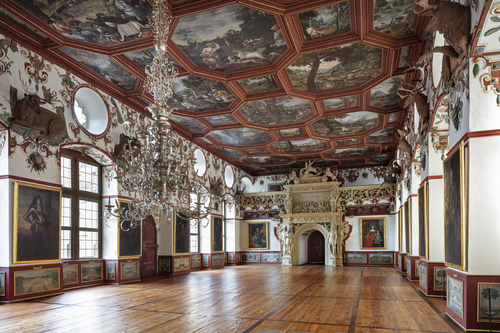
\includegraphics{paintings_files/figure-pdf/cell-3-output-2.png}

Wikibase link:
\url{https://computational-publishing-service.wikibase.cloud/entity/Q213}

Title: Löwenpaar -- Gesamtansicht

Year: 2018

Description: Gerhardt Schmidt, Bildhauer - Mitarbeit: Christoph
Limmerich, Bildhauer - Mitarbeit: Caspar Dieterich, Fassmaler -
Weikersheim, Schloss Weikersheim, Rittersaal \& Raum 72 - Vollendung:
1605 - 1747

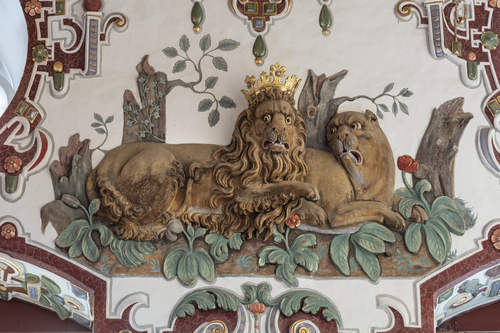
\includegraphics{paintings_files/figure-pdf/cell-3-output-4.png}

Wikibase link:
\url{https://computational-publishing-service.wikibase.cloud/entity/Q214}

Title: Bär -- Gesamtansicht

Year: 2018

Description: Gerhardt Schmidt, Bildhauer - Mitarbeit: Christoph
Limmerich, Bildhauer - Mitarbeit: Caspar Dieterich, Fassmaler -
Weikersheim, Schloss Weikersheim, Rittersaal \& Raum 72 - Vollendung:
1605 - 1747

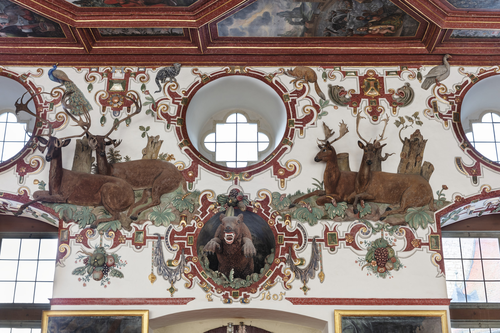
\includegraphics{paintings_files/figure-pdf/cell-3-output-6.png}

Wikibase link:
\url{https://computational-publishing-service.wikibase.cloud/entity/Q215}

Title: Hirschpaare -- Gesamtansicht

Year: 2018

Description: Gerhardt Schmidt, Bildhauer - Mitarbeit: Christoph
Limmerich, Bildhauer - Mitarbeit: Caspar Dieterich, Fassmaler -
Weikersheim, Schloss Weikersheim, Rittersaal \& Raum 72 - Vollendung:
1605 - 1747

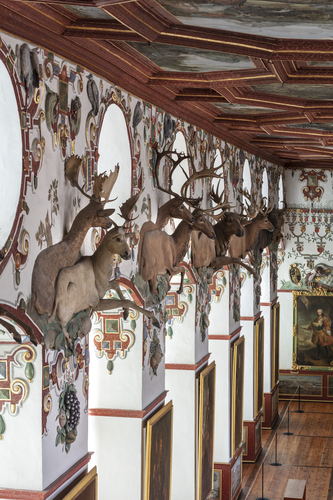
\includegraphics{paintings_files/figure-pdf/cell-3-output-8.png}

Wikibase link:
\url{https://computational-publishing-service.wikibase.cloud/entity/Q216}

Title: Affe -- Gesamtansicht

Year: 2018

Description: Gerhardt Schmidt, Bildhauer - Mitarbeit: Christoph
Limmerich, Bildhauer - Mitarbeit: Caspar Dieterich, Fassmaler -
Weikersheim, Schloss Weikersheim, Rittersaal \& Raum 72 - Vollendung:
1605 - 1747

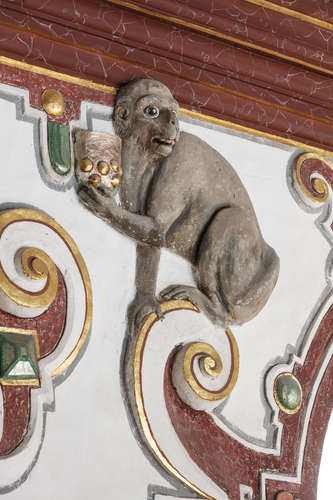
\includegraphics{paintings_files/figure-pdf/cell-3-output-10.png}

Wikibase link:
\url{https://computational-publishing-service.wikibase.cloud/entity/Q220}

Title: Saalbau -- Gartenseite des Schlosses von Süden

Year: 2021

Description: Wolfgang Beringer, Baumeister \& Steinmetz - Georg Stegle,
Baumeister - Entwurf: Georges Robin, Architekt - Elias Gunzenhäuser,
Zimmermann - Weikersheim, Marktplatz 11 - ab 1595

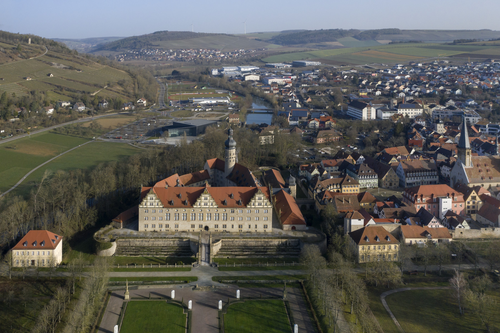
\includegraphics{paintings_files/figure-pdf/cell-3-output-12.png}

Wikibase link:
\url{https://computational-publishing-service.wikibase.cloud/entity/Q221}

Title: Saalbau -- von Südosten

Year: 2021

Description: Wolfgang Beringer, Baumeister \& Steinmetz - Georg Stegle,
Baumeister - Entwurf: Georges Robin, Architekt - Elias Gunzenhäuser,
Zimmermann - Weikersheim, Marktplatz 11 - ab 1595

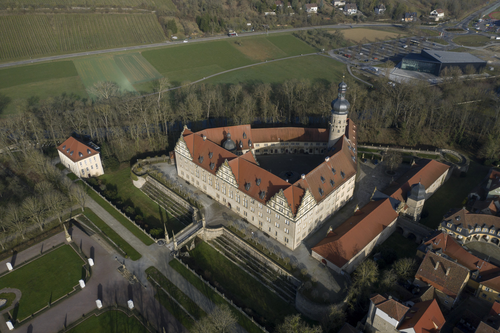
\includegraphics{paintings_files/figure-pdf/cell-3-output-14.png}

Wikibase link:
\url{https://computational-publishing-service.wikibase.cloud/entity/Q224}

Title: Erschließungsraumfolgen

Year: 2020

Description: text

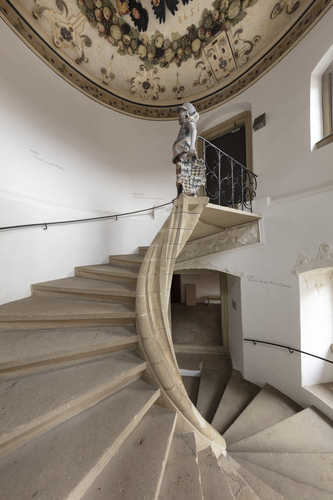
\includegraphics{paintings_files/figure-pdf/cell-3-output-16.png}

Wikibase link:
\url{https://computational-publishing-service.wikibase.cloud/entity/Q225}

Title: Deckendekoration des Treppenturms

Year: 2020

Description: Deckendekoration

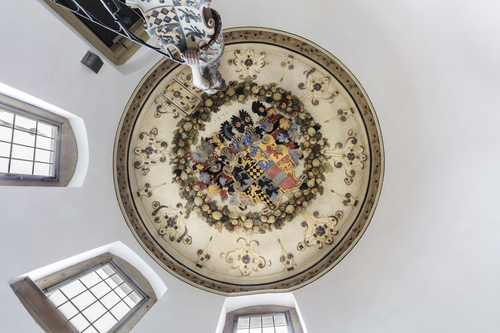
\includegraphics{paintings_files/figure-pdf/cell-3-output-18.png}

Wikibase link:
\url{https://computational-publishing-service.wikibase.cloud/entity/Q230}

Title: Deckendekoration des Rittersaals -- Östliche Partie der Decke

Year: 2018

Description: Balthasar Kazenberger, Maler, 22.09.1601/22.11.1602 - Jan
van der Straet, Maler - Christian Thalwitzer, Restaurator, 1710/1711

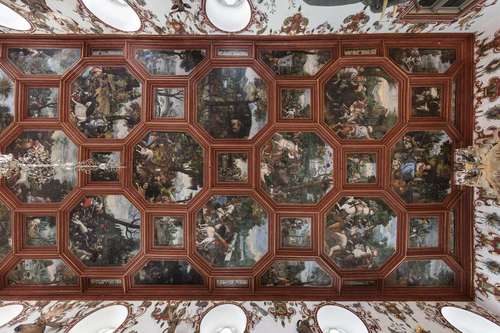
\includegraphics{paintings_files/figure-pdf/cell-3-output-20.png}

Wikibase link:
\url{https://computational-publishing-service.wikibase.cloud/entity/Q234}

Title: Einstige Tafelstube \& Raum 69a -- nach Südosten

Year: 2018

Description: Wolfgang Beringer, Baumeister und Steinmetz - Georg Stegle,
Baumeister - Entwurf: Georges Robin, Architekt - Elias Gunzenhäuser,
Zimmermann - Weikersheim, Marktplatz 11 - ab 1595

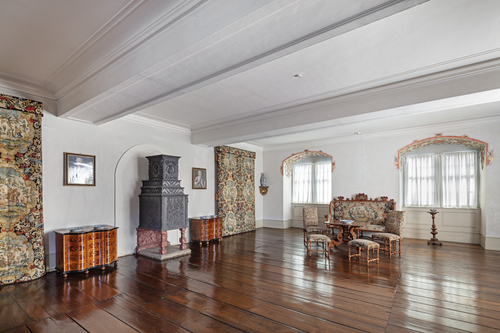
\includegraphics{paintings_files/figure-pdf/cell-3-output-22.png}

Wikibase link:
\url{https://computational-publishing-service.wikibase.cloud/entity/Q251}

Title: Der Saalbau Bild

Year: 2018

Description: Ein Bild vom Saalbau

Bild nicht gefunden

Wikibase link:
\url{https://computational-publishing-service.wikibase.cloud/entity/Q265}

Title: Eroberung der Festung Tottis -- Gesamtansicht

Year: 2018

Description: Teil von: Wanddekoration des Flurs \& Raum 73a
Belagerungsszenen und Türkenschlachten; Balthasar Kazenberger, Maler -
Weikersheim, Schloss Weikersheim, Flur \& Raum 73a - 1603-1604

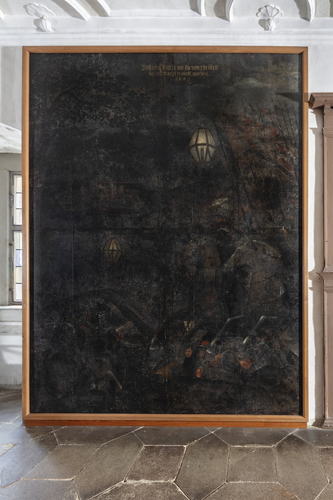
\includegraphics{paintings_files/figure-pdf/cell-3-output-24.png}

Wikibase link:
\url{https://computational-publishing-service.wikibase.cloud/entity/Q267}

Title: Belagerung der Festung Raab -- Gesamtansicht

Year: 2018

Description: Teil von: Wanddekoration des Flurs \& Raum 73a
Belagerungsszenen und Türkenschlachten; Balthasar Kazenberger, Maler -
Weikersheim, Schloss Weikersheim, Flur \& Raum 73a - 1603-1604

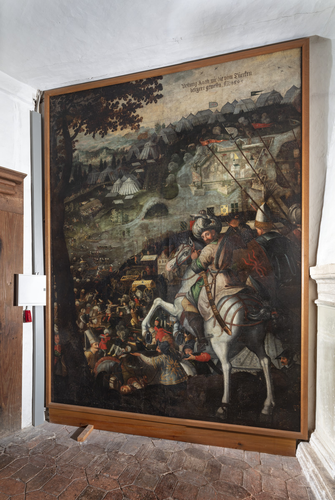
\includegraphics{paintings_files/figure-pdf/cell-3-output-26.png}

Wikibase link:
\url{https://computational-publishing-service.wikibase.cloud/entity/Q268}

Title: Belagerung der Festung Comorna -- Gesamtansicht

Year: 2018

Description: Teil von: Wanddekoration des Flurs \& Raum 73a
Belagerungsszenen und Türkenschlachten; Balthasar Kazenberger, Maler -
Weikersheim, Schloss Weikersheim, Flur \& Raum 73a - 1603-1604

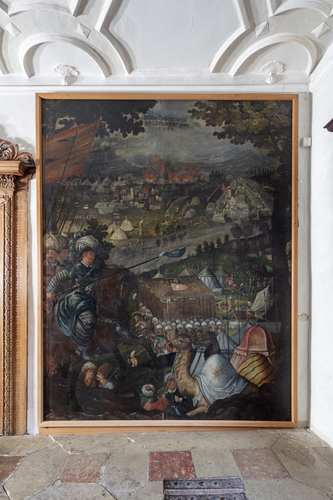
\includegraphics{paintings_files/figure-pdf/cell-3-output-28.png}

Wikibase link:
\url{https://computational-publishing-service.wikibase.cloud/entity/Q269}

Title: Eroberung der Festung Gran -- Gesamtansicht

Year: 2018

Description: Teil von: Wanddekoration des Flurs \& Raum 73a
Belagerungsszenen und Türkenschlachten; Balthasar Kazenberger, Maler -
Weikersheim, Schloss Weikersheim, Flur \& Raum 73a - 1603-1604

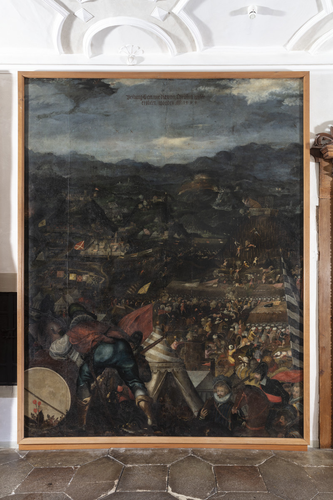
\includegraphics{paintings_files/figure-pdf/cell-3-output-30.png}

Wikibase link:
\url{https://computational-publishing-service.wikibase.cloud/entity/Q270}

Title: Belagerung der Festung von Visegrád -- Gesamtansicht

Year: 2018

Description: Teil von: Wanddekoration des Flurs \& Raum 73a
Belagerungsszenen und Türkenschlachten; Balthasar Kazenberger, Maler -
Weikersheim, Schloss Weikersheim, Flur \& Raum 73a - 1603-1604

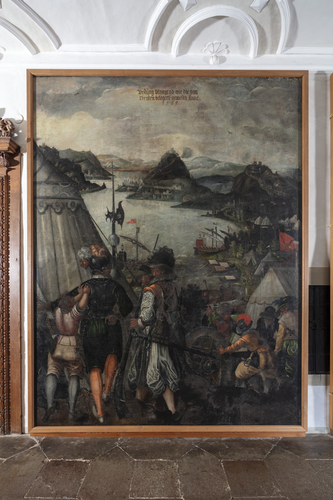
\includegraphics{paintings_files/figure-pdf/cell-3-output-32.png}

Wikibase link:
\url{https://computational-publishing-service.wikibase.cloud/entity/Q271}

Title: Belagerung der Stadt Waitzen -- Gesamtansicht

Year: 2018

Description: Teil von: Wanddekoration des Flurs \& Raum 73a
Belagerungsszenen und Türkenschlachten; Balthasar Kazenberger, Maler -
Weikersheim, Schloss Weikersheim, Flur \& Raum 73a - 1603-1604

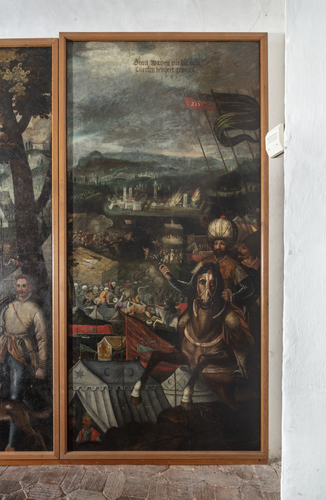
\includegraphics{paintings_files/figure-pdf/cell-3-output-34.png}

Wikibase link:
\url{https://computational-publishing-service.wikibase.cloud/entity/Q272}

Title: Wiedereroberung der Festung Raab -- Gesamtansicht

Year: 2018

Description: Teil von: Wanddekoration des Flurs \& Raum 73a
Belagerungsszenen und Türkenschlachten; Balthasar Kazenberger, Maler -
Weikersheim, Schloss Weikersheim, Flur \& Raum 73a - 1603-1604

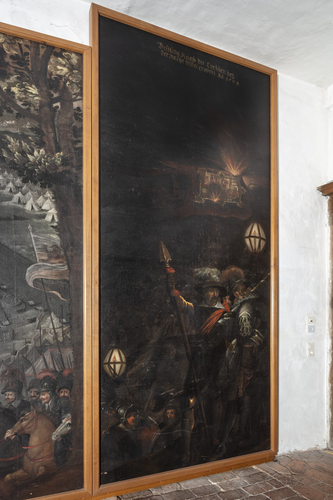
\includegraphics{paintings_files/figure-pdf/cell-3-output-36.png}

Wikibase link:
\url{https://computational-publishing-service.wikibase.cloud/entity/Q273}

Title: Belagerung der Stadt Ofen im Jahr 1598 -- Gesamtansicht

Year: 2018

Description: Teil von: Wanddekoration des Flurs \& Raum 73a
Belagerungsszenen und Türkenschlachten; Balthasar Kazenberger, Maler -
Weikersheim, Schloss Weikersheim, Flur \& Raum 73a - 1603-1604

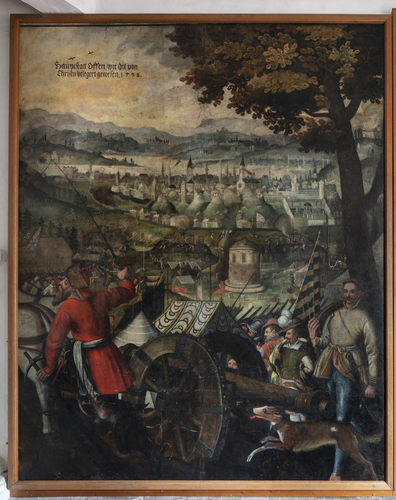
\includegraphics{paintings_files/figure-pdf/cell-3-output-38.png}

Wikibase link:
\url{https://computational-publishing-service.wikibase.cloud/entity/Q274}

Title: Belagerung der Stadt Ofen im Jahr 1603 -- Gesamtansicht

Year: 2018

Description: Teil von: Wanddekoration des Flurs \& Raum 73a
Belagerungsszenen und Türkenschlachten; Balthasar Kazenberger, Maler -
Weikersheim, Schloss Weikersheim, Flur \& Raum 73a - 1603-1604

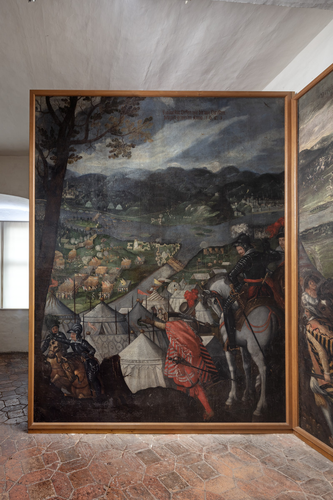
\includegraphics{paintings_files/figure-pdf/cell-3-output-40.png}

Wikibase link:
\url{https://computational-publishing-service.wikibase.cloud/entity/Q275}

Title: Belagerung der Festung Gran -- Gesamtansicht (Anno 1604)

Year: 2018

Description: breites Format; Teil von: Wanddekoration des Flurs \& Raum
73a Belagerungsszenen und Türkenschlachten; Balthasar Kazenberger, Maler
- Weikersheim, Schloss Weikersheim, Flur \& Raum 73a - 1603-1604

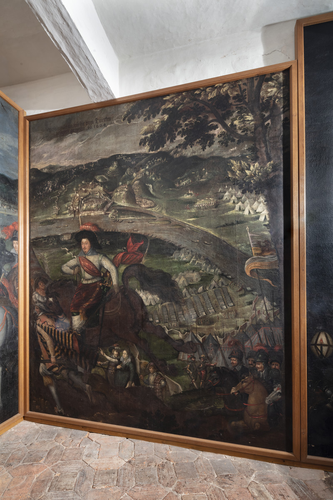
\includegraphics{paintings_files/figure-pdf/cell-3-output-42.png}

Wikibase link:
\url{https://computational-publishing-service.wikibase.cloud/entity/Q276}

Title: Scharmützel bei der Belagerung der Stadt Ofen im Jahr 1603 --
Gesamtansicht

Year: 2018

Description: Teil von: Wanddekoration des Flurs \& Raum 73a
Belagerungsszenen und Türkenschlachten; Balthasar Kazenberger, Maler -
Weikersheim, Schloss Weikersheim, Flur \& Raum 73a - 1603-1604

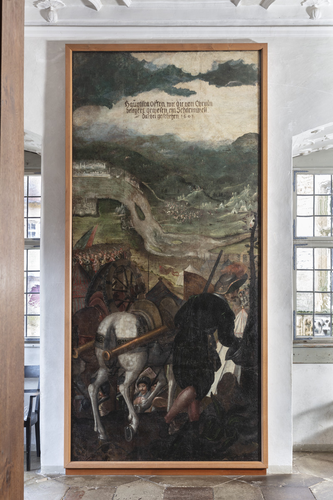
\includegraphics{paintings_files/figure-pdf/cell-3-output-44.png}

Wikibase link:
\url{https://computational-publishing-service.wikibase.cloud/entity/Q266}

Title: Belagerung der Festung Gran -- Gesamtansicht (1594)

Year: 2018

Description: Teil von: Wanddekoration des Flurs \& Raum 73a
Belagerungsszenen und Türkenschlachten; Balthasar Kazenberger, Maler -
Weikersheim, Schloss Weikersheim, Flur \& Raum 73a - 1603-1604

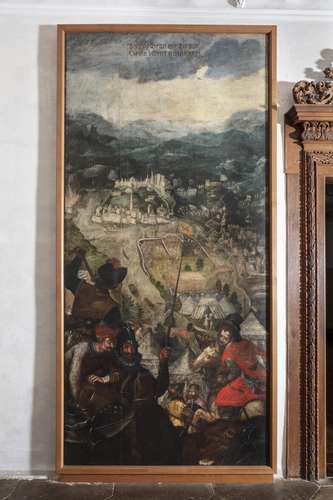
\includegraphics{paintings_files/figure-pdf/cell-3-output-46.png}

Wikibase link:
\url{https://computational-publishing-service.wikibase.cloud/entity/Q283}

Title: Die barocken Schloss- und Gartenveduten bild

Year: 2018

Description: Bild für Die barocken Schloss- und Gartenveduten

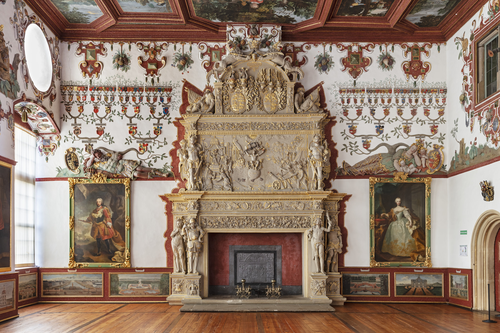
\includegraphics{paintings_files/figure-pdf/cell-3-output-48.png}

Wikibase link:
\url{https://computational-publishing-service.wikibase.cloud/entity/Q288}

Title: Die barocken Schloss- und Gartenveduten bild 2

Year: 2018

Description: Zweites Bild für Die barocken Schloss- und Gartenveduten

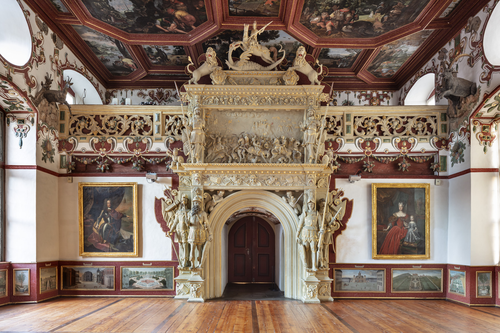
\includegraphics{paintings_files/figure-pdf/cell-3-output-50.png}

Wikibase link:
\url{https://computational-publishing-service.wikibase.cloud/entity/Q289}

Title: Orpheus with the lyre and the animals under a tree

Year: 2021

Description: Balthasar Kazenberger, painter, 22.09.1601/22.11.1602 - Jan
van der Straet, painter- Christian Thalwitzer, restaurator, 1710/1711

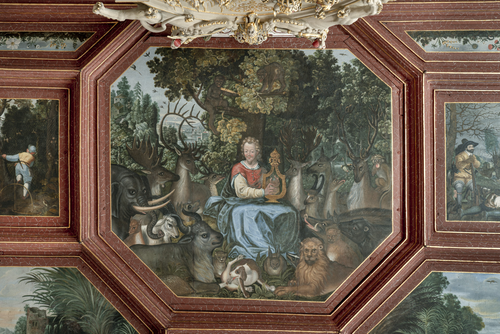
\includegraphics{paintings_files/figure-pdf/cell-3-output-52.png}

Wikibase link:
\url{https://computational-publishing-service.wikibase.cloud/entity/Q292}

Title: Otter catching, with Weikersheim Castle in the background -- on
the left, duck hunting, on the right, otter catching

Year: 2021

Description: Balthasar Kazenberger, painter, 22.09.1601/22.11.1602 - Jan
van der Straet, painter- Christian Thalwitzer, restaurator, 1710/1711

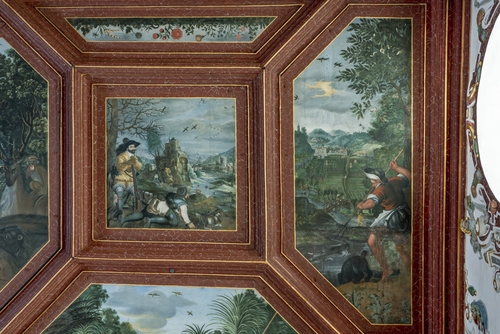
\includegraphics{paintings_files/figure-pdf/cell-3-output-54.png}

Wikibase link:
\url{https://computational-publishing-service.wikibase.cloud/entity/Q200}

Title: Rittersaal \& Raum 72 -- nach Osten

Year: 2018-01-01T00:00:00Z

Description: Teil von: Schloss Weikersheim Saalbau Wolfgang Beringer,
Baumeister \& Steinmetz - Georg Stegle, Baumeister - Entwurf: Georges
Robin, Architekt - Elias Gunzenhäuser, Zimmermann - Weikersheim,
Marktplatz 11 - ab 1595

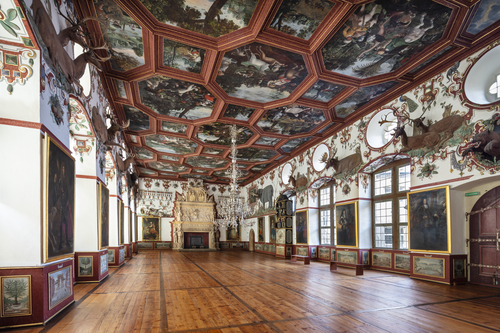
\includegraphics{paintings_files/figure-pdf/cell-3-output-56.png}

Wikibase link:
\url{https://computational-publishing-service.wikibase.cloud/entity/Q211}

Title: Rittersaal \& Raum 72 -- nach Osten

Year: 2018-01-01T00:00:00Z

Description: Teil von: Schloss Weikersheim SaalbauWolfgang Beringer,
Baumeister \& Steinmetz - Georg Stegle, Baumeister - Entwurf: Georges
Robin, Architekt - Elias Gunzenhäuser, Zimmermann - Weikersheim,
Marktplatz 11 - ab 1595

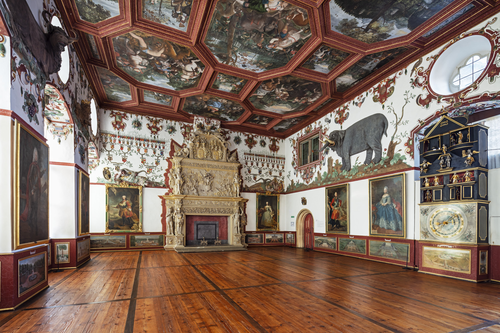
\includegraphics{paintings_files/figure-pdf/cell-3-output-58.png}

Wikibase link:
\url{https://computational-publishing-service.wikibase.cloud/entity/Q212}

Title: Rittersaal \& Raum 72 -- nach Westen

Year: 2018-01-01T00:00:00Z

Description: Teil von: Schloss Weikersheim SaalbauWolfgang Beringer,
Baumeister \& Steinmetz - Georg Stegle, Baumeister - Entwurf: Georges
Robin, Architekt - Elias Gunzenhäuser, Zimmermann - Weikersheim,
Marktplatz 11 - ab 1595

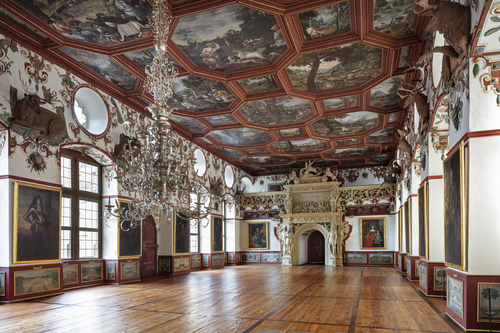
\includegraphics{paintings_files/figure-pdf/cell-3-output-60.png}

Wikibase link:
\url{https://computational-publishing-service.wikibase.cloud/entity/Q213}

Title: Löwenpaar -- Gesamtansicht

Year: 2018-01-01T00:00:00Z

Description: Gerhardt Schmidt, Bildhauer - Mitarbeit: Christoph
Limmerich, Bildhauer - Mitarbeit: Caspar Dieterich, Fassmaler -
Weikersheim, Schloss Weikersheim, Rittersaal \& Raum 72 - Vollendung:
1605 - 1747

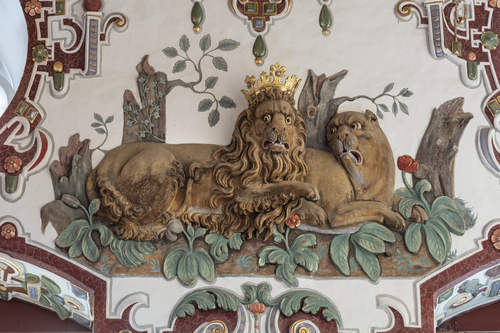
\includegraphics{paintings_files/figure-pdf/cell-3-output-62.png}

Wikibase link:
\url{https://computational-publishing-service.wikibase.cloud/entity/Q214}

Title: Bär -- Gesamtansicht

Year: 2018-01-01T00:00:00Z

Description: Gerhardt Schmidt, Bildhauer - Mitarbeit: Christoph
Limmerich, Bildhauer - Mitarbeit: Caspar Dieterich, Fassmaler -
Weikersheim, Schloss Weikersheim, Rittersaal \& Raum 72 - Vollendung:
1605 - 1747

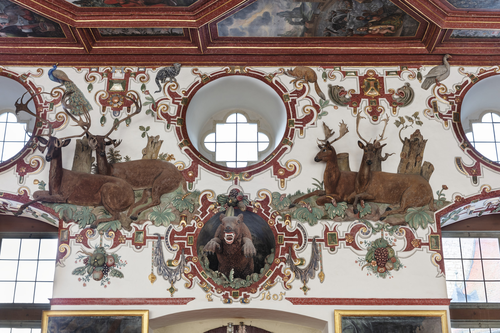
\includegraphics{paintings_files/figure-pdf/cell-3-output-64.png}

Wikibase link:
\url{https://computational-publishing-service.wikibase.cloud/entity/Q215}

Title: Hirschpaare -- Gesamtansicht

Year: 2018-01-01T00:00:00Z

Description: Gerhardt Schmidt, Bildhauer - Mitarbeit: Christoph
Limmerich, Bildhauer - Mitarbeit: Caspar Dieterich, Fassmaler -
Weikersheim, Schloss Weikersheim, Rittersaal \& Raum 72 - Vollendung:
1605 - 1747

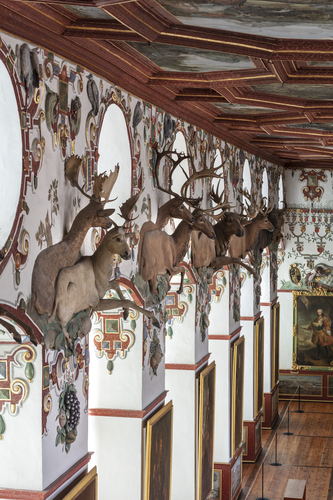
\includegraphics{paintings_files/figure-pdf/cell-3-output-66.png}

Wikibase link:
\url{https://computational-publishing-service.wikibase.cloud/entity/Q216}

Title: Affe -- Gesamtansicht

Year: 2018-01-01T00:00:00Z

Description: Gerhardt Schmidt, Bildhauer - Mitarbeit: Christoph
Limmerich, Bildhauer - Mitarbeit: Caspar Dieterich, Fassmaler -
Weikersheim, Schloss Weikersheim, Rittersaal \& Raum 72 - Vollendung:
1605 - 1747

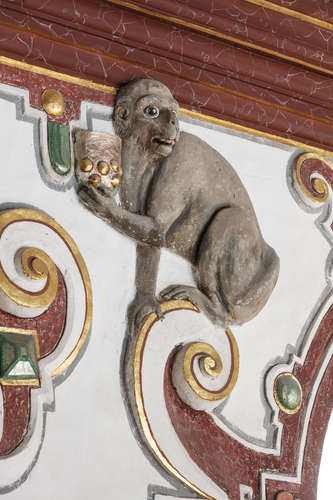
\includegraphics{paintings_files/figure-pdf/cell-3-output-68.png}

Wikibase link:
\url{https://computational-publishing-service.wikibase.cloud/entity/Q230}

Title: Deckendekoration des Rittersaals -- Östliche Partie der Decke

Year: 2018-01-01T00:00:00Z

Description: Balthasar Kazenberger, Maler, 22.09.1601/22.11.1602 - Jan
van der Straet, Maler - Christian Thalwitzer, Restaurator, 1710/1711

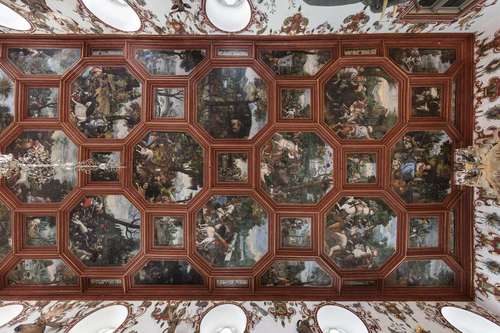
\includegraphics{paintings_files/figure-pdf/cell-3-output-70.png}

Wikibase link:
\url{https://computational-publishing-service.wikibase.cloud/entity/Q224}

Title: Erschließungsraumfolgen

Year: 2020-01-01T00:00:00Z

Description: text

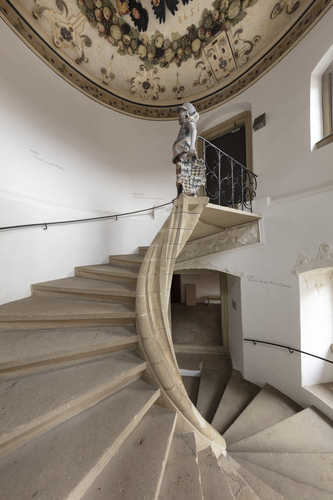
\includegraphics{paintings_files/figure-pdf/cell-3-output-72.png}

Wikibase link:
\url{https://computational-publishing-service.wikibase.cloud/entity/Q220}

Title: Saalbau -- Gartenseite des Schlosses von Süden

Year: 2021-01-01T00:00:00Z

Description: Wolfgang Beringer, Baumeister \& Steinmetz - Georg Stegle,
Baumeister - Entwurf: Georges Robin, Architekt - Elias Gunzenhäuser,
Zimmermann - Weikersheim, Marktplatz 11 - ab 1595

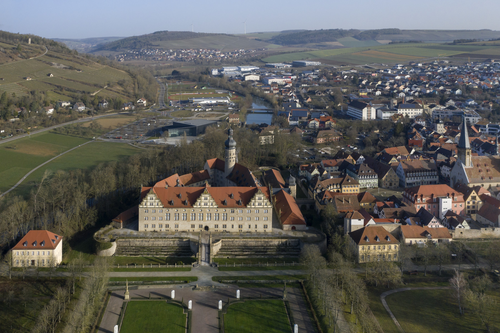
\includegraphics{paintings_files/figure-pdf/cell-3-output-74.png}

Wikibase link:
\url{https://computational-publishing-service.wikibase.cloud/entity/Q221}

Title: Saalbau -- von Südosten

Year: 2021-01-01T00:00:00Z

Description: Wolfgang Beringer, Baumeister \& Steinmetz - Georg Stegle,
Baumeister - Entwurf: Georges Robin, Architekt - Elias Gunzenhäuser,
Zimmermann - Weikersheim, Marktplatz 11 - ab 1595

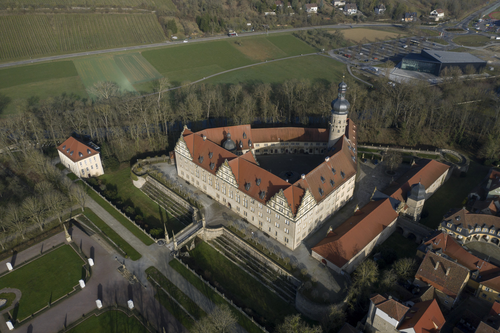
\includegraphics{paintings_files/figure-pdf/cell-3-output-76.png}

Wikibase link:
\url{https://computational-publishing-service.wikibase.cloud/entity/Q234}

Title: Einstige Tafelstube \& Raum 69a -- nach Südosten

Year: 2018-01-01T00:00:00Z

Description: Wolfgang Beringer, Baumeister und Steinmetz - Georg Stegle,
Baumeister - Entwurf: Georges Robin, Architekt - Elias Gunzenhäuser,
Zimmermann - Weikersheim, Marktplatz 11 - ab 1595

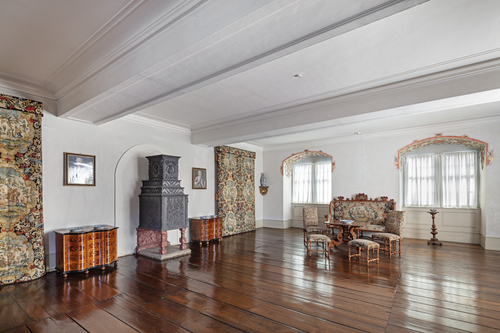
\includegraphics{paintings_files/figure-pdf/cell-3-output-78.png}

Wikibase link:
\url{https://computational-publishing-service.wikibase.cloud/entity/Q225}

Title: Deckendekoration des Treppenturms

Year: 2020-01-01T00:00:00Z

Description: Deckendekoration

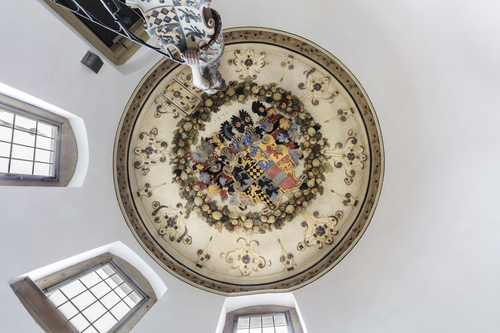
\includegraphics{paintings_files/figure-pdf/cell-3-output-80.png}

Wikibase link:
\url{https://computational-publishing-service.wikibase.cloud/entity/Q251}

Title: Der Saalbau Bild

Year: 2018-01-01T00:00:00Z

Description: Ein Bild vom Saalbau

Bild nicht gefunden

Wikibase link:
\url{https://computational-publishing-service.wikibase.cloud/entity/Q265}

Title: Eroberung der Festung Tottis -- Gesamtansicht

Year: 2018-01-01T00:00:00Z

Description: Teil von: Wanddekoration des Flurs \& Raum 73a
Belagerungsszenen und Türkenschlachten; Balthasar Kazenberger, Maler -
Weikersheim, Schloss Weikersheim, Flur \& Raum 73a - 1603-1604

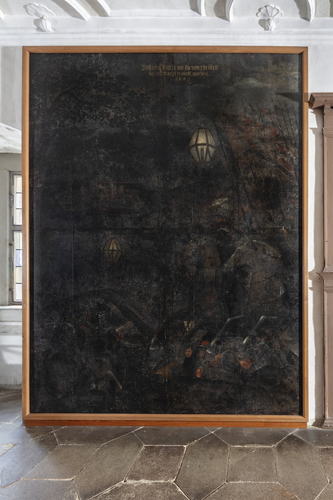
\includegraphics{paintings_files/figure-pdf/cell-3-output-82.png}

Wikibase link:
\url{https://computational-publishing-service.wikibase.cloud/entity/Q267}

Title: Belagerung der Festung Raab -- Gesamtansicht

Year: 2018-01-01T00:00:00Z

Description: Teil von: Wanddekoration des Flurs \& Raum 73a
Belagerungsszenen und Türkenschlachten; Balthasar Kazenberger, Maler -
Weikersheim, Schloss Weikersheim, Flur \& Raum 73a - 1603-1604

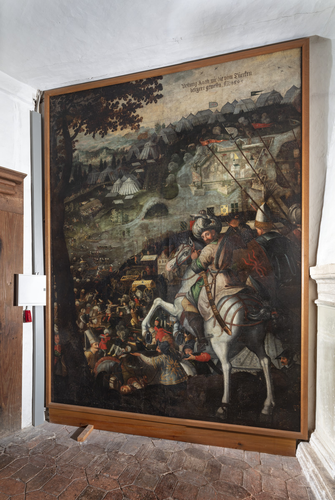
\includegraphics{paintings_files/figure-pdf/cell-3-output-84.png}

Wikibase link:
\url{https://computational-publishing-service.wikibase.cloud/entity/Q268}

Title: Belagerung der Festung Comorna -- Gesamtansicht

Year: 2018-01-01T00:00:00Z

Description: Teil von: Wanddekoration des Flurs \& Raum 73a
Belagerungsszenen und Türkenschlachten; Balthasar Kazenberger, Maler -
Weikersheim, Schloss Weikersheim, Flur \& Raum 73a - 1603-1604

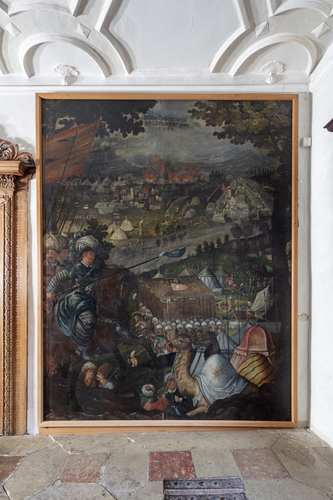
\includegraphics{paintings_files/figure-pdf/cell-3-output-86.png}

Wikibase link:
\url{https://computational-publishing-service.wikibase.cloud/entity/Q269}

Title: Eroberung der Festung Gran -- Gesamtansicht

Year: 2018-01-01T00:00:00Z

Description: Teil von: Wanddekoration des Flurs \& Raum 73a
Belagerungsszenen und Türkenschlachten; Balthasar Kazenberger, Maler -
Weikersheim, Schloss Weikersheim, Flur \& Raum 73a - 1603-1604

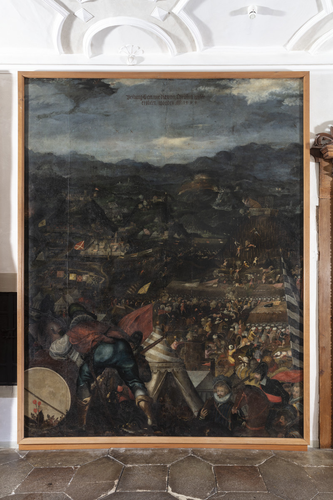
\includegraphics{paintings_files/figure-pdf/cell-3-output-88.png}

Wikibase link:
\url{https://computational-publishing-service.wikibase.cloud/entity/Q270}

Title: Belagerung der Festung von Visegrád -- Gesamtansicht

Year: 2018-01-01T00:00:00Z

Description: Teil von: Wanddekoration des Flurs \& Raum 73a
Belagerungsszenen und Türkenschlachten; Balthasar Kazenberger, Maler -
Weikersheim, Schloss Weikersheim, Flur \& Raum 73a - 1603-1604

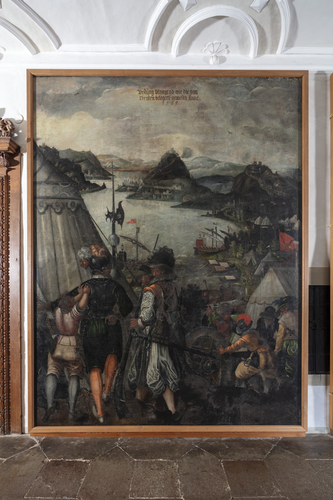
\includegraphics{paintings_files/figure-pdf/cell-3-output-90.png}

Wikibase link:
\url{https://computational-publishing-service.wikibase.cloud/entity/Q271}

Title: Belagerung der Stadt Waitzen -- Gesamtansicht

Year: 2018-01-01T00:00:00Z

Description: Teil von: Wanddekoration des Flurs \& Raum 73a
Belagerungsszenen und Türkenschlachten; Balthasar Kazenberger, Maler -
Weikersheim, Schloss Weikersheim, Flur \& Raum 73a - 1603-1604

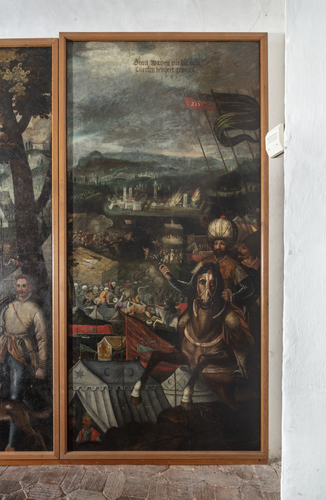
\includegraphics{paintings_files/figure-pdf/cell-3-output-92.png}

Wikibase link:
\url{https://computational-publishing-service.wikibase.cloud/entity/Q272}

Title: Wiedereroberung der Festung Raab -- Gesamtansicht

Year: 2018-01-01T00:00:00Z

Description: Teil von: Wanddekoration des Flurs \& Raum 73a
Belagerungsszenen und Türkenschlachten; Balthasar Kazenberger, Maler -
Weikersheim, Schloss Weikersheim, Flur \& Raum 73a - 1603-1604

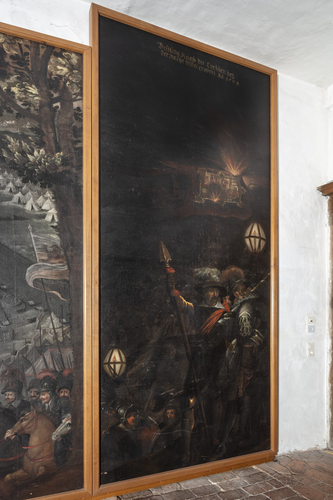
\includegraphics{paintings_files/figure-pdf/cell-3-output-94.png}

Wikibase link:
\url{https://computational-publishing-service.wikibase.cloud/entity/Q273}

Title: Belagerung der Stadt Ofen im Jahr 1598 -- Gesamtansicht

Year: 2018-01-01T00:00:00Z

Description: Teil von: Wanddekoration des Flurs \& Raum 73a
Belagerungsszenen und Türkenschlachten; Balthasar Kazenberger, Maler -
Weikersheim, Schloss Weikersheim, Flur \& Raum 73a - 1603-1604

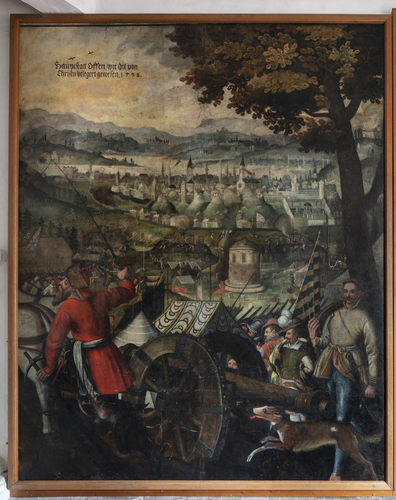
\includegraphics{paintings_files/figure-pdf/cell-3-output-96.png}

Wikibase link:
\url{https://computational-publishing-service.wikibase.cloud/entity/Q274}

Title: Belagerung der Stadt Ofen im Jahr 1603 -- Gesamtansicht

Year: 2018-01-01T00:00:00Z

Description: Teil von: Wanddekoration des Flurs \& Raum 73a
Belagerungsszenen und Türkenschlachten; Balthasar Kazenberger, Maler -
Weikersheim, Schloss Weikersheim, Flur \& Raum 73a - 1603-1604

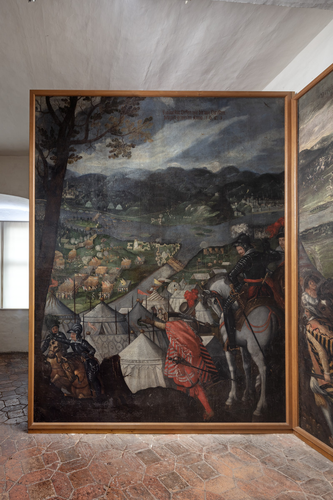
\includegraphics{paintings_files/figure-pdf/cell-3-output-98.png}

Wikibase link:
\url{https://computational-publishing-service.wikibase.cloud/entity/Q275}

Title: Belagerung der Festung Gran -- Gesamtansicht (Anno 1604)

Year: 2018-01-01T00:00:00Z

Description: breites Format; Teil von: Wanddekoration des Flurs \& Raum
73a Belagerungsszenen und Türkenschlachten; Balthasar Kazenberger, Maler
- Weikersheim, Schloss Weikersheim, Flur \& Raum 73a - 1603-1604

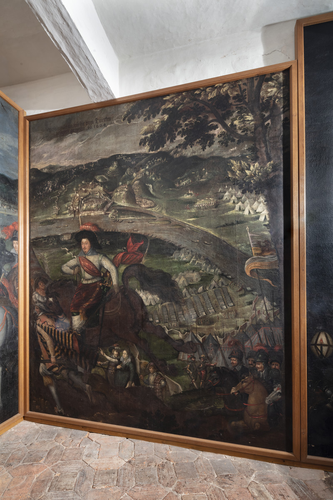
\includegraphics{paintings_files/figure-pdf/cell-3-output-100.png}

Wikibase link:
\url{https://computational-publishing-service.wikibase.cloud/entity/Q276}

Title: Scharmützel bei der Belagerung der Stadt Ofen im Jahr 1603 --
Gesamtansicht

Year: 2018-01-01T00:00:00Z

Description: Teil von: Wanddekoration des Flurs \& Raum 73a
Belagerungsszenen und Türkenschlachten; Balthasar Kazenberger, Maler -
Weikersheim, Schloss Weikersheim, Flur \& Raum 73a - 1603-1604

\includegraphics{paintings_files/figure-pdf/cell-3-output-102.png}

Wikibase link:
\url{https://computational-publishing-service.wikibase.cloud/entity/Q266}

Title: Belagerung der Festung Gran -- Gesamtansicht (1594)

Year: 2018-01-01T00:00:00Z

Description: Teil von: Wanddekoration des Flurs \& Raum 73a
Belagerungsszenen und Türkenschlachten; Balthasar Kazenberger, Maler -
Weikersheim, Schloss Weikersheim, Flur \& Raum 73a - 1603-1604

\includegraphics{paintings_files/figure-pdf/cell-3-output-104.png}

Wikibase link:
\url{https://computational-publishing-service.wikibase.cloud/entity/Q283}

Title: Die barocken Schloss- und Gartenveduten bild

Year: 2018-01-01T00:00:00Z

Description: Bild für Die barocken Schloss- und Gartenveduten

\includegraphics{paintings_files/figure-pdf/cell-3-output-106.png}

Wikibase link:
\url{https://computational-publishing-service.wikibase.cloud/entity/Q288}

Title: Die barocken Schloss- und Gartenveduten bild 2

Year: 2018-01-01T00:00:00Z

Description: Zweites Bild für Die barocken Schloss- und Gartenveduten

\includegraphics{paintings_files/figure-pdf/cell-3-output-108.png}

Wikibase link:
\url{https://computational-publishing-service.wikibase.cloud/entity/Q226}

Title: Schloss

Year: 2020

Bild nicht gefunden

Wikibase link:
\url{https://computational-publishing-service.wikibase.cloud/entity/Q228}

Title: Schloss Weikersheim

Year: 2020

Bild nicht gefunden

Wikibase link:
\url{https://computational-publishing-service.wikibase.cloud/entity/Q289}

Title: Orpheus with the lyre and the animals under a tree

Year: 2021-01-01T00:00:00Z

Description: Balthasar Kazenberger, painter, 22.09.1601/22.11.1602 - Jan
van der Straet, painter- Christian Thalwitzer, restaurator, 1710/1711

\includegraphics{paintings_files/figure-pdf/cell-3-output-110.png}

Wikibase link:
\url{https://computational-publishing-service.wikibase.cloud/entity/Q286}

Title: Wildkatzenjagd - General view

Year: 2021

Bild nicht gefunden

Wikibase link:
\url{https://computational-publishing-service.wikibase.cloud/entity/Q287}

Title: Orpheus with the Lyre and the Animals under a Tree - General View

Year: 2021

Bild nicht gefunden

Wikibase link:
\url{https://computational-publishing-service.wikibase.cloud/entity/Q292}

Title: Otter catching, with Weikersheim Castle in the background -- on
the left, duck hunting, on the right, otter catching

Year: 2021-01-01T00:00:00Z

Description: Balthasar Kazenberger, painter, 22.09.1601/22.11.1602 - Jan
van der Straet, painter- Christian Thalwitzer, restaurator, 1710/1711

\includegraphics{paintings_files/figure-pdf/cell-3-output-112.png}

Wikibase link:
\url{https://computational-publishing-service.wikibase.cloud/entity/Q226}

Title: Schloss

Year: 2020-01-01T00:00:00Z

Bild nicht gefunden

Wikibase link:
\url{https://computational-publishing-service.wikibase.cloud/entity/Q228}

Title: Schloss Weikersheim

Year: 2020-01-01T00:00:00Z

Bild nicht gefunden

Wikibase link:
\url{https://computational-publishing-service.wikibase.cloud/entity/Q286}

Title: Wildkatzenjagd - General view

Year: 2021-01-01T00:00:00Z

Bild nicht gefunden

Wikibase link:
\url{https://computational-publishing-service.wikibase.cloud/entity/Q287}

Title: Orpheus with the Lyre and the Animals under a Tree - General View

Year: 2021-01-01T00:00:00Z

Bild nicht gefunden

Wikibase link:
\url{https://computational-publishing-service.wikibase.cloud/entity/Q200}

Title: Rittersaal \& Raum 72 -- nach Osten

Year: 2018

Description: Teil von: Schloss Weikersheim Saalbau Wolfgang Beringer,
Baumeister \& Steinmetz - Georg Stegle, Baumeister - Entwurf: Georges
Robin, Architekt - Elias Gunzenhäuser, Zimmermann - Weikersheim,
Marktplatz 11 - ab 1595

\includegraphics{paintings_files/figure-pdf/cell-3-output-114.png}

Wikibase link:
\url{https://computational-publishing-service.wikibase.cloud/entity/Q211}

Title: Rittersaal \& Raum 72 -- nach Osten

Year: 2018

Description: Teil von: Schloss Weikersheim SaalbauWolfgang Beringer,
Baumeister \& Steinmetz - Georg Stegle, Baumeister - Entwurf: Georges
Robin, Architekt - Elias Gunzenhäuser, Zimmermann - Weikersheim,
Marktplatz 11 - ab 1595

\includegraphics{paintings_files/figure-pdf/cell-3-output-116.png}

\bookmarksetup{startatroot}

\chapter{Data Visualisation}\label{data-visualisation}

Generate wordcloud

\begin{verbatim}
AttributeError: module 'numpy' has no attribute 'bool8'
---------------------------------------------------------------------------
AttributeError                            Traceback (most recent call last)
Cell In[4], line 1
----> 1 get_graph()

Cell In[3], line 145, in get_graph()
    144 def get_graph():
--> 145     import VizKG.visualize as vkg
    146     results_graph1 = run_query(endpoint_url, query_graph)
    147     #print(results_graph1)
    148     #print('---')

File ~/.local/lib/python3.10/site-packages/VizKG/__init__.py:1
----> 1 from .visualize import *

File ~/.local/lib/python3.10/site-packages/VizKG/visualize.py:3
      1 import sys
      2 import random
----> 3 from .utils import set_chart, set_dataframe, chartdict
      4 from .charts import Chart
      5 class VizKG:

File ~/.local/lib/python3.10/site-packages/VizKG/utils/__init__.py:1
----> 1 from .util import *
      2 from .chartdict import chartdict

File ~/.local/lib/python3.10/site-packages/VizKG/utils/util.py:9
      6 from difflib import SequenceMatcher
      7 import ssl
----> 9 from .chartdict import chartdict as chart_dictionary
     11 def set_chart(chart_input):
     12     """
     13     Setter of chart based on chart input
     14 
   (...)
     17     :return: (str) chart: The available chart   
     18     """

File ~/.local/lib/python3.10/site-packages/VizKG/utils/chartdict.py:1
----> 1 from VizKG.charts import *
      2 """
      3 Dictionary of visualization charts 
      4 """
      5 chartdict = {
      6     'imagegrid': ImageGrid,
      7     'timeline': Timeline,
   (...)
     29     'radarchart': RadarChart
     30 }

File ~/.local/lib/python3.10/site-packages/VizKG/charts/__init__.py:7
      5 from .graph import Graph
      6 from .map import Map
----> 7 from .table import Table
      8 from .imagegrid import ImageGrid
      9 from .dimensions import Dimensions

File ~/.local/lib/python3.10/site-packages/VizKG/charts/table.py:2
      1 from .chart import Chart
----> 2 import plotly.figure_factory as ff
      3 from IPython.display import display
      4 import pandas as pd

File ~/.local/lib/python3.10/site-packages/plotly/figure_factory/__init__.py:32
     30 if optional_imports.get_module("pandas") is not None:
     31     from plotly.figure_factory._county_choropleth import create_choropleth
---> 32     from plotly.figure_factory._hexbin_mapbox import create_hexbin_mapbox
     33 else:
     35     def create_choropleth(*args, **kwargs):

File ~/.local/lib/python3.10/site-packages/plotly/figure_factory/_hexbin_mapbox.py:2
      1 from plotly.express._core import build_dataframe
----> 2 from plotly.express._doc import make_docstring
      3 from plotly.express._chart_types import choropleth_mapbox, scatter_mapbox
      4 import numpy as np

File ~/.local/lib/python3.10/site-packages/plotly/express/__init__.py:15
      9 if pd is None:
     10     raise ImportError(
     11         """\
     12 Plotly express requires pandas to be installed."""
     13     )
---> 15 from ._imshow import imshow
     16 from ._chart_types import (  # noqa: F401
     17     scatter,
     18     scatter_3d,
   (...)
     49     density_mapbox,
     50 )
     53 from ._core import (  # noqa: F401
     54     set_mapbox_access_token,
     55     defaults,
     56     get_trendline_results,
     57     NO_COLOR,
     58 )

File ~/.local/lib/python3.10/site-packages/plotly/express/_imshow.py:4
      2 from _plotly_utils.basevalidators import ColorscaleValidator
      3 from ._core import apply_default_cascade, init_figure, configure_animation_controls
----> 4 from .imshow_utils import rescale_intensity, _integer_ranges, _integer_types
      5 import pandas as pd
      6 import numpy as np

File ~/.local/lib/python3.10/site-packages/plotly/express/imshow_utils.py:24
      9 _integer_types = (
     10     np.byte,
     11     np.ubyte,  # 8 bits
   (...)
     19     np.ulonglong,
     20 )  # 64 bits
     21 _integer_ranges = {t: (np.iinfo(t).min, np.iinfo(t).max) for t in _integer_types}
     22 dtype_range = {
     23     np.bool_: (False, True),
---> 24     np.bool8: (False, True),
     25     np.float16: (-1, 1),
     26     np.float32: (-1, 1),
     27     np.float64: (-1, 1),
     28 }
     29 dtype_range.update(_integer_ranges)
     32 DTYPE_RANGE = dtype_range.copy()

File ~/.local/lib/python3.10/site-packages/numpy/__init__.py:410, in __getattr__(attr)
    407     import numpy.char as char
    408     return char.chararray
--> 410 raise AttributeError("module {!r} has no attribute "
    411                      "{!r}".format(__name__, attr))

AttributeError: module 'numpy' has no attribute 'bool8'
\end{verbatim}

\bookmarksetup{startatroot}

\chapter{Der Große Saal
(Rittersaal)}\label{der-grouxdfe-saal-rittersaal}

\textbf{How to use your own text for processing}

\begin{enumerate}
\def\labelenumi{\arabic{enumi}.}
\tightlist
\item
  Add a new Text item to the wikibase.
  \href{https://computational-publishing-service.wikibase.cloud/wiki/Special:NewItem}{link
  to wikibase new item} the item should contain the following
  statements:
\end{enumerate}

\begin{itemize}
\tightlist
\item
  P57 (external link): link to the html file containing the new text
\item
  P46 (kurator): Item of the curator. you may use an existing item like
  Q210 (Ulrike seeger) for test purposes
\item
  P53 (license): Item of a license for the text. e.g Q203 (CC BY-NC-ND
  4.0 DEED )
\item
  P6 (is part of): set value to Q218 (Schlossanlage Weikersheim)
\end{itemize}

\begin{enumerate}
\def\labelenumi{\arabic{enumi}.}
\setcounter{enumi}{1}
\item
  check if your new text item occurs in the list of selected text items:
  \href{https://computational-publishing-service.wikibase.cloud/query/\#PREFIX\%20cps\%3A\%20\%3Chttps\%3A\%2F\%2Fcomputational-publishing-service.wikibase.cloud\%2Fentity\%2F\%3E\%0APREFIX\%20cpss\%3A\%20\%3Chttps\%3A\%2F\%2Fcomputational-publishing-service.wikibase.cloud\%2Fentity\%2Fstatement\%2F\%3E\%0APREFIX\%20cpsv\%3A\%20\%3Chttps\%3A\%2F\%2Fcomputational-publishing-service.wikibase.cloud\%2Fvalue\%2F\%3E\%0APREFIX\%20cpspt\%3A\%20\%3Chttps\%3A\%2F\%2Fcomputational-publishing-service.wikibase.cloud\%2Fprop\%2Fdirect\%2F\%3E\%0APREFIX\%20cpsp\%3A\%20\%3Chttps\%3A\%2F\%2Fcomputational-publishing-service.wikibase.cloud\%2Fprop\%2F\%3E\%0APREFIX\%20cpsps\%3A\%20\%3Chttps\%3A\%2F\%2Fcomputational-publishing-service.wikibase.cloud\%2Fprop\%2Fstatement\%2F\%3E\%0APREFIX\%20cpspq\%3A\%20\%3Chttps\%3A\%2F\%2Fcomputational-publishing-service.wikibase.cloud\%2Fprop\%2Fqualifier\%2F\%3E\%0A\%0ASELECT\%20\%3FtextItem\%20\%3FkuratorLabel\%20\%3FtextUrl\%0AWHERE\%0A\%7B\%0A\%20\%20\%3FtextItem\%20cpsp\%3AP46\%20\%3FkuratorStatement.\%20\%0A\%20\%20\%3FkuratorStatement\%20cpsps\%3AP46\%20\%3FkuratorItem.\%20\%0A\%20\%20\%3FkuratorItem\%20rdfs\%3Alabel\%20\%3FkuratorLabel.\%0A\%20\%20\%3FtextItem\%20cpsp\%3AP57\%20\%3Furlstatement.\%20\%0A\%20\%20\%3Furlstatement\%20cpsps\%3AP57\%20\%3FtextUrl.\%20\%0A\%7D}{Link
  to wikibase query service}
\item
  set parameter of get\_text() to the id of your new text item e.g.:
  get\_text(``Q209'')
\end{enumerate}

Wikibase link:
\url{https://computational-publishing-service.wikibase.cloud/entity/Q219}

Kurator: Seeger, Ulrike

\bookmarksetup{startatroot}

\chapter{Schlossanlage Weikersheim}\label{schlossanlage-weikersheim-2}

Lorem ipsum dolor sit amet, consectetur adipiscing elit. Integer ut
vehicula purus, vitae viverra ante. Vivamus faucibus sem ac libero
blandit, ut auctor risus porta. Cras non dapibus magna. Curabitur
dignissim est sed porttitor pretium. Fusce ex nunc, dignissim non
bibendum vitae, ultrices non nisl. Sed eget tincidunt enim. Duis
eleifend sapien ac lectus vestibulum rhoncus.

\textbf{How to select images for processing}

Images are selected via the sparql query. The method get\_img() is
capable of using a wikibase item id as parameter to select images with
the property P6 (is part of) linking to the given item id.

\begin{enumerate}
\def\labelenumi{\arabic{enumi}.}
\item
  select a valid location id from the query result:
  \href{https://computational-publishing-service.wikibase.cloud/query/\#PREFIX\%20cps\%3A\%20\%3Chttps\%3A\%2F\%2Fcomputational-publishing-service.wikibase.cloud\%2Fentity\%2F\%3E\%0APREFIX\%20cpss\%3A\%20\%3Chttps\%3A\%2F\%2Fcomputational-publishing-service.wikibase.cloud\%2Fentity\%2Fstatement\%2F\%3E\%0APREFIX\%20cpsv\%3A\%20\%3Chttps\%3A\%2F\%2Fcomputational-publishing-service.wikibase.cloud\%2Fvalue\%2F\%3E\%0APREFIX\%20cpspt\%3A\%20\%3Chttps\%3A\%2F\%2Fcomputational-publishing-service.wikibase.cloud\%2Fprop\%2Fdirect\%2F\%3E\%0APREFIX\%20cpsp\%3A\%20\%3Chttps\%3A\%2F\%2Fcomputational-publishing-service.wikibase.cloud\%2Fprop\%2F\%3E\%0APREFIX\%20cpsps\%3A\%20\%3Chttps\%3A\%2F\%2Fcomputational-publishing-service.wikibase.cloud\%2Fprop\%2Fstatement\%2F\%3E\%0APREFIX\%20cpspq\%3A\%20\%3Chttps\%3A\%2F\%2Fcomputational-publishing-service.wikibase.cloud\%2Fprop\%2Fqualifier\%2F\%3E\%0A\%0ASELECT\%20DISTINCT\%20\%3FpartOfItem\%20\%3FpartOfItemLabel\%0AWHERE\%0A\%7B\%0A\%20\%20\%3FimgItem\%20cpsp\%3AP107\%20\%3FurlStatement.\%20\%0A\%20\%20\%3FurlStatement\%20cpsps\%3AP107\%20\%3FimgUrl.\%20\%0A\%20\%20\%3FimgItem\%20cpsp\%3AP60\%20\%3FdateStatement.\%20\%0A\%20\%20\%3FdateStatement\%20cpsps\%3AP60\%20\%3FpublishDate.\%20\%0A\%20\%20\%3FimgItem\%20cpsp\%3AP6\%20\%3FpartOfStatement.\%0A\%20\%20\%3FpartOfStatement\%20cpsps\%3AP6\%20\%3FpartOfItem.\%0A\%20\%20SERVICE\%20wikibase\%3Alabel\%20\%7B\%0A\%20\%20\%20\%20\%20\%20bd\%3AserviceParam\%20wikibase\%3Alanguage\%20\%22de\%2Cen\%22.\%0A\%20\%20\%20\%20\%20\%20\%3FpartOfItem\%20rdfs\%3Alabel\%20\%3FpartOfItemLabel.\%0A\%20\%20\%20\%20\%20\%20\%3FpartOfItem\%20schema\%3Adescription\%20\%3FpartOfItemDescr.\%0A\%20\%20\%20\%20\%7D\%0A\%7D\%20GROUP\%20BY\%20\%3FpartOfItem\%20\%3FpartOfItemLabel}{Link
  to wikibase query service}
\item
  set parameter of get\_img() to the id of your selected location item
  e.g.: get\_img(``Q217'')
\end{enumerate}

Wikibase link:
\url{https://computational-publishing-service.wikibase.cloud/entity/Q212}

Title: Knight's Hall \& Room 72 - to the west

Year: 2018

Description: Part of: Weikersheim Castle Saalbau Wolfgang Beringer,
builder \& Stonemason - Georg Stegle, master builder - design: Georges
Robin, architect - Elias Gunzenhäuser, carpenter - Weikersheim,
Marktplatz 11 - from 1595

\begin{figure}[H]

{\centering \includegraphics{impressum_files/mediabag/fmd10005862a.jpg}

}

\caption{Knight's Hall \& Room 72 - to the west}

\end{figure}%

Wikibase link:
\url{https://computational-publishing-service.wikibase.cloud/entity/Q213}

Title: Lion couple -- general view

Year: 2018

Description: Gerhardt Schmidt, sculptor - collaboration: Christoph
Limmerich, sculptor - collaboration: Caspar Dieterich, barrel painter -
Weikersheim, Weikersheim Castle, Knight's Hall \& Room 72 - Completion:
1605 - 1747

\begin{figure}[H]

{\centering \includegraphics{impressum_files/mediabag/fmd10005864a.jpg}

}

\caption{Lion couple -- general view}

\end{figure}%

Wikibase link:
\url{https://computational-publishing-service.wikibase.cloud/entity/Q214}

Title: Bear -- general view

Year: 2018

Description: Gerhardt Schmidt, sculptor - collaboration: Christoph
Limmerich, sculptor - collaboration: Caspar Dieterich, barrel painter -
Weikersheim, Weikersheim Castle, Knight's Hall \& Room 72 - Completion:
1605 - 1747

\begin{figure}[H]

{\centering \includegraphics{impressum_files/mediabag/fmd10005865a.jpg}

}

\caption{Bear -- general view}

\end{figure}%

Wikibase link:
\url{https://computational-publishing-service.wikibase.cloud/entity/Q216}

Title: Monkey -- general view

Year: 2018

Description: Gerhardt Schmidt, sculptor - collaboration: Christoph
Limmerich, sculptor - collaboration: Caspar Dieterich, barrel painter -
Weikersheim, Weikersheim Castle, Knight's Hall \& Room 72 - Completion:
1605 - 1747

\begin{figure}[H]

{\centering \includegraphics{impressum_files/mediabag/fmd10005867a.jpg}

}

\caption{Monkey -- general view}

\end{figure}%

Wikibase link:
\url{https://computational-publishing-service.wikibase.cloud/entity/Q215}

Title: Deer pairs -- general view

Year: 2018

Description: Gerhardt Schmidt, sculptor - collaboration: Christoph
Limmerich, sculptor - collaboration: Caspar Dieterich, barrel painter -
Weikersheim, Weikersheim Castle, Knight's Hall \& Room 72 - Completion:
1605 - 1747

\begin{figure}[H]

{\centering \includegraphics{impressum_files/mediabag/fmd10005866a.jpg}

}

\caption{Deer pairs -- general view}

\end{figure}%

Wikibase link:
\url{https://computational-publishing-service.wikibase.cloud/entity/Q200}

Title: Knight's Hall \& Room 72 - to the east

Year: 2018

Description: Part of: Weikersheim Castle SaalbauWolfgang Beringer,
builder \& Stonemason - Georg Stegle, master builder - design: Georges
Robin, architect - Elias Gunzenhäuser, carpenter - Weikersheim,
Marktplatz 11 - from 1595

\begin{figure}[H]

{\centering \includegraphics{impressum_files/mediabag/fmd10005859a.jpg}

}

\caption{Knight's Hall \& Room 72 - to the east}

\end{figure}%

Wikibase link:
\url{https://computational-publishing-service.wikibase.cloud/entity/Q211}

Title: Knight's Hall \& Room 72 - to the east

Year: 2018

Description: Part of: Weikersheim Castle Saalbau Wolfgang Beringer,
builder \& Stonemason - Georg Stegle, master builder - design: Georges
Robin, architect - Elias Gunzenhäuser, carpenter - Weikersheim,
Marktplatz 11 - from 1595

\begin{figure}[H]

{\centering \includegraphics{impressum_files/mediabag/fmd10005860a.jpg}

}

\caption{Knight's Hall \& Room 72 - to the east}

\end{figure}%

\begin{verbatim}
AttributeError: module 'numpy' has no attribute 'bool8'
---------------------------------------------------------------------------
AttributeError                            Traceback (most recent call last)
Cell In[5], line 1
----> 1 get_graph()

Cell In[2], line 142, in get_graph()
    141 def get_graph():
--> 142     import VizKG.visualize as vkg
    143     results_graph1 = run_query(endpoint_url, query_graph)
    144     #print(results_graph1)
    145     #print('---')

File ~/.local/lib/python3.10/site-packages/VizKG/__init__.py:1
----> 1 from .visualize import *

File ~/.local/lib/python3.10/site-packages/VizKG/visualize.py:3
      1 import sys
      2 import random
----> 3 from .utils import set_chart, set_dataframe, chartdict
      4 from .charts import Chart
      5 class VizKG:

File ~/.local/lib/python3.10/site-packages/VizKG/utils/__init__.py:1
----> 1 from .util import *
      2 from .chartdict import chartdict

File ~/.local/lib/python3.10/site-packages/VizKG/utils/util.py:9
      6 from difflib import SequenceMatcher
      7 import ssl
----> 9 from .chartdict import chartdict as chart_dictionary
     11 def set_chart(chart_input):
     12     """
     13     Setter of chart based on chart input
     14 
   (...)
     17     :return: (str) chart: The available chart   
     18     """

File ~/.local/lib/python3.10/site-packages/VizKG/utils/chartdict.py:1
----> 1 from VizKG.charts import *
      2 """
      3 Dictionary of visualization charts 
      4 """
      5 chartdict = {
      6     'imagegrid': ImageGrid,
      7     'timeline': Timeline,
   (...)
     29     'radarchart': RadarChart
     30 }

File ~/.local/lib/python3.10/site-packages/VizKG/charts/__init__.py:7
      5 from .graph import Graph
      6 from .map import Map
----> 7 from .table import Table
      8 from .imagegrid import ImageGrid
      9 from .dimensions import Dimensions

File ~/.local/lib/python3.10/site-packages/VizKG/charts/table.py:2
      1 from .chart import Chart
----> 2 import plotly.figure_factory as ff
      3 from IPython.display import display
      4 import pandas as pd

File ~/.local/lib/python3.10/site-packages/plotly/figure_factory/__init__.py:32
     30 if optional_imports.get_module("pandas") is not None:
     31     from plotly.figure_factory._county_choropleth import create_choropleth
---> 32     from plotly.figure_factory._hexbin_mapbox import create_hexbin_mapbox
     33 else:
     35     def create_choropleth(*args, **kwargs):

File ~/.local/lib/python3.10/site-packages/plotly/figure_factory/_hexbin_mapbox.py:1
----> 1 from plotly.express._core import build_dataframe
      2 from plotly.express._doc import make_docstring
      3 from plotly.express._chart_types import choropleth_mapbox, scatter_mapbox

File ~/.local/lib/python3.10/site-packages/plotly/express/__init__.py:15
      9 if pd is None:
     10     raise ImportError(
     11         """\
     12 Plotly express requires pandas to be installed."""
     13     )
---> 15 from ._imshow import imshow
     16 from ._chart_types import (  # noqa: F401
     17     scatter,
     18     scatter_3d,
   (...)
     49     density_mapbox,
     50 )
     53 from ._core import (  # noqa: F401
     54     set_mapbox_access_token,
     55     defaults,
     56     get_trendline_results,
     57     NO_COLOR,
     58 )

File ~/.local/lib/python3.10/site-packages/plotly/express/_imshow.py:4
      2 from _plotly_utils.basevalidators import ColorscaleValidator
      3 from ._core import apply_default_cascade, init_figure, configure_animation_controls
----> 4 from .imshow_utils import rescale_intensity, _integer_ranges, _integer_types
      5 import pandas as pd
      6 import numpy as np

File ~/.local/lib/python3.10/site-packages/plotly/express/imshow_utils.py:24
      9 _integer_types = (
     10     np.byte,
     11     np.ubyte,  # 8 bits
   (...)
     19     np.ulonglong,
     20 )  # 64 bits
     21 _integer_ranges = {t: (np.iinfo(t).min, np.iinfo(t).max) for t in _integer_types}
     22 dtype_range = {
     23     np.bool_: (False, True),
---> 24     np.bool8: (False, True),
     25     np.float16: (-1, 1),
     26     np.float32: (-1, 1),
     27     np.float64: (-1, 1),
     28 }
     29 dtype_range.update(_integer_ranges)
     32 DTYPE_RANGE = dtype_range.copy()

File ~/.local/lib/python3.10/site-packages/numpy/__init__.py:410, in __getattr__(attr)
    407     import numpy.char as char
    408     return char.chararray
--> 410 raise AttributeError("module {!r} has no attribute "
    411                      "{!r}".format(__name__, attr))

AttributeError: module 'numpy' has no attribute 'bool8'
\end{verbatim}

\bookmarksetup{startatroot}

\chapter{Gemälde-Sammlung: Wikidata
benchmark}\label{gemuxe4lde-sammlung-wikidata-benchmark}

Objective: Make a selection of nine paintings for the exhibition
catalogue to be selected from Wikidata and rendered multi-format in
Quarto.

The below Python code uses SPARQLWrapper to retrieve data from Wikidata
based on a SPARQL query.

This page acts as a `benchmark' to test if data fields can be read from
Wikidata.

Wikidata link: \url{http://www.wikidata.org/entity/Q29474645}

Title: Q29474645

Year: 1789

Creator: Francesco Guardi

Copyright: public domain

\includegraphics{painting-collection_files/figure-pdf/cell-2-output-2.png}

Wikidata link: \url{http://www.wikidata.org/entity/Q29474649}

Title: A Cynical Philosopher

Year: 1650

Creator: Luca Giordano

Copyright: public domain

\includegraphics{painting-collection_files/figure-pdf/cell-2-output-4.png}

Wikidata link: \url{http://www.wikidata.org/entity/Q29474651}

Title: Solomon and the Queen of Sheba

Year: 1697

Creator: Luca Giordano

Copyright: public domain

\includegraphics{painting-collection_files/figure-pdf/cell-2-output-6.png}


\backmatter


\end{document}
